\item C
\item AD
\item BC
\item AC
\item BD
\item BC
\item AD
\item A
\item A
\item $U _ { A B } = \frac { m v _ { 0 } ^ { 2 } } { q }$
\item $E = \frac { 1 } { 6 q } \left ( N _ { b } - N _ { a } \right )$\\ $E _ { k a } = \frac { r } { 12 } \left ( N _ { b } + 5 N _ { a } \right )$\\ $E _ { k b } = \frac { r } { 12 } \left ( 5 N _ { b } + N _ { a } \right )$
\item C
\item C
\item AC
\item BD
\item B
\item D
\item B
\item B
\item A
\item C
\item BD
\item AB
\item BC
\item \begin {enumerate} \item $ O $、$ P $ \item \lmd {1} \quad $ 50.5 $ \item $ 50.0 $ \end {enumerate}
\item \begin {enumerate} \item [(1)] 大约相等 \item [(5)] $m_{1} g t_{12}$ \quad $m_{2}\left (\frac {d}{\Delta t_{2}}-\frac {d}{\Delta t_{1}}\right )$ \item [(6)] $ 0.221 $ \quad $ 0.212 $ \item [(7)] $ 4 $ \end {enumerate}
\item \begin {enumerate} \item $v_{2}=78 \ m/s $ \item $a=2 \ m/s^{2} , t=39 \ s $ \end {enumerate}
\item \begin {enumerate} \item $E=\frac {m v_{0}^{2}}{2 q R}$ \item $v_{1}=\frac {\sqrt {2} v_{0}}{4}$ \item $ 0 $或 $v_{2}=\frac {\sqrt {3} v_{0}}{2}$ \end {enumerate}
\item 减小、减小、小于
\item \begin {enumerate} \item $ \frac { 2 }{ 3 } p $ \item $ \frac { 2 }{ 3 } $ \end {enumerate}
\item BCE
\item \begin {enumerate} \item $\frac {1}{4} l$ \item $\frac {1}{4} f l$ \end {enumerate}
\item D
\item A
\item B
\item D
\item C
\item AD
\item ABC
\item BC
\item 1.84 \quad 1.96 \quad 滑轮的轴不光滑(或滑轮有质量)
\item \begin {enumerate} \item 如图所示: \begin {center} \includesvg [width=0.53\linewidth ]{picture/svg/GZ-3-tiyou-0627} \end {center} \item $I_{1}\left (R_{g1}+R_{0}\right ) \quad I_{2}-I_{1} \quad 180$ \item $ 11.6 $ \item $ 8.0 $ \end {enumerate}
\item \begin {enumerate} \item $B_{\mathrm {m}}=\frac {m v_{0}}{q h}$ \item 粒子会穿过图中 $P$ 点离开磁场, 运动轨迹如图所示。 \begin {center} \includesvg [width=0.53\linewidth ]{picture/svg/GZ-3-tiyou-0629} \end {center} 设粒子在 $P$ 点的运动方向与 $x$ 轴正方向的夹角为 $\alpha $,易得$\alpha =\frac {\pi }{6}$。 \\ $P$ 点与 $x$ 轴的距离为$y=(2-\sqrt {3}) h$。 \end {enumerate}
\item \begin {enumerate} \item 设此时管的加速度大小为$ a_{1} $,方向向下;球的加速度大小为$ a_{2} $,方向向上;$a_{1}=2 g, \quad a_{2}=3 g$。 \item $H_{max}=\frac {13}{25} H$ \item $L \geq \frac {152}{125} H$ \end {enumerate}
\item B \quad C
\item \begin {enumerate} \item 考虑到$ H \gg h>l $,将$ l^{2} $当作二阶小量略去,解得$l=\frac {\rho g H}{p_{0}+\rho g (H+h)} h$,正式答案为$l=\frac {\rho g H}{p_{0}+\rho g H} h$。 \item 解得$V=\left ( 1+\frac {\rho g h}{p_{0}} \right ) S H$,正式答案为$V=\frac {\rho g S H h}{p_{0}}$ \end {enumerate}
\item $ 6.9 \quad 96.8 $
\item \begin {enumerate} \item 如图,设光线在$ D $点的入射角为$ i $,折射角为$ r $。折射光线射到$ BC $边上的$ E $点。设光线在$ E $点的入射角为$ \theta $,由几何关系,有 $\theta =90^{\circ }-\left (30^{\circ }-r\right )>60^{\circ }$。 \begin {center} \includesvg [width=0.45\linewidth ]{picture/svg/GZ-3-tiyou-0633} \end {center} 根据题给数据得 $\sin \theta >\sin 60^{\circ }>\frac {1}{n}$,即 $\theta $ 大于全反射临界角,因此光线在 $E$ 点发生全反射。 \item $\sin r^{\prime }=\frac {2 \sqrt {2}-\sqrt {3}}{4}$ \end {enumerate}
\item B
\item A
\item D
\item B
\item C
\item AC
\item AD
\item BC
\item $ 0.36 \quad 1.80$ \quad $ B $、$ P $之间的距离
\item \begin {enumerate} \item 如图所示。 \begin {center} \includesvg [width=0.23\linewidth ]{picture/svg/GZ-3-tiyou-0652} \end {center} \par \item $ 1.8 $ \item $ 26.0 $,官方答案为:$ 25.5 $ \item $ R_{1} \quad 1.2 $ \end {enumerate}
\item $f=\left \{\begin {array}{l}\frac {2 B^{2} v}{r} x, 0 \leq x \leq \frac {\sqrt {2}}{2} l_{0} \\ \frac {2 B^{2} v}{r}\left (\sqrt {2} l_{0}-x\right ), \frac {\sqrt {2}}{2} l_{0}<x \leq \sqrt {2} l_{0}\end {array}\right .$
\item \begin {enumerate} \item $t_{1}=2.75 \ s$ \item $v_{min}=\sqrt {2} \ m / s, \quad v_{max}=4 \sqrt {3} \ m / s$ \item $I=0$ \end {enumerate}
\item BCD
\item \begin {enumerate} \item $ h=12.9 \ cm $ \item $ T_{2} =363 \ K $ \end {enumerate}
\item 0.4 \quad 10 \quad 负方向
\item 如图($ a $)所示,设从$ D $点入射的光线经折射后恰好射向$ C $点,光在$ AB $边上的入射角为$ \theta 1 $,折射角为$ \theta 2 $。设从$ AD $范围入射的光折射后在$ AC $边上的入射角为$ \theta ^{\prime \prime } $,如图($ b $)所示。 \begin {figure}[h!] \centering \begin {subfigure}{1\linewidth } \centering \includesvg [width=0.85\linewidth ]{picture/svg/GZ-3-tiyou-0653} \caption {}\label {} \end {subfigure} \\ \begin {subfigure}{1\linewidth } \centering \includesvg [width=0.85\linewidth ]{picture/svg/GZ-3-tiyou-0654} \caption {}\label {} \end {subfigure} \end {figure} 易得:$\frac {A C}{C F}=2$
\item C
\item D
\item B
\item A
\item C
\item ABD
\item CD
\item AD
\item AB
\item \begin {enumerate} \item 如图 \begin {center} \includesvg [width=0.93\linewidth ]{picture/svg/GZ-3-tiyou-0675} \end {center} \item 如图 \begin {center} \includesvg [width=0.93\linewidth ]{picture/svg/GZ-3-tiyou-0676} \end {center} \item 非线性 \item BC \end {enumerate}
\item \begin {enumerate} \item 小钢球 \item ①③④② \item $ 9.6 $($ 9.5 \sim 9.7 $都算对) \item 仍能 \end {enumerate}
\item B
\item $\frac {h c}{\lambda _{2}} \quad \frac {h}{\lambda _{1}}$
\item $v=28 \ m / s$
\item AC
\item 有 \quad 增大
\item $Q=2 \times 10^{5} \ J$
\item AB
\item 大 \quad 1.5
\item $d=\frac {f \lambda \Delta t}{2}$
\item \begin {enumerate} \item $E=0.8 \ V$ \item $F=0.8 \ N$ \item $Q=0.32 \ J$ \end {enumerate}
\item \begin {enumerate} \item $v=2 \omega R$ \item $F=\sqrt {\left (2 m \omega ^{2} R\right )^{2}+(m g)^{2}}$ \item $h=\frac {M+16 m}{2 M g}(\omega R)^{2}$ \end {enumerate}
\item \begin {enumerate} \item $d=\frac {m v}{3 q B_{0}}$ \item $\Delta t=\frac {2 \pi m}{q B_{0}}$ \item 比荷的最小值为 $\frac {2 q}{m}$ \end {enumerate}
\item D
\item B
\item A
\item D
\item A
\item C
\item B
\item C
\item AC
\item BD
\item ACD
\item BC
\item \begin {enumerate} \item $ 0.32 $或$ 0.33 $\quad $ 3.1 $ \item $ 9.4 $ \end {enumerate}
\item \begin {enumerate} \item B \item \begin {enumerate} \item 如图: \begin {center} \includesvg [width=0.93\linewidth ]{picture/svg/GZ-3-tiyou-0759} \end {center} \item $ R_{1} $ \item 如图: \begin {center} \includesvg [width=0.93\linewidth ]{picture/svg/GZ-3-tiyou-1708} \end {center} \end {enumerate} \end {enumerate}
\item $\frac {\Delta m}{m}=\frac {1}{3}$
\item \begin {enumerate} \item $d=4.8 \ m$ \item $L=12 \ m$ \end {enumerate}
\item \begin {enumerate} \item $R=\frac {\sqrt {2 m q U}}{q B}$ \quad $L=\frac {\sqrt {2 m q U}}{q B}-\sqrt {\frac {2 m U}{q B^{2}}-d^{2}}$ \item $x=\frac {m d^{2} E}{4 m U-2 q d^{2} B^{2}}$ \item $y=R-\sqrt {R^{2}-d^{2}}+\frac {d^{2}}{\sqrt {R^{2}-d^{2}}}$ \item $s_{1} $、$ s_{2}$、$ s_{3}$ 分别对应气核 ${ }_{1}^{3} \mathrm {H}$、氦去 ${ }_{2}^{4} \mathrm {He}$、质子 ${ }^{1}_{1} \mathrm {H}$ 的位置 \end {enumerate}
\item \begin {enumerate} \item $v_{P 1}=-\frac {3}{5} v_{0}$ \quad $v_{Q 1}=\frac {2}{5} v_{0}$ \item $h_{1}=\frac {v_{0}^{2}}{25 g}$ \\ $h_{2}=\frac {7}{25} \cdot \frac {v_{0}^{2}}{25 g}$ \\ $h_{3}=\left (\frac {7}{25}\right )^{2} \cdot \frac {v_{0}^{2}}{25 g}$\\ 总结可知,第 $n$ 次碰撞后,物块 $Q$ 上升的高度为:\\ $h_{n}=\left (\frac {7}{25}\right )^{n-1} \cdot \frac {v_{0}^{2}}{25 g} \quad (n=1,2,3 \cdots \cdots )$ \item $s=\frac {(8 \sqrt {7}-13) v_{0}^{2}}{200 g \sin \theta }$ \end {enumerate}
\item D
\item A
\item B
\item C
\item B
\item AC
\item AD
\item BC
\item \begin {enumerate} \item AB \item $ 2 $ \item 方便将木板调整到竖直平面 \end {enumerate}
\item \begin {enumerate} \item $ 5 $ \item $ a $ \item $ 2.9 \quad 0.80 $ \end {enumerate}
\item \begin {enumerate} \item $E=0.08 \ V$ \item $F=0.016 \ N$方向垂直于 $a b$ 向左。 \item $P=0.064 \ W$ \end {enumerate}
\item \begin {enumerate} \item $I=m_{1} \sqrt {5 g l}$ \item $E_{\mathrm {k}}=\frac {5 g l\left (2 m_{1}+m_{2}\right )^{2}}{2 m_{2}}$ \end {enumerate}
\item \begin {enumerate} \item $T_{1}=l\sqrt {\frac {m}{2 q U}}$ \item $x=\frac {U}{E}$ \item $m_{1}=\left (\frac {t_{1}}{t_{0}}\right )^{2} m_{0}$ \end {enumerate}
\item C
\item C
\item A
\item C
\item A
\item B
\item B
\item B
\item A
\item D
\item C
\item B
\item D
\item C
\item \begin {enumerate} \item B \item 如图所示 \begin {center} \begin {tikzpicture}[scale=0.5] \draw [gray!70,very thin,step=0.2] (0,0) grid (8,7); \draw [thick] (0,0) grid (8,7); \draw [->] (0,0) node [below left]{$ O $}--(8.5,0) node[above right=1pt] {$ \frac {1}{M}/(kg^{-1}) $} ; \draw [->] (0,0)--(0,7.5) node[right=1pt] {$ a/(m \cdot s^{-2}) $} ; \par \par \draw (2,0) node[below=2pt] {$ 1 $}; \draw (4,0) node[below=2pt] {$ 2 $}; \draw (6,0) node[below=2pt] {$ 3 $}; \draw (8,0) node[below=2pt] {$ 4 $}; \par \par \foreach \x in {1,...,7} { \draw (0,\x ) node[left=2pt] {$ 0.\x $}; } \par \par \par \fill (8,6.2) circle [radius=2pt]; \fill (6.8965,5.6) circle [radius=2pt]; \fill (6.06,4.8) circle [radius=2pt]; \fill (4,3.2) circle [radius=2pt]; \fill (2.816,2.4) circle [radius=2pt]; \fill (2,1.5) circle [radius=2pt]; \fill (5,4) circle [radius=2pt]; \draw [red,thick] (0,0) -- (8,6.5); \end {tikzpicture} \end {center} \item AD \end {enumerate}
\item \begin {enumerate} \item $E^{\prime }=E $,$ r ^{\prime } =r+R_{\mathrm {A}} $。理由如下:\\ 将电源和电流表视为等效电源,电源电动势是电源本身具有的属性,电流表不具有产生电动 势的本领,所以等效电源的电动势仍然为 $E^{\prime }=E $, 而电流表的内阻和电动势的内阻作为等效电源的内阻,即$ r ^{\prime } =r+R_{\mathrm {A}} $。 \item C \quad A \item \subref {2020:北京16:1b} \end {enumerate}
\item \begin {enumerate} \item $x=v_{0} \sqrt {\frac {2 h}{g}}$ \item $v=\sqrt {v_{0}^{2}+2 g h}$ \item $y=\frac {g}{2 v_{0}^{2}} x^{2}$ \end {enumerate}
\item \begin {enumerate} \item $a \rightarrow b$ \item $ E=10 \ V $ \item $ U=9.6 \ V $ \end {enumerate}
\item \begin {enumerate} \item \begin {enumerate} \item 当电压为$ U_{0} $时$v_{0}=\sqrt {\frac {2 e U_{0}}{m}}$ \item 磁感应强度为$ B_{0} $时$v_{0}=\frac {B_{0} q R}{2 m}$(粒子的运动轨迹在水平面内) \end {enumerate} \item $\frac {e \pi ab p^{2} R}{m I}$ \end {enumerate}
\item \begin {enumerate} \item $t=\frac {170}{7} = \approx 24.3 \ s $\\ $ x = \frac {1955}{7} = \approx 279.3 \ m$ \item 列车电气制动产生的加速度与列车的速度成正比,为过$ P $ 点的 正比例函数,论证过程略。画出的图线如下图所示: \begin {center} \includesvg [width=0.93\linewidth ]{picture/svg/GZ-3-tiyou-0813} \end {center} \item 由于空气阻力造成的加速度和电气制动造成的加速度之和依然与速度成正比关系,易知在$ 3 \ m/s $附近所需的机械制动最强。 \end {enumerate}
\item D
\item A
\item D
\item A
\item D
\item A
\item A
\item B
\item A
\item C
\item B
\item C
\item B
\item D
\item B
\item C
\item A
\item C
\item A
\item D
\item A
\item C
\item D
\item D
\item C
\item C
\item D
\item B
\item C
\item A
\item B
\item C
\item B
\item B
\item B
\item 相同 \quad 为零
\item 不需要 \quad \subref {2020上海36a}
\item 需要 \quad \subref {2020上海37b}
\item \begin {enumerate} \item 向左 \item 变大 \end {enumerate}
\item \begin {enumerate} \item $ 10\ m/s $ \item $E_{k}=E_{p}$ \end {enumerate}
\item A
\item B
\item D
\item D
\item A
\item B
\item B
\item C
\item AC
\item AD
\item BD
\item BC
\item BD
\item $\frac {t}{n} \quad \frac {g t^{2}}{4 n^{2} \pi ^{2}}$
\item $15.40 \quad $ 坚直 $\quad 9.74$
\item \begin {enumerate} \item 分压 \item 如图: \begin {center} \includesvg [width=0.7\linewidth ]{picture/svg/GZ-3-tiyou-1704} \end {center} \item 如图: \begin {center} \includesvg [width=0.7\linewidth ]{picture/svg/GZ-3-tiyou-1705} \end {center} \item $1.83 \times 10^{3}$ \item 如图: \begin {center} \includesvg [width=0.7\linewidth ]{picture/svg/GZ-3-tiyou-1706} \end {center} \end {enumerate}
\item \begin {enumerate} \item $ 0.4 \ m $ \item $ 450 \ K $ \end {enumerate}
\item \begin {enumerate} \item $ 30 \ N $ \item $ 0.2 \ m $ \item $ 1 \ s $ \end {enumerate}
\item \begin {enumerate} \item $B=\frac {2 m v_{0}}{q d}$ \item $t=\frac {(11 \pi +3 \sqrt {3}) d}{3 v_{0}}$ \item \begin {enumerate} \item 若三角形$ ABC $区域磁场方向向里,圆形磁场的磁感应强度$B=\frac {6 m v_{0}}{5 q d}$ \item 若三角形$ ABC $区域磁场方向向外,圆形磁场的磁感应强度$B=\frac {2 m v_{0}}{q d}$ \end {enumerate} \end {enumerate}
\item B
\item B
\item D
\item D
\item C
\item B
\item B
\item C
\item C
\item B
\item B
\item A
\item A
\item CD
\item BD
\item AB
\item \begin {enumerate} \item BC \item $ a $ \item $ 0.40 $ \item 不守恒 \end {enumerate}
\item \begin {enumerate} \item $1750(1700 \sim 1800)$ \item 如图 \begin {center} 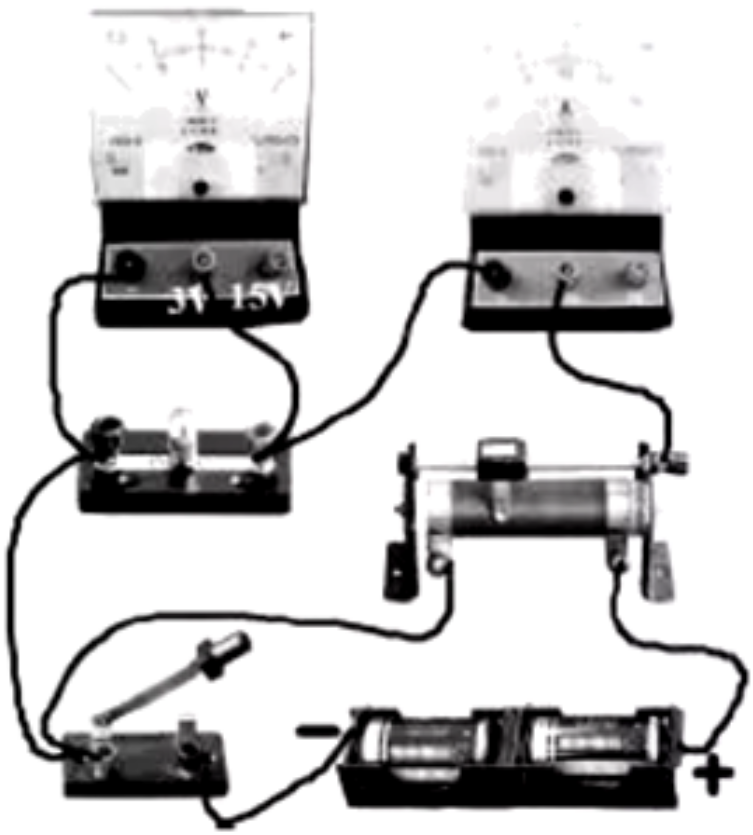
\includegraphics [width=0.7\linewidth ]{picture/screenshot040} \end {center} \begin {center} \includesvg [width=0.7\linewidth ]{picture/svg/GZ-3-tiyou-0697} \end {center} \item C \end {enumerate}
\item \begin {enumerate} \item $v_{m}=18 \ m/s$ \item $t_{1}=6 \ s $ \item $ F_{f}=180 \ N$ \end {enumerate}
\item \begin {enumerate} \item $v_{F}=1 \ m / s$ \item $E_{p 0}=8.0 \times 10^{-3} \ J$ \item $ E_{p}=m g h+\mu m g\left (L_{1}+L_{2}\right ) $\\ $ E_{p}=2 \times 10^{-3}(10 h+3) \ J $ \end {enumerate}
\item \begin {enumerate} \item $-\frac {B l U_{m}}{R} \sin \frac {2 \pi }{T} t$ \item $I_{F}=\frac {B l U_{m} T}{2 \pi R}+\frac {m U_{m}}{B l}$ \item \begin {enumerate} \item 当 $F_{A}=-F$ 时\\ $ x=0, v=\pm v_{in}=\pm 1\ m / s$ \item 当 $F_{A}=F$ 时\\ $x_{1}^{\prime }=\frac {1}{\sqrt {5}} \ m$ 和 $v_{1}^{\prime }=\frac {2}{\sqrt {5}} \ m / s $\\ $ x_{2}^{\prime }=-\frac {1}{\sqrt {5}} \ m$ 和 $v_{2}^{\prime }=-\frac {2}{\sqrt {5}} \ m$ \end {enumerate} \end {enumerate}
\item \begin {enumerate} \item $ ^{1}_{0}n \rightarrow ^{1}_{1}P + ^{0}_{-1}e + ^{0}_{0} \bar {\nu _{e}} $\\ $E_{e}+E_{v}=0.7468 \ MeV$ \item $\eta =\frac {2}{3}$ \item $B=\frac {3}{200 a} \ T \quad (B \geqslant \frac {\sqrt {15}}{40} \ T) $ \end {enumerate}
\item B
\item B
\item A
\item D
\item D
\item C
\item C
\item D
\item C
\item D
\item C
\item B
\item C
\item BC
\item CD
\item BD
\item \begin {enumerate} \item $0.18 \sim 0.19$ \item $ a $ \item $ a $和$ b $ \par \end {enumerate}
\item \begin {enumerate} \item BC \item C \end {enumerate}
\item \begin {enumerate} \item 电路图: \begin {center} \includesvg [width=0.6\linewidth ]{picture/svg/GZ-3-tiyou-0728} \end {center} \item $0.39 \sim 0.41$ \item $1.29 \sim 1.31$ \item $ b $ \item $1.51 \sim 1.54$ \item $0.52 \sim 0.54$ \end {enumerate}
\item \begin {enumerate} \item $ a=0.125\ m/s^{2} $竖直向下; \item $ v=1 \ m/s $; \item $ x=40 \ m $ \end {enumerate}
\item \begin {enumerate} \item $ F_{N}=8 \ N $,方向水平向左; \item 能在斜轨道上到达的最高点为 $C^{\prime }$ 点,由于$L_{BC^{\prime }}=\frac {15}{16} m<1$,不会冲出; \item $ h= \left \{ \begin {aligned} &\frac {1}{6} x-\frac {5}{48} \quad &\left (\frac {5}{8} m<x \leq 1 \ m\right )\\ &0 \quad &\left (0 \leq x \leq \frac {5}{8} \ m\right ) \end {aligned} \right . $ \end {enumerate}
\item \begin {enumerate} \item $ F=0.0625 \ N $ \item $B=\frac {1}{6-4 t}$ \item $ q=0.5 \ C $ \end {enumerate}
\item \begin {enumerate} \item $v=\frac {q B R}{m}, \quad s=0.8 R$ \item $L_{\max }=\frac {4}{15} R$ \item $ F= \left \{ \begin {aligned} &2.6 NqBR &0<L \leq \frac {4}{15} R\\ &1.8 NqBR &\frac {4}{15} R<L \leq 0.4 R\\ &N q B R &L>0.4 R \end {aligned} \right . $ \end {enumerate}
\item A
\item D
\item B
\item \par 
\item B
\item \par 
\item C
\item \par 
\item BD
\item \par 
\item BC
\item \par 
\item AC
\item A
\item $ 0.233 $
\item $ 0.75 $
\item \begin {enumerate} \item C \item AC \item $\frac {99}{79}$ \end {enumerate}
\item \begin {enumerate} \renewcommand {\labelenumi }{\arabic {enumi}.} \item $\frac {q}{m}=\frac {4 U}{B^{2} d^{2}}$ \item $t=\frac {B d^{2}}{4 U}\left (\frac {\pi }{2}+\frac {\sqrt {3}}{3}\right )$ \par \end {enumerate} \par \par 
\item \begin {enumerate} \renewcommand {\labelenumi }{\arabic {enumi}.} \item $m^{\prime }=3 m$ \item $W=\frac {2}{15} m g H$ \item $\frac {\mu }{\mu ^{\prime }}=\frac {11}{9}$ \end {enumerate} \par \par 
\item 低于
\item 大于
\item \begin {enumerate} \renewcommand {\labelenumi }{\arabic {enumi}.} \item $p_{2}=3.2 \times 10^{7} \ \mathrm {Pa}$ \item $p_{3}=1.6 \times 10^{8} \mathrm {Pa}$ \par \end {enumerate} \par \par 
\item CDE
\item \begin {enumerate} \renewcommand {\labelenumi }{\arabic {enumi}.} \item $x=7 \ \mathrm {m}$ \par \item $=x^{\prime }=(6 \sqrt {2}-3) \ m \approx 5.5 \ m$ \end {enumerate} \par \par 
\item B
\item A
\item D
\item \par 
\item B
\item \par 
\item C
\item \par 
\item AD
\item \par 
\item BC
\item \par 
\item AB
\item \par 
\item $ 3.775 $
\item $ 53.7 $
\item $ b $
\item $ 450 $
\item $ 620.0 $
\item $ 33.0 $
\item \par 
\item \begin {enumerate} \renewcommand {\labelenumi }{\arabic {enumi}.} \item $t=\frac {1}{g} \sqrt {\frac {2 E}{m}}$ \item $h=h_{1}+h_{2}=\frac {2 E}{m g}$ \par \end {enumerate} \par \par 
\item \begin {enumerate} \renewcommand {\labelenumi }{\arabic {enumi}.} \item $s_{1}=\frac {2 \sqrt {3}}{3} h$ \item $B=\sqrt {\frac {6 m E}{q h}}$ \item $s_{2}^{\prime }-s_{2}=\frac {2 \sqrt {3}}{3}(\sqrt {2}-1) h$ \end {enumerate} \par \par 
\item BDE
\item $m=\frac {15 p_{0} S}{26 g}$
\item $\sqrt {3}$
\item 大于
\item \begin {enumerate} \renewcommand {\labelenumi }{\arabic {enumi}.} \item 波沿负方向传播 \item $x_{Q}=9\ \mathrm {cm}$ \par \end {enumerate} \par \par 
\item A
\item C
\item B
\item B
\item A
\item BC
\item AC
\item \par 
\item AD
\item \par 
\item 从右向左
\item $ 0.19 $
\item $ 0.037 $
\item 实验电路原理图如图所示 \includesvg [width=0.23\linewidth ]{picture/svg/GZ-3-tiyou-0585}
\item 增大
\item 增大
\item $ 0.39 $
\item $ 1.17 $
\item \par 
\item \begin {enumerate} \renewcommand {\labelenumi }{\arabic {enumi}.} \item $E_{k 0}=4.0 \times 10^{8} \mathrm {J}$ \quad $E_{h}=2.4 \times 10^{12} \ \mathrm {J}$ \item $W=9.7 \times 10^{8} \ \mathrm {J}$ \par \end {enumerate} \par \par 
\item \begin {enumerate} \renewcommand {\labelenumi }{\arabic {enumi}.} \item $v_{2}=v_{0}-2 g t_{1}$ \item 若$ B $点在$ A $点之上,$E_{2}=\left [2-2 \frac {v_{0}}{g t_{1}}+\frac {1}{4}\left (\frac {v_{0}}{g t_{1}}\right )^{2}\right ] E_{1}$ \quad 为使 $E_{2}>E_{1},$ 应有$2-2 \frac {v_{0}}{g t_{1}}+\frac {1}{4}\left (\frac {v_{0}}{g t_{1}}\right )^{2}>1$。即当 $0<t_{1}<\left (1-\frac {\sqrt {3}}{2}\right ) \frac {v_{0}}{g}$或 $t_{1}>\left (1+\frac {\sqrt {3}}{2}\right ) \frac {v_{0}}{g}$才是可能的; \\ 若 $B$ 在 $A$ 点之下,$E_{2}=\left [2-2 \frac {v_{0}}{g t_{1}}-\frac {1}{4}\left (\frac {v_{0}}{g t_{1}}\right )^{2}\right ] E_{1}$。为使 $E_{2}>E_{1},$ 应有 $2-2 \frac {v_{0}}{g t_{1}}-\frac {1}{4}\left (\frac {v_{0}}{g t_{1}}\right )^{2}>1$ 即 $t_{1}>\left (\frac {\sqrt {5}}{2}+1\right ) \frac {v_{0}}{g}$ 另一解为负,不符合题意 \par \par \end {enumerate} \par \par 
\item ABC
\item \begin {enumerate} \renewcommand {\labelenumi }{\arabic {enumi}.} \item $p_{1}=2 p_{0}$ \item $p_{2}^{\prime }=\frac {3}{2} p_{0}$ \item $p_{3}=1.6 p_{0}$ \par \end {enumerate} \par \par 
\item 2
\item 减弱
\item 加强
\item $n=\sqrt {2.05} \approx 1.43$
\item D
\item A
\item 0.8
\item $ 10 \ s $和$ 14 \ s $
\item BC
\item A
\item B
\item D
\item D
\item B
\item A
\item B
\item B
\item C
\item C
\item B
\item $ 7:9 $
\item 2.1
\item A
\item $a = 5\ \mathrm { m } / \mathrm { s } ^ { 2 }$, 设加速阶段通过的距离为$ S ^{\prime } =10\ m $
\item \begin {enumerate} \renewcommand {\labelenumi }{\arabic {enumi}.} \item $v = 37.5 \ \mathrm { m } / \mathrm { s }$ \item $ a=1.35\ m/s^{2} $ \par \end {enumerate} \par \par 
\item C
\item $ 20\ m/s $
\item $\frac { s } { s ^ { \prime } } = \frac { 5 } { 7 }$
\item \begin {enumerate} \renewcommand {\labelenumi }{\arabic {enumi}.} \item $ s=1950\ m $ \item $ M=3\times 10^{-9} \times 6.8 \times 10^{8} \ kg = 2.04\ kg $ \par \end {enumerate} \par \par 
\item \par \begin {enumerate} \renewcommand {\labelenumi }{\arabic {enumi}.} \item $\frac { v _ { 0 } ^ { 2 } - v _ { 1 } ^ { 2 } } { 2 g s _ { 0 } }$ \item $\frac { s _ { 1 } \left ( v _ { 0 } + v _ { 1 } \right ) ^ { 2 } } { 2 s _ { 0 } ^ { 2 } }$ \par \par \par \end {enumerate} \par \par \par 
\item $v = \frac { 1 } { 4 } \sqrt { 6 a l }$
\item C
\item \begin {enumerate} \renewcommand {\labelenumi }{\arabic {enumi}.} \item $ x=16\ m $ \item 上滑过程:$a _ { 1 } = g \sin \theta + \mu g \cos \theta $ 有$ a_1=8\ m/s^{2} $, \\ 下滑过程: $a _ { 2 } = g \sin \theta - \mu g \cos \theta $有$ a_2=4\ m/s^{2} $, \item $v = 2 \sqrt { 34 } \mathrm { m } / \mathrm { s }$ \par \end {enumerate} \par \par 
\item C
\item C
\item A
\item C
\item A
\item B
\item C
\item A
\item A
\item B
\item \begin {enumerate} \renewcommand {\labelenumi }{\arabic {enumi}.} \item $ a=1.5\ m/s^{2} $ \par \item $ \bar {v}=20\ m/s $ \par \end {enumerate} \par \par 
\item A
\item A
\item B
\item D
\item B
\item A
\item D
\item BD
\item BD
\item CD
\item A
\item BD
\item BD
\item \begin {enumerate} \renewcommand {\labelenumi }{\arabic {enumi}.} \item $a _ { 1 } = \frac { \Delta v } { \Delta t } = \frac { 4.2 - 0 } { 40 } = 0.105 \ \mathrm { m } / \mathrm { s } ^ { 2 }$\\ $x _ { 1 } = \frac { 1 } { 2 } v t = \frac { 1 } { 2 } \times 4.2 \times 40 = 84 \mathrm { m }$ \par \item $ F=400\ N $ \item $ 3.86\ m/s $ \par \end {enumerate} \par \par 
\item D
\item D
\item A
\item AD
\item AD
\item C
\item D
\item CD
\item B
\item A
\item B
\item D
\item A
\item BC
\item C
\item C
\item B
\item AD
\item C
\item AC
\item B
\item AC
\item BD
\item AD
\item A
\item BCD
\item A
\item AC
\item A
\item BC
\item B
\item C
\item D
\item C
\item BD
\item B
\item B
\item D
\item A
\item A
\item A
\item C
\item D
\item A
\item BD
\item AD
\item C
\item B
\item A
\item AB
\item A
\item D
\item C
\item BD
\item \par 
\item \par 
\item A
\item A
\item 0.248
\item 等于
\item \begin {enumerate} \renewcommand {\labelenumi }{\arabic {enumi}.} \item $ -3qEl \cos \theta $ \item $ 30 ^{\circ } $ \item 当$ \theta < 150 ^{ \circ } $时,$\omega = \sqrt { \frac { 2 \sqrt { 3 } ( 1 - \sin \theta ) - 6 \cos \theta } { 5 \sqrt { 3 } l } g }$ \par \end {enumerate} \par \par 
\item 运动状态
\item 惯性
\item C
\item C
\item C
\item C
\item A
\item B
\item $ F=9\ N $
\item A
\item D
\item \begin {enumerate} \renewcommand {\labelenumi }{\arabic {enumi}.} \item $ 0.2\ N $ \item $ 0.375\ m $ \par \par \end {enumerate} \par \par 
\item A
\item BC
\item BD
\item CD
\item \begin {enumerate} \renewcommand {\labelenumi }{\arabic {enumi}.} \item $\frac { a v ^ { 2 } } { 2 a s - v ^ { 2 } }$ \item $0 \qquad m ( a \cot \theta - g )$ \par \par \end {enumerate} \par \par 
\item C
\item A
\item \begin {enumerate} \renewcommand {\labelenumi }{\arabic {enumi}.} \item $k = \frac { F _ { 0 } } { x _ { 0 } } = \frac { 8 m g \sin \theta } { 5 x _ { 0 } }$ \item $a = \frac { 1 } { 5 } g \sin \theta $ \item $F = \frac { 8 } { 25 } m g \sin \theta + k x = \frac { 8 } { 25 } m g \sin \theta + \frac { 1 } { 2 } k a t ^ { 2 } = \frac { 4 } { 25 } m g \sin \theta \left ( 2 + \frac { g \sin \theta } { x _ { 0 } } \cdot t ^ { 2 } \right )$ \par \par \end {enumerate} \par \par 
\item 减速上升或加速下降
\item AD
\item C
\item AC
\item B
\item D
\item B
\item BD
\item A
\item D
\item A
\item A
\item A
\item D
\item D
\item D
\item BC
\item B
\item BD
\item BD
\item AB
\item C
\item \begin {enumerate} \renewcommand {\labelenumi }{\arabic {enumi}.} \item $\frac { 50 } { 11 } m$ \item $0 ; - \frac { 10 } { 11 };$ \item $\frac { 10 } { 11 } s , \frac { 10 \sqrt { 11 } } { 33 } s$ \par \end {enumerate} \par \par 
\item \begin {enumerate} \renewcommand {\labelenumi }{\arabic {enumi}.} \item 物块与木板$ \mu _{1}=0.20 $ ,木板与地面$ \mu _{2}=0.30 $ \item $ s=1.125\ m $ \par \par \end {enumerate} \par \par 
\item \begin {enumerate} \renewcommand {\labelenumi }{\arabic {enumi}.} \item $v _ { A } = \sqrt { 2 \mu g L }$ \item $a _ { B } = 3 \mu g , \quad a _ { B } ^ { \prime } = \mu g$ \item $v _ { B } = 2 \sqrt { 2 \mu g L }$ \par \par \end {enumerate} \par \par 
\item \begin {enumerate} \renewcommand {\labelenumi }{\arabic {enumi}.} \item $v _ { A 1 } = \sqrt { 2 g H }$ \item $f _ { A } = m g \left ( \frac { H } { h _ { A } } - \frac { 1 } { 9 } \right )$ \item $f _ { A }: f _ { B } = \frac { \left ( 9 H - h _ { A } \right ) h _ { B } } { \left ( 9 H - h _ { B } \right ) h _ { A } }$ \par \end {enumerate} \par \par 
\item \begin {enumerate} \renewcommand {\labelenumi }{\arabic {enumi}.} \item $k = m g \tan \theta _ { 0 } / v _ { 0 }$ \item $\tan \theta = a / g + v \tan \theta _ { 0 } / v _ { 0 }$ \item $\sin \beta \leq \frac { 2 r \cos \theta _ { 0 } } { g \left ( \frac { s } { v _ { 0 } } - \frac { v _ { 0 } } { 2 a } \right ) ^ { 2 } }$ \par \par \par \end {enumerate} \par \par 
\item \begin {enumerate} \renewcommand {\labelenumi }{\arabic {enumi}.} \item $\mu = \frac { f } { m g } = \frac { 10 } { 2 \times 10 } = 0.5$ \item $t = \sqrt { \frac { 2 s } { a } } = \sqrt { \frac { 2 \times 6.06 } { 11.5 } } = 1.03 ( s )$ \par \end {enumerate} \par \par 
\item \begin {enumerate} \renewcommand {\labelenumi }{\arabic {enumi}.} \item $ a=8\ m/s^{2} $ \item $ \Delta t=0.3\ s $ \item $\frac { F _ { 0 } } { m g } = \frac { \sqrt { 41 } } { 5 }$ \par \end {enumerate} \par \par 
\item \begin {enumerate} \renewcommand {\labelenumi }{\arabic {enumi}.} \item $f = \mu \left ( 2 m _ { 1 } + m _ { 2 } \right ) g$ \item $F > 2 \mu \left ( m _ { 1 } + m _ { 2 } \right ) g$ \item $F = 22.4\ N$ \par \end {enumerate} \par \par 
\item \begin {enumerate} \renewcommand {\labelenumi }{\arabic {enumi}.} \item $ a=3\ m/s^{2} \qquad v=8\ m/s $ \item $F _ { \min } = \frac { 13 \sqrt { 3 } } { 5 } N$ \par \end {enumerate} \par \par 
\item \begin {enumerate} \renewcommand {\labelenumi }{\arabic {enumi}.} \item $ S_{1}=30 \ m $ \item $ \Delta t =2\ s $ \par \end {enumerate} \par \par 
\item \begin {enumerate} \renewcommand {\labelenumi }{\arabic {enumi}.} \item $ 5 \ m/s^{2} $,方向沿斜面向下 \item $ 98 \ m $ \par \end {enumerate} \par \par 
\item \begin {enumerate} \renewcommand {\labelenumi }{\arabic {enumi}.} \item $ 1\ m/s $ \item $ 1.9\ m $ \par \end {enumerate} \par \par 
\item $ b $
\item $ c $
\item 不在
\item BC
\item B
\item AC
\item C
\item C
\item BD
\item B
\item AD
\item D
\item D
\item BD
\item C
\item B
\item C
\item A
\item ABC
\item BD
\item AD
\item \begin {enumerate} \renewcommand {\labelenumi }{\arabic {enumi}.} \item $ 1 \ m/s $ \item $ \mu =0.2 $ \par \par \end {enumerate} \par \par 
\item A
\item A
\item B
\item B
\item A
\item AB
\item $r = \frac { 4 ( 7 - 4 \sqrt { 3 } ) } { g } v _ { 0 } ^ { 2 }$
\item $\frac { g R ^ { 2 } } { 2 v ^ { 2 } }$
\item $\frac { 2 \pi n v } { R } \left ( n \in N ^ { * } \right )$
\item B
\item CD
\item 0.8
\item $ 0.8m \leq x \leq 1m $
\item \begin {enumerate} \renewcommand {\labelenumi }{\arabic {enumi}.} \item $a = \frac { v _ { 0 } ^ { 2 } } { 2 s } = \frac { 20 } { 9 } \mathrm { m } / \mathrm { s } ^ { 2 }$ \par \item 第一发子弹弹孔离地高度$h _ { 1 } = h - \frac { 1 } { 2 } g t _ { 1 } ^ { 2 } = 0.55 \mathrm { m }$ \qquad 两弹孔之间的距离$\Delta h = h _ { 2 } - h _ { 1 } = 0.45 \mathrm { m }$ \item $492 \mathrm { m } < L \leq 570 \mathrm { m }$ \par \end {enumerate} \par \par 
\item D
\item \begin {enumerate} \renewcommand {\labelenumi }{\arabic {enumi}.} \item $ \frac { 3 }{ 4 } H $ \item 速度的大小为$L \sqrt { \frac { g } { 2 H } }$ ,压力的大小$m g + \frac { m g L ^ { 2 } } { 2 H R }$,方向竖直向下 ; \item 摩擦力对小球作功$\frac { m g L ^ { 2 } } { 4 H } - m g R$ \par \end {enumerate} \par \par 
\item B
\item A
\item $\frac { v _ { 0 } \tan \alpha } { g }$
\item $\arctan ( 2 \cot \alpha )$
\item \begin {enumerate} \renewcommand {\labelenumi }{\arabic {enumi}.} \item $t = \sqrt { \frac { 3 h } { g } }$ \item $L \sqrt { \frac { g } { 4 h } } \leq v \leq L \sqrt { \frac { g } { 2 h } }$ \item $L = 2 \sqrt { 2 } h$ \par \par \par \end {enumerate} \par \par 
\item BD
\item AC
\item C
\item D
\item C
\item C
\item AD
\item A
\item A
\item BC
\item AC
\item D
\item A
\item B
\item AC
\item \begin {enumerate} \renewcommand {\labelenumi }{\arabic {enumi}.} \item $\omega _ { 0 } = \sqrt { 2 g / R }$ \item 静摩擦力沿切线向下,$f = \frac { \sqrt { 3 } k ( 2 + k ) } { 2 } m g$ \par \par \end {enumerate} \par \par 
\item \begin {enumerate} \renewcommand {\labelenumi }{\arabic {enumi}.} \item $ 3m $ \item $ 0.1mgl $ \par \par \end {enumerate} \par \par 
\item ACD
\item ACD
\item C
\item D
\item D
\item B
\item AB
\item C
\item D
\item $ 2\sqrt {2}:1 $
\item $ 1:2 $
\item $ m_{2} : m_{1} $
\item $ m_{2} : m_{1} $
\item A
\item B
\item B
\item A
\item AC
\item D
\item B
\item B
\item C
\item A
\item BC
\item D
\item B
\item B
\item BC
\item C
\item B
\item A
\item A
\item B
\item D
\item $R \sqrt { \frac { g } { R + h } }$
\item $\frac { R ^ { 2 } } { ( R + h ) ^ { 2 } } g$
\item A
\item AD
\item \begin {enumerate} \renewcommand {\labelenumi }{\arabic {enumi}.} \item a. $\frac { F _ { 1 } } { F _ { 0 } } = 0.98 \quad $ b. $\frac { F _ { 2 } } { F _ { 0 } } = 1 - \frac { 4 \pi ^ { 2 } R ^ { 3 } } { T ^ { 2 } G M }$ \item 不变 \par \end {enumerate} \par \par 
\item BD
\item B
\item D
\item AC
\item \begin {enumerate} \renewcommand {\labelenumi }{\arabic {enumi}.} \item $F _ { A } = \frac { 2 \sqrt { 3 } G m ^ { 2 } } { a ^ { 2 } }$ \item $F _ { B } = \frac { \sqrt { 7 } G m ^ { 2 } } { a ^ { 2 } }$ \item $R _ { C } = \frac { \sqrt { 7 } } { 4 } a$ \item $T = \pi \sqrt { \frac { a ^ { 3 } } { G m } }$ \par \par \par \end {enumerate} \par \par 
\item C
\item D
\item A
\item B
\item $\sqrt { \frac { G M T ^ { 2 } } { 4 \pi ^ { 2 } } }$
\item $\sqrt [ 3 ] { 4 }: 1$
\item $1: 2 \sqrt [ 3 ] { 2 }$
\item 2r
\item $\frac { \sqrt { 2 } } { 2 } v$
\item 增大
\item 增大
\item $\frac { G M } { ( R + h ) ^ { 2 } }$
\item $ \sqrt { \frac { G M } { R + h } }$
\item C
\item $\sqrt [3]{4}$
\item $\frac { \sqrt [ 3 ] { 2 } } { 4 }$
\item $ 27:1 $
\item $ 9:1 $
\item B
\item C
\item B
\item B
\item A
\item CD
\item C
\item A
\item D
\item AC
\item BD
\item BC
\item A
\item D
\item C
\item BCD
\item B
\item AD
\item C
\item A
\item B
\item D
\item \begin {enumerate} \renewcommand {\labelenumi }{\arabic {enumi}.} \item $\left ( \frac { r } { h } \right ) ^ { \frac { 3 } { 2 } } T$ \item $\frac { r ^ { 3 / 2 } } { \pi \left ( h ^ { 3 / 2 } - r ^ { 3 / 2 } \right ) } \left ( \arcsin \frac { R } { h } + \arcsin \frac { R } { r } \right )$ \par \par \end {enumerate} \par \par 
\item C
\item A
\item A
\item B
\item C
\item A
\item AB
\item C
\item ACD
\item CD
\item CD
\item B
\item B
\item B
\item B
\item B
\item AD
\item B
\item BD
\item BD
\item AC
\item \begin {enumerate} \renewcommand {\labelenumi }{\arabic {enumi}.} \item $k = \frac { G } { 4 \pi ^ { 2 } } M _ { \text {太} }$ \item $M _ { \text {地} } = 6 \times 10 ^ { 24 } \ \mathrm { kg }$ \qquad ($M _ { \text {地} } = 5 \times 10 ^ { 24 } \ \mathrm { kg }$ 也算对) \par \end {enumerate} \par \par 
\item D
\item $\frac { P } { v \cos \theta }$
\item $f v \cos \theta + P$
\item A
\item A
\item D
\item A
\item BD
\item D
\item AD
\item \begin {enumerate} \renewcommand {\labelenumi }{\arabic {enumi}.} \item $ a=2\ m/s^{2} $ \item $ P=8.4 \times 10^{6} \ W $ \par \end {enumerate} \par \par 
\item B
\item B
\item B
\item CD
\item A
\item B
\item C
\item BD
\item A
\item C
\item ABD
\item \begin {enumerate} \renewcommand {\labelenumi }{\arabic {enumi}.} \item 损失的机械能$\Delta E = m g L \cos \theta $ \item 摩擦力做的功$W _ { f } = - m g L \cos \theta $ \item 动摩擦因数$\mu = m g L \cos \theta / F S$ \par \par \par \end {enumerate} \par \par 
\item \begin {enumerate} \renewcommand {\labelenumi }{\arabic {enumi}.} \item $2 \mu m g s$ \item $a _ { \mathrm { A } } = \frac { F - 3 \mu m g } { 2 m } , \quad a _ { \mathrm { B } } = \frac { F - 3 \mu m g } { 4 m }$ \par \end {enumerate} \par \par 
\item A
\item AC
\item C
\item CD
\item ABD
\item D
\item C
\item C
\item C
\item AB
\item BD
\item $\frac { g S } { v _ { 0 } }$
\item $\frac { v _ { 0 } } { \sqrt { 1 + \left ( v _ { 0 } ^ { 2 } / g S \right ) ^ { 2 } } }$
\item \begin {enumerate} \renewcommand {\labelenumi }{\arabic {enumi}.} \item $ 4.8\ m $ \item $ 120 \ J $ \item $ 0.24\ s $ 或$ 0.4\ s $ \par \end {enumerate} \par \par 
\item \begin {enumerate} \renewcommand {\labelenumi }{\arabic {enumi}.} \item $F = \frac { \sqrt { 3 } } { 3 } m g$ \item $u _ { \min } = \frac { \sqrt { 3 } } { 2 }$ \item $W = ( 2 \mu - 1 ) ( \sqrt { 3 } - 1 ) m g R$ \par \par \par \end {enumerate} \par \par 
\item \begin {enumerate} \renewcommand {\labelenumi }{\arabic {enumi}.} \item $ s=0.9\ m $ \item $ E_{k}=0.90\ J $ \item $ v_{0}=4.0\ m/s $ \par \end {enumerate} \par \par 
\item \begin {enumerate} \renewcommand {\labelenumi }{\arabic {enumi}.} \item $x = \frac { f } { k }$ \item $v _ { m } = \sqrt { v _ { 0 } ^ { 2 } + \frac { 3 f l } { 2 m } }$ \item 当$v < \sqrt { v _ { 0 } ^ { 2 } - \frac { f l } { 2 m } }$时,$v ^ { \prime } = v$ \\ 当$\sqrt { v _ { 0 } ^ { 2 } - \frac { f l } { 2 m } } \leq v \leq \sqrt { v _ { 0 } ^ { 2 } + \frac { 3 f l } { 2 m } }$时,$v ^ { \prime } = \sqrt { v _ { 0 } ^ { 2 } - \frac { f l } { 2 m } }$ \par \end {enumerate} \par \par 
\item \begin {enumerate} \renewcommand {\labelenumi }{\arabic {enumi}.} \item $W = F S = f d$ \item $v _ { 1 } = \sqrt { \frac { 2 ( P t - f d ) } { m } + v _ { 0 } ^ { 2 } }$ \item $a = \frac { P } { \sqrt { m ^ { 2 } v ^ { 2 } + 2 m ( P t - f d ) } } - \frac { f } { m }$ \par \par \par \end {enumerate} \par \par 
\item \begin {enumerate} \renewcommand {\labelenumi }{\arabic {enumi}.} \item $\tan \theta \geq 0.05$ \item $\mu _ { 2 } = 0.8$ \item $ 1.9 \ m $ \par \par \par \end {enumerate} \par \par 
\item \begin {enumerate} \renewcommand {\labelenumi }{\arabic {enumi}.} \item $ 0.25 \ m $ \item $ 2 \ m/s $ \par \par \end {enumerate} \par \par 
\item \begin {enumerate} \renewcommand {\labelenumi }{\arabic {enumi}.} \item \includesvg [width=0.23\linewidth ]{picture/svg/749} \item $8 \mathrm { m } / \mathrm { s } ^ { 2 } , \quad 28 \mathrm { m } / \mathrm { s }$或者$\frac { 288 } { 25 } \mathrm { m } / \mathrm { s } ^ { 2 } , \quad 29.76 \mathrm { m } / \mathrm { s }$ \item $30 \mathrm { m } / \mathrm { s } ; \quad 1.16 \times 10 ^ { 5 } \mathrm { J } ; \quad 87.5 \mathrm { m }$ \par \end {enumerate} \par \par 
\item BC
\item C
\item A
\item ABC
\item A
\item BD
\item AB
\item \begin {enumerate} \renewcommand {\labelenumi }{\arabic {enumi}.} \item $F = m g \tan \alpha $ \item $T ^ { \prime } = m g + \frac { m v ^ { 2 } } { l } = m g ( 3 - 2 \cos \alpha )$ \par \par \par \end {enumerate} \par \par 
\item \begin {enumerate} \renewcommand {\labelenumi }{\arabic {enumi}.} \item $W _ { f } = - ( m g H - 2 m g R )$ \item $h = \frac { 2 } { 3 } R$ \par \par \end {enumerate} \par \par 
\item \begin {enumerate} \renewcommand {\labelenumi }{\arabic {enumi}.} \item $ W $ \item $F = \frac { 4 } { 3 } m g$ \item $\frac { 3 } { 5 } W$ 或 $\frac { 4 } { 5 } W$ \end {enumerate} \par \par 
\item \begin {enumerate} \renewcommand {\labelenumi }{\arabic {enumi}.} \item $F = \frac { 5 } { 3 } M g - m g$ \item $\frac { M } { m } = \frac { 6 } { 5 }$ \item 得$T = \frac { 8 m M g } { 5 ( m + M ) }$($T = \frac { 48 } { 55 } m g$或$T = \frac { 8 } { 11 } M g$) \par \end {enumerate} \par \par 
\item \begin {enumerate} \renewcommand {\labelenumi }{\arabic {enumi}.} \item $\frac { E _ { K 4 } } { E _ { K B } } = 5$ \item 小球恰好可以沿轨道运动到C点 \par \par \end {enumerate} \par \par 
\item \begin {enumerate} \renewcommand {\labelenumi }{\arabic {enumi}.} \item $ mg \cos \alpha $ \item $\sqrt { 2 ( 1 - \cos \alpha ) } \cdot x$ \item $\sqrt { \frac { 2 g x \sin \alpha } { 3 - 2 \cos \alpha } }$ \par \end {enumerate} \par \par 
\item \begin {enumerate} \renewcommand {\labelenumi }{\arabic {enumi}.} \item $ 4.0 \times 10^8 \ J $ \qquad $ 2.4 \times 10^{12} \ J $ \item $ 9.7 \times 10^{8} \ J $ \par \par \end {enumerate} \par \par 
\item BC
\item BC
\item D
\item BD
\item C
\item AC
\item B
\item BCD
\item A
\item D
\item B
\item BD
\item C
\item AD
\item C
\item BC
\item BCD
\item \begin {enumerate} \renewcommand {\labelenumi }{\arabic {enumi}.} \item $\frac { k _ { 1 } ^ { 2 } } { k _ { 2 } } g$ \qquad $\sqrt { v ^ { 2 } + \frac { 2 k _ { 1 } ^ { 2 } g h _ { 2 } } { k _ { 2 } } }$ \item $\frac { 1 } { 2 } m v ^ { 2 } - \frac { k _ { 1 } ^ { 2 } } { k _ { 2 } } m g \left ( h _ { 1 } - h _ { 2 } \right )$ \par \par \end {enumerate} \par \par 
\item \begin {enumerate} \renewcommand {\labelenumi }{\arabic {enumi}.} \item $ 2 \times 10^3 \ N $ \item $ 6.3 \times 10^4 $ $ J $ \item $ 31.5 \ m $ \end {enumerate} \par \par 
\item \begin {enumerate} \renewcommand {\labelenumi }{\arabic {enumi}.} \item $W = - \frac { 1 } { 2 } k x ^ { 2 }$ \item $a. \ \Delta E _ { p } = \frac { 1 } { 2 } k x _ { 2 } ^ { 2 } - \frac { 1 } { 2 } k x _ { 1 } ^ { 2 } \quad ; \quad b . \ W _ { f } = - \mu m g \left ( 2 x _ { 3 } - x _ { 2 } - x _ { 1 } \right )$ \par \par \par \end {enumerate} \par \par 
\item \begin {enumerate} \renewcommand {\labelenumi }{\arabic {enumi}.} \item 势能最小处动能最大,由图线 \lmd {2} 得$ x=6.1\ cm $。(在$ 5.9 \sim 6.3 \ cm $间均视为正确) \item $v _ { m } = \sqrt { \frac { 2 E _ { k m } } { m } } = \sqrt { \frac { 2 \times 0.43 } { 0.5 } } = 1.31 ( \mathrm { m } / \mathrm { s } )$ , ($ v_{m} $在$ 1.29 \sim 1.33 $ $ m/s $间均视为正确) \\ $\Delta x = 20.0 - 2.0 = 18.0 ( \mathrm { cm } )$ , ($ \Delta x $在$ 17.9 \sim 18.1 \ cm $间均视为正确) \item $\theta = \sin ^ { - 1 } \left ( \frac { k \times 10 ^ { 2 } } { m g } \right ) = \sin ^ { - 1 } \frac { 4.23 } { 0.5 \times 9.8 } = 59.7 ^ { \circ }$ , ($ \theta $在$59 ^ { \circ } \sim 61 ^ { \circ }$间均视为正确) \item 若异名磁极相对放置,$ A $,$ B $间相互作用势能为负值,总势能如图。\\ \includesvg [width=0.23\linewidth ]{picture/svg/794} \\ 得:$\Delta E = \frac { 1 } { 2 } m v ^ { 2 } - \frac { k _ { 1 } ^ { 2 } } { k _ { 2 } } \cdot m g \left ( h _ { 1 } - h _ { 2 } \right )$ \end {enumerate} \par \par 
\item C
\item AD
\item BC
\item D
\item BD
\item C
\item B
\item BC
\item B
\item A
\item BC
\item AC
\item AC
\item ACD
\item BD
\item AC
\item \begin {enumerate} \renewcommand {\labelenumi }{\arabic {enumi}.} \item $ 18 \ N \cdot S $ \item $ 6 \ m $ \item $ 30 \ J $ \end {enumerate} \par \par 
\item \begin {enumerate} \renewcommand {\labelenumi }{\arabic {enumi}.} \item $v = 8.7 \times 10 ^ { 2 } \ \mathrm { m } / \mathrm { s }$ \item $k = 0.008\ \mathrm { kg } / \mathrm { m }$ \par \end {enumerate} \par \par 
\item \begin {enumerate} \renewcommand {\labelenumi }{\arabic {enumi}.} \item $F _ { 1 } = m a _ { \min } + m g = 2.0 \times 10 ^ { 3 } \times ( - 1.0 + 10 ) = 1.8 \times 10 ^ { 4 } \mathrm { N }$ \item $\Delta v _ { 1 } = \frac { 1 } { 2 } \times 1 \times 1.0 = 0.5 \mathrm { m } / \mathrm { s }$ \qquad $v _ { 2 } = \frac { 1 } { 2 } \times ( 1 + 2 ) \times 1.0 = 1.5 \mathrm { m } / \mathrm { s }$ \item $P = F v _ { \max } = m g v _ { \max } = 2 \times 10 ^ { 3 } \times 10 \times 10 = 2 \times 10 ^ { 5 } \mathrm { W }$ \qquad $W = \frac { 1 } { 2 } m v _ { \max } ^ { 2 } = \frac { 1 } { 2 } \times 2 \times 10 ^ { 3 } \times 10 ^ { 2 } = 1 \times 10 ^ { 5 } \mathrm { J }$ \par \par \par \end {enumerate} \par \par 
\item 2
\item 12
\item $ 1:2 $
\item $ 1:1 $
\item D
\item A
\item A
\item C
\item \begin {enumerate} \renewcommand {\labelenumi }{\arabic {enumi}.} \item $L = \frac { v _ { B } ^ { 2 } - v _ { A } ^ { 2 } } { 2 a } = 100 \mathrm { m }$ \item $I = m v _ { B } - m v _ { A } = 1800 \mathrm { N } \cdot \mathrm { s }$ \item $F _ { \mathrm { N } } - m g = m \frac { v _ { C } ^ { 2 } } { R }$,得$F _ { N } = 3900 \mathrm { N }$。 \par \par \end {enumerate} \par \par 
\item B
\item AB
\item \begin {enumerate} \renewcommand {\labelenumi }{\arabic {enumi}.} \item $ x_{1}=16\ m $ \par \item $ t=2\ s $ \par \end {enumerate} \par \par 
\item \begin {enumerate} \renewcommand {\labelenumi }{\arabic {enumi}.} \item $ 0.2\ s $ \item $ 0.1\ m $ \item $ -2\ J $ \par \end {enumerate} \par \par 
\item \begin {enumerate} \renewcommand {\labelenumi }{\arabic {enumi}.} \item $ 0.32 $ \item $ 130\ N $ \item $ 9\ J $ \par \end {enumerate} \par \par 
\item B
\item \begin {enumerate} \renewcommand {\labelenumi }{\arabic {enumi}.} \item a. $\Delta P _ { x } = 0 , \quad \Delta P _ { y } = 2 m v \cos \theta $,方向沿y轴正方向; b. y轴负方向 \item a. 两光束对小球的合力的方向沿SO向左 b. 两光束对小球的合力的方向指向左上方 \par \par \end {enumerate} \par \par 
\item B
\item 40
\item 10
\item 守恒
\item 不守恒
\item $\frac { m v _ { 0 } } { 3 M }$
\item $\frac { ( 5 M - m ) m v _ { 0 } ^ { 2 } } { 18 M }$
\item 0.5
\item 左
\item A
\item 守恒
\item 不守恒
\item $ \frac {v}{3} $
\item $\frac { v ^ { 2 } } { 3 \mu g }$
\item B
\item B
\item \begin {enumerate} \renewcommand {\labelenumi }{\arabic {enumi}.} \item $v _ { A } = \sqrt { 2 g h }$ \item $m _ { A }: m _ { B } = 1: 3$ \par \par \end {enumerate} \par \par 
\item \begin {enumerate} \renewcommand {\labelenumi }{\arabic {enumi}.} \item $ 2\ m/s $ \item $ 2\ m/s $ \item $ 0.25\ m $ \end {enumerate} \par \par 
\item \begin {enumerate} \renewcommand {\labelenumi }{\arabic {enumi}.} \item 超载$ 45\ m $;不超载$ 25\ m $。 \item $f = 9.8 \times 10 ^ { 4 } \mathrm { N }$ \par \end {enumerate} \par \par 
\item \begin {enumerate} \renewcommand {\labelenumi }{\arabic {enumi}.} \item $ 2.5\ m/s^{2} $ \item $ 1\ m/s $ \item $ 0.45\ m $ \par \end {enumerate} \par \par 
\item \begin {enumerate} \renewcommand {\labelenumi }{\arabic {enumi}.} \item $ t=0.6\ s $ \item $ v=2\ m/s $ \item $ H=0.6\ m $ \par \end {enumerate} \par \par 
\item B
\item $ 4:1 $
\item $ 9:5 $
\item A
\item AD
\item BD
\item A
\item \begin {enumerate} \renewcommand {\labelenumi }{\arabic {enumi}.} \item $ 1.0\ m/s $ \item $ 1400\ J $ \par \end {enumerate} \par \par 
\item \begin {enumerate} \renewcommand {\labelenumi }{\arabic {enumi}.} \item $\Delta E=9\ J$ \item $ E_{max}=17\ J $ \par \end {enumerate} \par \par 
\item \begin {enumerate} \renewcommand {\labelenumi }{\arabic {enumi}.} \item $v_{A}=\frac { 3 } { 5 } \sqrt { 2 g h }$ \qquad $v_{B}\frac { 2 } { 5 } \sqrt { 2 g h }$ \item $s _ { \mathrm { A } } + s _ { \mathrm { B } } = \frac { 26 } { 125 } h$ \par \end {enumerate} \par \par 
\item \begin {enumerate} \renewcommand {\labelenumi }{\arabic {enumi}.} \item $v _ { 1 } = \frac { 1 } { 2 } v _ { 0 }$ \qquad $v _ { 2 } = \frac { 3 } { 4 } v _ { 0 }$ \item $x = \frac { v _ { 0 } ^ { 2 } } { 32 \mu g } - L$ \qquad $E _ { p } = \frac { m v _ { 0 } ^ { 2 } } { 16 }$ \par \end {enumerate} \par \par 
\item \begin {enumerate} \renewcommand {\labelenumi }{\arabic {enumi}.} \item $W = - k m g L - 2 k m g L - 3 k m g L = - 6 k m g L$ \item $I = m u _ { 2 } = 2 m \sqrt { 7 k g L }$ \item $\frac { \Delta E _ { k 1 } } { \Delta E _ { k 2 } } = \frac { 13 } { 3 }$ \par \end {enumerate} \par \par 
\item \begin {enumerate} \renewcommand {\labelenumi }{\arabic {enumi}.} \item $ F=22\ N $ \item $ k=45 $ \item $V _ { n } = \sqrt { 9 - 0.2 n }\ \mathrm { m } / \mathrm { s } , \quad ( n < k )$ \end {enumerate} \par \par 
\item \begin {enumerate} \renewcommand {\labelenumi }{\arabic {enumi}.} \item $v _ { A } = 4.0 \mathrm { m } / \mathrm { s } , \quad v _ { B } = 1.0 \mathrm { m } / \mathrm { s }$ \item A先停止; 0.50 m; \item 0.91 m; \par \par \end {enumerate} \par \par 
\item $ 20 $
\item $ 0.2m $
\item B
\item C
\item \begin {enumerate} \renewcommand {\labelenumi }{\arabic {enumi}.} \item $t = \frac { 1 } { g } \sqrt { \frac { 2 E } { m } }$ \item $h = h _ { 1 } + h _ { 2 } = \frac { 2 E } { m g }$ \par \par \par \end {enumerate} \par \par 
\item \begin {enumerate} \renewcommand {\labelenumi }{\arabic {enumi}.} \item $v _ { \mathrm { B } } ^ { \prime } = 3.0 \mathrm { m } / \mathrm { s }$ \item $v _ { \mathrm { A } } = 4.3 \mathrm { m } / \mathrm { s }$ \par \par \par \end {enumerate} \par \par 
\item \begin {enumerate} \renewcommand {\labelenumi }{\arabic {enumi}.} \item $ 4\ m/s $ \item $ h < 3.0 \ m $ \item $ h \neq 3.6 \ m $ \end {enumerate} \par \par 
\item $W_{f}=m g h-\frac {1}{2} m u^{2}$
\item $v_{m}=\sqrt {\frac {\pi r \rho g}{3 k}}$
\item ①
\item 解得 $: \quad f=2 S v^{2} n m_{0} \propto v^{2}$
\item \begin {enumerate} \renewcommand {\labelenumi }{\arabic {enumi}.} \item $W=7.5 \times 10^{4} \ \mathrm {J}$ \par \item $F_{\mathrm {N}}=1.1 \times 10^{3} \ \mathrm {N}$ \par \end {enumerate} \par \par 
\item $ 0 $ 或 $h$
\item $\frac {g h}{2 H-h}$
\item AB
\item D
\item \begin {enumerate} \renewcommand {\labelenumi }{\arabic {enumi}.} \item $ 144 \ N $ \par \item $ 12.5 \ m $ \par \par \par \end {enumerate} \par \par 
\item \begin {enumerate} \renewcommand {\labelenumi }{\arabic {enumi}.} \item $\frac {1}{2} m v^{2}=\frac {1}{2} m\left (v_{0}^{2}+\frac {4 g^{2} h^{2}}{v_{0}^{2}+g h}\right )$ \par \item $E_{k \min }=\frac {5}{2} m g h-\frac {2 m g^{2} h^{2}}{v_{0}^{2}+g h}=\frac {3}{2} m g h$ \par \par \end {enumerate} \par \par 
\item \begin {enumerate} \renewcommand {\labelenumi }{\arabic {enumi}.} \item $\Delta E=\frac {1}{4} m r^{2} \omega ^{2}$ \par \item 解得 $0<\omega \leq \frac {4 l}{r t_{1}} \quad $ 即 $0<\omega \leq \frac {2 \sqrt {2 \mu g l}}{r} \quad t_{1}=\frac {\omega r}{2 \mu g}$ \item $E_{p}=\frac {m\left (\omega ^{2} r^{2}-8 \mu g l\right )}{4}$ \end {enumerate} \par \par 
\item \begin {enumerate} \renewcommand {\labelenumi }{\arabic {enumi}.} \item $h=0.2 \ \mathrm {m}$ \par \item $F=8.5 \mathrm {N}$ \qquad $x_{2}=0.4 \mathrm {m}$ \par \end {enumerate} \par \par 
\item \begin {enumerate} \renewcommand {\labelenumi }{\arabic {enumi}.} \item $ 4 \ m/s $ \item $x=\frac {4}{9} \mathrm {m}<1 \mathrm {m},$ 所以不能回到曲面 \par \item 所以碰撞$ n $次后$ B $的速度$v_{(n+1)}$应为 $v_{n+1}=4 \cdot \left (\frac {1}{3}\right )^{n} \mathrm {m} / \mathrm {s}=\frac {4}{3^{n}} \mathrm {m} / \mathrm {s} \quad (n=0,1,2,3 \ldots \ldots )$ \end {enumerate} \par \par 
\item \begin {enumerate} \renewcommand {\labelenumi }{\arabic {enumi}.} \item $W_{f}=0.475 \mathrm {J}$ \item $\mathrm {s}=0.57 \mathrm {m}$ \par \end {enumerate} \par \par 
\item \begin {enumerate} \renewcommand {\labelenumi }{\arabic {enumi}.} \item $a=\frac {5}{2} g$ \item $g t=v-v_{D}$ \par \end {enumerate} \par \par 
\item \begin {enumerate} \renewcommand {\labelenumi }{\arabic {enumi}.} \item $F=2 \mathrm {N}$ \item $v_{2}=2 \mathrm {m} / \mathrm {s}$ \item $s_{1}=\frac {2}{3} \mathrm {m}$ \end {enumerate} \par \par 
\item \begin {enumerate} \renewcommand {\labelenumi }{\arabic {enumi}.} \item $k=5000 \mathrm {N} / \mathrm {m}$ \item $h_{\mathrm {m}}=5 \mathrm {m}$ \item $x_{1}=1.1 \mathrm {m} \quad W=2525 \mathrm {J}$ \par \par \par \end {enumerate} \par \par 
\item 小球脱离滑块后做自由落体运动, $t=\sqrt {\frac {2 h}{g}}$\\ 滑块的运动时间 $t^{\prime }=\frac {v}{\mu g}=\frac {1}{\mu g} \sqrt {v_{0}^{2}-2 \mu \left (1+\frac {m}{M}\right ) g L}$ \\ 若 $t<t^{\prime }$ \quad $s=v t-\frac {1}{2} a^{\prime } t^{2}=\sqrt {\frac {2 h}{g}\left [v_{0}^{2}-2 \mu \left (1+\frac {m}{M}\right ) g L\right ]}-\mu h$\\ 若 $t>t^{\prime }$ \quad $s^{\prime }=\frac {v_{0}^{2}}{2 \mu g}-\left (1+\frac {m}{M}\right ) L$
\item \begin {enumerate} \renewcommand {\labelenumi }{\arabic {enumi}.} \item $v=\sqrt {2 g h}$ \item $1<p<5$ \item $0<p<3$ \end {enumerate} \par \par 
\item \begin {enumerate} \renewcommand {\labelenumi }{\arabic {enumi}.} \item $6 m / s^{2}$ \item $80 \mathrm {J}$ \par \par \par \end {enumerate} \par \par 
\item \begin {enumerate} \renewcommand {\labelenumi }{\arabic {enumi}.} \item $v_{\min }=8 \mathrm {m} / \mathrm {s}$ \item $v_{c}=\sqrt {2 g h_{2}}=\sqrt {80} m / s \approx 9 m / s$ \item $F_{T}=(M+m) g+(M+m) \frac {v_{c}^{2}}{L}=216 N$ \end {enumerate} \par \par 
\item \begin {enumerate} \renewcommand {\labelenumi }{\arabic {enumi}.} \item $ s=1.41 \mathrm {m}$ \item $F=20 \mathrm {N}$ \par \par \par \end {enumerate} \par \par 
\item \begin {enumerate} \renewcommand {\labelenumi }{\arabic {enumi}.} \item $v_{B}=3 \sqrt {g R}$ \par \item 滑块不可能滑到CD轨道的中点。 \end {enumerate} \par \par 
\item \begin {enumerate} \renewcommand {\labelenumi }{\arabic {enumi}.} \item $\sqrt {g R}$ \item $3 m g R$ \item $\frac {33}{4} \pi R^{3}$ \par \par \par \end {enumerate} \par \par 
\item $x=\frac {1}{2}\left (1+\frac {\sqrt {3}}{2}\right ) d$
\item \begin {enumerate} \renewcommand {\labelenumi }{\arabic {enumi}.} \item $3 m$ \item $\frac {2}{15}mgH$ \item $\frac {11}{9}$ \par \par \par \end {enumerate} \par \par 
\item C
\item C
\item \begin {enumerate} \renewcommand {\labelenumi }{\arabic {enumi}.} \item $v=\frac {\sqrt {5 g R}}{2}$ \item $p=m v_{1}=\frac {m \sqrt {23 g R}}{2}$ \item $t=\frac {3}{5} \sqrt {\frac {5 R}{g}}$ \end {enumerate} \par \par 
\item \begin {enumerate} \renewcommand {\labelenumi }{\arabic {enumi}.} \item $v_{B}=4 \mathrm {m} / \mathrm {s}$ \item $W_{f}=2.4 \mathrm {J}$ \item $L_{B C}=3.36 \mathrm {m}$ \item $t=2.4 \mathrm {s}$ \end {enumerate} \par \par 
\item \begin {enumerate} \renewcommand {\labelenumi }{\arabic {enumi}.} \item $v_{B}=2 \mathrm {m} / \mathrm {s}$ \item $t_{B}=0.5 \mathrm {s}$ \qquad $x_{B}=0.5 \mathrm {m}$ \item $l_{2}=1.5 \mathrm {m}$ \end {enumerate} \par \par 
\item \begin {enumerate} \renewcommand {\labelenumi }{\arabic {enumi}.} \item $t=2 \sqrt {\frac {R}{g}}$ \item $v_{2}=2 \sqrt {2 g R}$ \par \end {enumerate} \par \par 
\item \begin {enumerate} \renewcommand {\labelenumi }{\arabic {enumi}.} \item $\frac {2 k-1}{2(k+1)} g$ \item $\sqrt {\frac {k-2}{2(k+1)} g L}(k>2) $ \item 略 \par \par \par \end {enumerate} \par \par 
\item \begin {enumerate} \renewcommand {\labelenumi }{\arabic {enumi}.} \item $\frac {\sqrt {2} v_{0}^{2}}{2 \mu g}$ \item $2 v_{0}$ \item $\frac {4 \sqrt {5}}{5} \mu m g v_{0}$ \par \par \par \end {enumerate} \par \par 
\item \begin {enumerate} \renewcommand {\labelenumi }{\arabic {enumi}.} \item $2.5 \mathrm {m} / \mathrm {s}$ \item $12.75 \mathrm {m}$ \item $ 6 $ \par \par \par \end {enumerate} \par \par 
\item \begin {enumerate} \renewcommand {\labelenumi }{\arabic {enumi}.} \item $E_{k}=\frac {1}{2} m_{1} \omega ^{2}\left (R+h_{1}\right )^{2}$ \item $N^{\prime }=11.5 \mathrm {N}$ \par \end {enumerate} \par \par 
\item \begin {enumerate} \renewcommand {\labelenumi }{\arabic {enumi}.} \item $\mu _{2}=0.4$ \par \item 木板的最小长度应为6.0 m。 \par \item 最终距离为6.5 m。 \par \end {enumerate} \par \par 
\item \begin {enumerate} \renewcommand {\labelenumi }{\arabic {enumi}.} \item $a_{1}=3 \mathrm {m} / \mathrm {s}^{2}$ \qquad $a_{2}=1 \mathrm {m} / \mathrm {s}^{2}$ \par \item $t_{\text {总 }}=t_{1}+t_{2}+t_{3}=4 \ \mathrm {s}$ \end {enumerate} \par \par 
\item \begin {enumerate} \renewcommand {\labelenumi }{\arabic {enumi}.} \item $3 m g$ \item ①$v_{m}=\sqrt {\frac {1}{3} g R}$ \qquad ②$s=L / 3$ \par \par \par \end {enumerate} \par \par 
\item \begin {enumerate} \renewcommand {\labelenumi }{\arabic {enumi}.} \item $ k=\frac {4 m g}{L}$ \item $\omega _{0}=\sqrt {\frac {8 g}{5 L}}$ \item $W=m g L+\frac {16 m g l^{2}}{L}$ \par \par \par \end {enumerate} \par \par 
\item \begin {enumerate} \renewcommand {\labelenumi }{\arabic {enumi}.} \item $2 \sqrt {2 l}$ \item $\frac {5}{3} m \leq M<\frac {5}{2} m$ \par \par \par \end {enumerate} \par \par 
\item \begin {enumerate} \renewcommand {\labelenumi }{\arabic {enumi}.} \item $v_{B}=2 \sqrt {g R}$ \par \item $E_{\text {弹 }} \text {为} \frac {12 m g R}{5}$ \item $v_{0}=\frac {3 \sqrt {5 g R}}{5}$ \qquad $m^{\prime }=\frac {1}{3} m$ \end {enumerate} \par \par 
\item \begin {enumerate} \renewcommand {\labelenumi }{\arabic {enumi}.} \item $v_{1}=5 \sqrt {5} \mathrm {m} / \mathrm {s}$ \item $W_{f}=-2.1 \times 10^{4} \mathrm {J}$ \item $t^{\prime }=1.8 \ \mathrm {s}$ \par \par \par \end {enumerate} \par \par 
\item 2.23
\item 2.99
\item 本题读数 $ 1.704 \sim 1.708 $ 都算正确。
\item A
\item $ 11.30 \ mm $($ 11.25 \ mm $ 或 $ 11.35 \ mm $)
\item $ 0.010 $
\item $ 6.870 $
\item $ 6.860 $
\item \par 
\item $ 60.10 $
\item $ 4.20 $
\item \par 
\item $ 1.220 \ cm $
\item $ 6.861 \ mm $
\item \par 
\item $ 1.844(2 $ 分。在 $ 1.842-1.846 $ 范围内的均给分)
\item $ 4.240 $
\item $\frac {\pi D^{2} U}{4 I L}$
\item A
\item $ 0.233 $
\item $ 0.75 $
\item \par 
\item 从右向左
\item $ 0.19 $
\item $ 0.037 $
\item \par 
\item AB
\item $ 0.80 $
\item 0.40
\item $ 0.56 $
\item $ 0.96 $
\item $ 2.0 $
\item $ 1.20 $
\item 加速度一半,
\item $ 0.933 $
\item \par 
\item $ 4.30 $(填“$ 4.29 $”或“$ 4.31 $”同样给分)
\item 物块加速度小于 $ gh/s=5.88 \ m/s^{2} $(或:物块加速度小于物块沿光滑斜面下滑的加速度)
\item \par 
\item $ DCBA $
\item $ 0.1 $
\item $\frac {s_{4}+s_{5}}{2 T}$
\item $\frac {\left (s_{4}+s_{5}+s_{6}\right )-\left (s_{1}+s_{2}+s_{3}\right )}{9 T^{2}}$
\item 偶然
\item B
\item 在重锤 $ 1 $ 上粘上橡皮泥,调整橡皮泥质量直至轻拉重锤 $ 1 $ 能观察到其匀速下落
\item $\frac {2\left (2 M+m+m_{0}\right ) H}{m t^{2}}$
\item BD
\item $ 9.4 $
\item 增加小球下落的高度;多次重复实验,结果取平均值.(其他答案只要合理也可)
\item 由$H_{1}=\frac {1}{2} g\left (\frac {T_{1}}{n}-\Delta t\right )^{2}$ 和 $H_{2}=\frac {1}{2} g\left (\frac {T_{2}}{n}-\Delta t\right )^{2}$ \\ 可得 $g=\frac {2 n^{2}(\sqrt {H_{1}}-\sqrt {H_{2}})^{2}}{\left (T_{1}-T_{2}\right )^{2}},$ 因此可以消去 $\Delta t$ 的影响
\item $ 6 $
\item $ 7 $
\item 1.00
\item $ 1.20 $
\item $ 2.00 $
\item 偏大
\item ①靠近
\item 先通电源
\item 再释放纸带
\item b
\item 纸带与打点计时器间的阻力
\item $s=-\frac {1}{2} a t^{2}+v_{1} t$
\item \includesvg [width=0.23\linewidth ]{picture/svg/GZ-3-tiyou-0435}
\item $ 2.0 $
\item $\frac {b^{2}}{2 d}\left [\frac {1}{\left (\triangle t_{2}\right )^{2}}-\frac {1}{\left (\triangle t_{1}\right )^{2}}\right ]$
\item BC
\item B
\item ACD
\item $x_{4}-x_{3}=x_{3}-x_{2}=x_{2}-x_{1}=x_{1}$
\item D
\item BD
\item 球心
\item 需要
\item 大于
\item $v_{0}=x \sqrt {\frac {g}{y_{2}-y_{1}}}$
\item B
\item B
\item 利用平抛运动的轨迹的抛物线和圆周运动知识证明即可
\item $ 0.5 $
\item $ 0.66 $
\item 正比
\item 时间
\item $ g $ 取值 $ 10 \ m/s^{2} $ 偏大
\item 水平槽口距底板高度 $ h $ 较大,小球飞行时受到空气阻力作用
\item AC
\item C
\item $ 2.0 $
\item 4.0
\item B
\item BD
\item C
\item B
\item $ 3.6 $
\item D
\item ①改变弹簧测力计 $ B $ 拉力的大小; \\ ②减小重物 $ M $ 的质量(或将 $ A $ 更换为较大的测力计,改变弹簧测力计 $ B $ 拉力的方向)
\item 沿此时细绳(套)的方向用铅笔描出几个点,用刻度尺把这些点连成直线
\item $ F $ 和 $ F_{3} $
\item BC
\item B
\item 54
\item $ 2.10 $
\item \includesvg [width=0.73\linewidth ]{picture/svg/GZ-3-tiyou-0458}
\item $ 3.3 $
\item \par 
\item \includesvg [width=0.53\linewidth ]{picture/svg/GZ-3-tiyou-0460} \\ (4.6~4.9都算对);
\item $ F_a=F_b $
\item BD
\item 橡皮筋不宜过长;选用新橡皮筋。 (或拉力不宜过大;选用弹性好的橡皮 筋;换用弹性好的弹簧。)
\item \par 
\item $ 10.00 $
\item $ 1.8 $
\item \includesvg [width=0.23\linewidth ]{picture/svg/GZ-3-tiyou-0462}
\item $ F_{OO ^{\prime } } $
\item \par 
\item $ 3.00 \sim 3.02 $
\item $ 3.9 \sim 4.1 $(有效数不作要求)
\item 变大
\item 变大
\item $ 4.0 $
\item \includesvg [width=0.23\linewidth ]{picture/svg/GZ-3-tiyou-0465}
\item $ 3.96 $
\item $ 0.1 $
\item \par 
\item 光电门
\item 大
\item AB
\item BC
\item $ 3.90 $
\item $ 3.90 $($ 2 $)$ v_{B} ^{2}/2=7.61(m/s)^{2} $,因为 $ m v_{B} ^{2}/2 \approx mg h_{B} $,近似验证机械能守恒定律
\item AB
\item BDE
\item ①
\item $ (2.5 \pm 0.2) \ m/s^{2} $
\item $\left (\frac {h}{d} M-m\right ) g s$
\item $\frac {1}{2}(M+m) \frac {b^{2}}{t^{2}}$
\item $\frac {2(h M-d m) g}{(M+m) d b^{2}} s$
\item 40
\item \includesvg [width=0.23\linewidth ]{picture/svg/GZ-3-tiyou-0473}
\item $\frac {f}{2}\left (S_{1}+S_{2}\right )$
\item $\frac {f}{2}\left (S_{2}+S_{3}\right )$
\item $\frac {f^{2}}{2}\left (S_{3}-S_{1}\right )$
\item $ 40 $
\item 增强
\item 敏感
\item A
\item AB
\item $ -mg h_{B} $
\item $\frac {1}{2} m\left (\frac {h_{\mathrm {C}}-h_{\mathrm {A}}}{2 T}\right )^{2}$
\item C
\item ⑤该同学的判断依据不正确
\item B
\item $ 1.50(1.49 \sim 1.51 $ 都算对)
\item $ 1.50(1.49 \sim 1.51 $ 都算对)
\item 不同意,因为空气阻力会造成$ \Delta E_{k} $ 小于$ \Delta E_{p} $,但表中$ \Delta E_{k} $ 大于$ \Delta E_{p} $。
\item 分别测出光电门和球心到悬点的长度 $ L $ 和 $ l $,计算$ \Delta E_{k} $ 时,将 $ v $ 折算成钢球的速度 $ v ^{\prime } =\frac {l}{L}v $。
\item C
\item $ ADE $或$ DEA $或$ DAE $
\item $m_{1} \cdot O M+m_{2} \cdot O N=m_{1} \cdot O P$
\item $m_{1} \cdot O M^{2}+m_{2} \cdot O N^{2}=m_{1} \cdot O P^{2}$
\item 14
\item 2.9
\item $1 \sim 1.01$
\item $ 76.8 $
\item B
\item 乙
\item $ 0.31 $($ 0.30 \sim 0.33 $ 都算对)
\item 远大于
\item C
\item $ 0.653 $
\item 刻度尺、天平(包括砝码)
\item D
\item 可在小车上加适量的砝码(或钩码)
\item CD
\item B
\item A
\item B
\item $ mgx_{2} $
\item $\frac {x_{3}-x_{1}}{2 T}$
\item $v^{2}=k W$
\item $k=4.7 \mathrm {kg}^{-1}$
\item D
\item 小车做匀速运动
\item $ 0.228 $
\item \includesvg [width=0.23\linewidth ]{picture/svg/GZ-3-tiyou-0495}
\item $ 0.093 \ N $
\item $\frac {g \sin \theta -a}{g \cos \theta }$
\item $ 0.35 $
\item $ 3.25 $
\item $ 1.79 $
\item C
\item $ 0.960 $
\item $\frac {v_{2}^{2}-v_{1}^{2}}{2 s}=\frac {1}{2 s}\left (\frac {d^{2}}{\Delta t_{B}^{2}}-\frac {d^{2}}{\Delta t_{A}^{2}}\right )$
\item $\frac {m_{1} g-\left (M+m_{1}\right ) a}{M g}$
\item 系统误差
\item $ mgR $
\item $\frac {m g s^{2}}{4 h}$
\item $m g R-\frac {m g s^{2}}{4 h}$
\item $\frac {R}{L}-\frac {s^{2}}{4 h L}$
\item 减小实验偶然误差
\item 圆弧轨道存在摩擦、接缝 $ B $ 处不平滑
\item 减小 $ B $ 的质量,增加细线的长度,或增大 $ A $ 的质量,降低 $ B $ 的起始高度
\item \includesvg [width=0.23\linewidth ]{picture/svg/GZ-3-tiyou-0504}
\item $ 0.4 $
\item 偏大
\item \par 
\item $ \frac {x}{H} $
\item $\left (h-\frac {x^{2}}{H}\right ) \frac {1}{\sqrt {x^{2}-h^{2}}}$
\item CD
\item $ 2.75 $
\item \includesvg [width=0.23\linewidth ]{picture/svg/GZ-3-tiyou-0508}
\item $ \mu (M+m)g $
\item $ \mu g $
\item $ 0.40 $
\item 位移
\item 时间
\item $a=\frac {2 s}{t^{2}}$
\item $m+m^{\prime }$
\item 滑块上
\item 0.23(0.21~0.25)
\item \includesvg [width=0.23\linewidth ]{picture/svg/GZ-3-tiyou-0512}
\item )$ 0.40 $($ 0.38 $、$ 0.39 $、$ 0.41 $、$ 0.42 $ 均正确)
\item $v=\sqrt {2 \mu g(s-h)}$
\item \par 
\item \includesvg [width=0.23\linewidth ]{picture/svg/GZ-3-tiyou-0514}
\item $ 0.248\sim 0.262 $
\item \par 
\item 6.93
\item A
\item 超过弹簧的弹性限度
\item \par 
\item 25.85
\item $ 0.98 $
\item 弹簧的原长 $ l_{0} $
\item $ (15.95 \sim 16.05)cm $,有效数字位数正确
\item $ (12.2 \sim 12.8) \ N/m $
\item 能
\item $ 3.775 $
\item $ 53.7 $
\item 竖直
\item 稳定
\item $ L_{3} $
\item $ 1 \ mm $
\item $ L_{0} $
\item $ 4.9 $
\item $ 10 $
\item \includesvg [width=0.23\linewidth ]{picture/svg/GZ-3-tiyou-0523}
\item $\frac {1}{t}$ 与 $x$ 成正比关系
\item $E_{k}$ 与 $\left (\frac {1}{t}\right )^{2}$ 成正比
\item $E_{p}=E_{k}$
\item $ 81.7 $
\item $ 0.0122 $
\item \includesvg [width=0.23\linewidth ]{picture/svg/GZ-3-tiyou-0526}
\item $\frac {1.71 \times 10^{3}}{n}$$\left (\text {在} \frac {1.67 \times 10^{3}}{n}-\frac {1.83 \times 10^{3}}{n} \text { 之间均可 }\right )$
\item $k=\frac {3.38}{l_{0}},\left (\text { 在 } \frac {3.31}{l_{0}}-\frac {3.62}{l_{0}} \text { 之间均可 }\right )$
\item $ 50 $
\item 相等
\item 动能
\item 正比
\item 压缩量的平方
\item ABC
\item $\frac {m g s^{2}}{4 h}$
\item 减小
\item 增大
\item $ 2 $
\item AD
\item 远小于
\item 小于
\item 大于
\item 匀速
\item $ 0.1115 $
\item $ 0.1105 $
\item 0.015
\item 非线性
\item 存在摩擦力
\item 调整轨道倾斜度以平衡摩擦力
\item 远小于小车质量
\item 学生电源、电磁打点计时器、钩码、砝码或电火花计时器、钩码、砝码
\item 学生电源为电磁打点计时器提供交流电源;电磁打点计时器(电火花计时器)记录小车运动的位 置和时间;钩码用以改变小车的质量;砝码用以改变小车受到的拉力的大小,还可以用于测量小车 的质量
\item 间距相等
\item 线性
\item 远小于小车和小车中砝码的质量之和
\item $\frac {s_{3}-s_{1}}{2(5 \Delta t)^{2}}=\frac {s_{3}-s_{1}}{50(\Delta t)^{2}}$
\item $36.6-12.5=24.1 \mathrm {mm}$
\item $=120-72.7=47.3 \mathrm {mm}$
\item $ 1.16 $
\item $ \frac {1}{k} $
\item $ \frac {b}{k} $
\item B
\item C
\item $ 0.42 $
\item $ 0.39 $
\item \includesvg [width=0.23\linewidth ]{picture/svg/GZ-3-tiyou-0541}
\item $ 0.45 $
\item BC
\item \par 
\item $ 18.6 $
\item ADE
\item $ 0.97 $
\item C
\item AC
\item 12.0
\item $ 0.9930 $
\item A
\item BC
\item $\frac {4 \pi ^{2} \Delta L}{T_{1}^{2}-T_{2}^{2}}$
\item $\sqrt {\frac {2\left (L-L_{1}\right )}{g}}$
\item $ 0.20 $
\item 多次测量取平均值;初始时乙的手指尽可能接近尺子
\item $\frac {2 n^{2} s}{t^{2}}$
\item $ 9.6 $
\item “适当增大 $ n $”或“多次测量取平均值”
\item 数据采集器
\item 最低点(或平衡位置)
\item $\frac {2 t}{N-1}$
\item 直线
\item $\frac {4 \pi ^{2}}{10^{2 C}}$
\item $ T^{2}r $
\item $ kg \cdot m^{2} $
\item $ 0.17 $
\item 不变
\item AD
\item $\frac {4 \pi ^{2} n^{2} L}{t^{2}}$
\item $ 2.01 $
\item $ 9.76 $
\item B
\item $\frac {4 \pi ^{2}\left (l_{1}-l_{2}\right )}{T_{1}^{2}-T_{2}^{2}}$
\item A
\item 将米尺竖直放置,使小球下落时尽量靠近米尺 。
\item $ 9.7 $
\item $\sqrt {\frac {2 x}{g}}$
\item $ 80 $
\item 不相等的
\item 1.40
\item $ 7.9 $
\item $ 1.4 $
\item 高度(距水平木板的高度)
\item 刻度尺
\item 机械能守恒或动能定理
\item ④①③②
\item $ 1.29 $
\item $ M $
\item $v=\frac {x}{t}$
\item C
\item B
\item 5
\item D
\item C
\item AC
\item $ 0.66 \sim 0.74 $
\item A
\item C
\item 小车的速度随时间均匀变化
\item 加速度
\item 越小越好
\item 有关
\item 如果小球的初速度为 $ 0 $,其速度 $ v \propto t $, 那么它通过的位移 $ x \propto t^{2} $。因此,只要测量 小球通过不同位移所用的时间,就可以检验 小球的速度是否随时间均匀变化。
\item $ 2.10 \ cm $ 或 $ 2.40 \ cm $($ \pm 0.05 \ cm $,有效数字位数正确)
\item $ 1.13 \ m/s $ 或 $ 1.25 \ m/s $($ \pm 0.05 \ m/s $,有效数字位数不作要求)
\item 小于
\item C
\item $ 60 $($ 56-64 $ 均可)
\item $ T_{P} $
\item Q
\item $ 4.30 $ ($ 4.25-4.35 $ 均可)
\item $\frac {m g}{2 \cos \theta }=\frac {m g L}{2 \sqrt {L^{2}-D^{2}}}$
\item CD
\item 39.0
\item 逐渐增大到 $ 39.8 \ cm/s $
\item 逐渐增大到等于重力
\item 为了说明磁铁在塑料管中几乎不受阻尼作用 磁铁在铜管中受到的阻尼作用主要是电磁阻尼作用.
\item BD
\item 能
\item $ 0.7 $
\item $ -0.5 $
\item $v_{A}+\frac {1}{2} a \Delta t$
\item $ 52.1 $
\item $ 16.4(15.8 \sim 16.8) $
\item C
\item B
\item D
\item B
\item C
\item C
\item D
\item $\frac { \sqrt { 3 } } { 3 } h $或$ \frac { 2 \sqrt { 3 } } { 3 } h$
\item 先不变后增大
\item AC
\item BC
\item D
\item AC
\item $k \frac { q } { R ^ { 2 } }$
\item 沿$ OP $指向$ P $点
\item D
\item B
\item C
\item A
\item B
\item \begin {enumerate} \renewcommand {\labelenumi }{\arabic {enumi}.} \item $F = q E = 1.0 \times 10 ^ { - 6 } \times 3.0 \times 10 ^ { 3 } \mathrm { N } = 3.0 \times 10 ^ { - 3 } \mathrm { N }$ \item $m = 4.0 \times 10 ^ { - 4 } \mathrm { kg }$ \item $v = \sqrt { 2 g l \left ( 1 - \cos 37 ^ { \circ } \right ) } = 2.0 \mathrm { m } / \mathrm { s }$ \par \par \par \end {enumerate}
\item ACD
\item B
\item \begin {enumerate} \renewcommand {\labelenumi }{\arabic {enumi}.} \item $F = 9.0 \times 10 ^ { - 3 } \mathrm { N }$ \item $E = 7.8 \times 10 ^ { 3 } \mathrm { N } / \mathrm { C }$,方向沿$ y $轴正方向. \par \par \par \end {enumerate}
\item B
\item D
\item D
\item A
\item B
\item D
\item D
\item B
\item BC
\item D
\item C
\item $\frac { \sqrt { 3 } } { 3 } m g$
\item $m g$
\item ABC
\item ABD
\item C
\item C
\item C
\item $\left ( q _ { 1 } + q _ { 2 } \right ) E l / 2$
\item $\left [ \left ( q _ { 1 } + q _ { 2 } \right ) E + \left ( m _ { 2 } - m _ { 1 } \right ) g \right ] l / 2$
\item D
\item BC
\item A
\item A
\item AB
\item BD
\item D
\item B
\item \begin {enumerate} \renewcommand {\labelenumi }{\arabic {enumi}.} \item $W = 3 q E l _ { 0 }$ \item $t _ { A C } = 3 \sqrt { \frac { 2 m l _ { 0 } } { q E } }$ \item $v _ { C } = \sqrt { \frac { 17 q E l _ { 0 } } { 2 m } }$ \par \par \par \end {enumerate}
\item BC
\item BD
\item D
\item BC
\item ABD
\item \begin {enumerate} \renewcommand {\labelenumi }{\arabic {enumi}.} \item $G = \frac { 2 q U _ { 1 } } { d }$ \item $\frac { \sqrt { 3 } + 1 } { 4 } U _ { 1 }$ \item 错误,$W _ { 1 } = q U _ { 1 } ^ { \prime } = \frac { \sqrt { 3 } } { 4 } q U _ { 1 }$,$W _ { 2 } = q U _ { 2 } ^ { \prime } = \frac { 1 } { 4 } q U _ { 1 }$. \par \par \par \end {enumerate}
\item BC
\item D
\item ABD
\item AC
\item AC
\item AD
\item C
\item 静止电荷
\item 电势
\item D
\item AD
\item D
\item B
\item BD
\item B
\item BD
\item CD
\item C
\item BC
\item D
\item ABD
\item ACD
\item AD
\item A
\item A
\item \begin {enumerate} \renewcommand {\labelenumi }{\arabic {enumi}.} \item \begin {enumerate} \renewcommand {\labelenumiii }{\alph {enumiii}.} \item 在距Q为r的位置放一电荷量为q的检验电荷。 根据库仑定律检验电荷受到的电场力:$F = k \frac { Q q } { r ^ { 2 } }$, 根据电场强度的定义:$E = \frac { F } { q }$, 得$E = k \frac { Q } { r ^ { 2 } }$. \item 穿过两等势面单位面积上的电场线条数之比$\frac { N _ { 1 } } { N _ { 2 } } = \frac { E _ { 1 } } { E _ { 2 } } = \frac { r _ { 2 } ^ { 2 } } { r _ { 1 } ^ { 2 } }$ \par \par \end {enumerate} \item \begin {enumerate} \renewcommand {\labelenumiii }{\alph {enumiii}.} \item $P _ { 2 } = \frac { 500 ^ { 2 } } { 100 ^ { 2 } } P _ { 1 } = 25 P _ { 1 }$ \item $N = \frac { L ^ { 3 } } { L _ { 0 } ^ { 3 } } N _ { 0 } = 125 N _ { 0 }$ \par \par \end {enumerate} \par \par \end {enumerate}
\item B
\item BC
\item AD
\item A
\item D
\item A
\item D
\item C
\item 第二次充电使电容器正极板增加的电荷量$\Delta Q = \frac { 2 \sqrt { 3 } m g C d } { 3 q } = 2 Q$
\item \begin {enumerate} \renewcommand {\labelenumi }{\arabic {enumi}.} \item $ v_{\text {孔}}\sqrt { 2 g h }$ \par \item $E=\frac { m g ( h + d ) } { q d }$,$Q=C \frac { m g ( h + d ) } { q }$ \item $t=\frac { h + d } { h } \sqrt { \frac { 2 h } { g } }$ \par \par \end {enumerate}
\item BCD
\item A
\item $\frac { C U ^ { 2 } } { 2 }$
\item R
\item 快速度充电,减小图2中的电阻R;均匀充电,适当增大图2中的电阻R
\item 增大
\item 不变
\item 不变
\item 减小
\item A
\item D
\item A
\item BC
\item C
\item B
\item B
\item AB
\item B
\item AD
\item B
\item D
\item D
\item BD
\item D
\item A
\item \begin {enumerate} \renewcommand {\labelenumi }{\arabic {enumi}.} \item $ 0.4\ m $ \item $ 6\times 10^{4}\ V $ \par \end {enumerate}
\item \begin {enumerate} \renewcommand {\labelenumi }{\arabic {enumi}.} \item $\frac { U L ^ { 2 } } { 4 U _ { 0 } d }$ \item 不需要考虑电子所受的重力 \item $\varphi = \frac { E _ { \mathrm { P } } } { q }$,电势$ \varphi $ 和重力势$ \varphi _G $都是反映场的能的性质的物理量,仅仅由场自身的因素决定。 \par \par \par \end {enumerate}
\item \begin {enumerate} \renewcommand {\labelenumi }{\arabic {enumi}.} \item $ 0.50\ cm $ \item $ 1.5\time 10^{-8}\ s $ \par \par \end {enumerate}
\item $U _ { A B } = \frac { m v _ { 0 } ^ { 2 } } { q }$
\item $E = \frac { 1 } { 6 q } \left ( N _ { b } - N _ { a } \right )$,$E _ { k a } = \frac { r } { 12 } \left ( N _ { b } + 5 N _ { a } \right )$,$E _ { k b } = \frac { r } { 12 } \left ( 5 N _ { b } + N _ { a } \right )$.
\item \begin {enumerate} \renewcommand {\labelenumi }{\arabic {enumi}.} \item $E _ { \mathrm { k } } = \frac { 1 } { 2 } m v _ { 0 } ^ { 2 } + \frac { 2 \varphi } { d } q h$;$l = v _ { 0 } \sqrt { \frac { m d h } { q \varphi } }$ \item $L = 2 l = 2 v _ { 0 } \sqrt { \frac { m d h } { q \varphi } }$ \par \par \par \end {enumerate}
\item BD
\item D
\item BD
\item C
\item BC
\item BC
\item B
\item C
\item B
\item \begin {enumerate} \renewcommand {\labelenumi }{\arabic {enumi}.} \item $E = \frac { 3 m g } { q }$ \item $E _ { \mathrm { k } } = 2 m \left ( v _ { 0 } ^ { 2 } + g ^ { 2 } t ^ { 2 } \right )$ \par \par \par \end {enumerate}
\item \begin {enumerate} \renewcommand {\labelenumi }{\arabic {enumi}.} \item $ f_{0}=-0.4\ N $ \item $ P=0.528\ W $ \par \par \end {enumerate}
\item \begin {enumerate} \renewcommand {\labelenumi }{\arabic {enumi}.} \item $\frac { E _ { k A } } { E _ { k 0 } } = \frac { 7 } { 3 }$ \item $E = \frac { \sqrt { 3 } m g } { 6 q }$ \par \par \end {enumerate}
\item \begin {enumerate} \renewcommand {\labelenumi }{\arabic {enumi}.} \item $ t_{1}=0.5\ m/s $ \item $ W=-9.25\ J $ \par \end {enumerate}
\item \begin {enumerate} \renewcommand {\labelenumi }{\arabic {enumi}.} \item $1 \times 10 ^ { - 6 } C$ \item $3 \times 10 ^ { 4 } \mathrm { N } / \mathrm { C }$ \item $ U=800\ V $ \item $ 0.065\ m $ \par \end {enumerate}
\item \begin {enumerate} \renewcommand {\labelenumi }{\arabic {enumi}.} \item $ 3:1 $ \item $ \frac { 1 }{ 3 } H $ \item $E = \frac { m g } { \sqrt { 2 } q }$ \par \end {enumerate}
\item \begin {enumerate} \renewcommand {\labelenumi }{\arabic {enumi}.} \item $v _ { 2 } = v _ { 0 } - 2 g t _ { 1 }$ \item $E _ { 2 } = \left [ 2 - 2 \frac { v _ { 0 } } { g t _ { 1 } } + \frac { 1 } { 4 } \left ( \frac { v _ { 0 } } { g t _ { 1 } } \right ) ^ { 2 } \right ] E _ { 1 } \quad t _ { 1 } > \left ( \frac { \sqrt { 5 } } { 2 } + 1 \right ) \frac { v _ { 0 } } { g }$ \par \par \par \end {enumerate}
\item C
\item BD
\item ABC
\item BD
\item C
\item ACD
\item \begin {enumerate} \renewcommand {\labelenumi }{\arabic {enumi}.} \item $ V $(或$ N\cdot m/C $) \item $ Q=\frac {E_{0}R^{2} }{k}$ \item $ \Delta U= \frac {E_{0}R }{2}$ \item $v = \sqrt { \frac { q E _ { 0 } R } { m } }$ \par \end {enumerate}
\item \begin {enumerate} \renewcommand {\labelenumi }{\arabic {enumi}.} \item $ B $板电势高于$ A $板; \item $E = \frac { 4 E _ { k 0 } } { e \left ( R _ { A } + R _ { B } \right ) }$ \item $\Delta E _ { k \text {左} }= e \left ( \varphi _ { B } - \varphi _ { C } \right ) , \quad \Delta E _ { k \text {右} } = e \left ( \varphi _ { A } - \varphi _ { C } \right )$ \item $ |\Delta E_{k\text {左}}|>|\Delta E_{k\text {右}}| $ \par \par \end {enumerate}
\item \begin {enumerate} \renewcommand {\labelenumi }{\arabic {enumi}.} \item $t = \sqrt { \frac { 2 d } { a _ { A } } } = \sqrt { \frac { 2 d m } { E _ { 0 } Q } }$ \item $E _ { p m } = \frac { E _ { 0 } Q d } { 45 }$ \item $q _ { m } = \frac { 16 } { 9 } Q$ \par \par \par \end {enumerate}
\item \begin {enumerate} \renewcommand {\labelenumi }{\arabic {enumi}.} \item $F = q E = \frac { q \varphi _ { 0 } } { d }$ \item $- d \left ( 1 - \frac { A } { q \varphi _ { 0 } } \right ) \leq d \leq d \left ( 1 - \frac { A } { q \varphi _ { 0 } } \right )$ \item $T = 4 t = \frac { 4 d } { q \varphi _ { 0 } } \sqrt { 2 m \left ( q \varphi _ { 0 } - A \right ) }$ \par \par \par \end {enumerate}
\item \begin {enumerate} \renewcommand {\labelenumi }{\arabic {enumi}.} \item 在$ t=0 $到$ t=T $时的位移为$s = \frac { q E _ { 0 } } { 16 m } T ^ { 2 }$,方向沿初始电场正方向. \item 粒子在$t = \frac { 3 } { 8 } T$到$t = \frac { 5 } { 8 } T$内沿初始电场的反方向运动,总的运动时间$ t $为$t = \frac { 5 } { 8 } T - \frac { 3 } { 8 } T = \frac { T } { 4 }$. \par \par \par \end {enumerate}
\item \begin {enumerate} \renewcommand {\labelenumi }{\arabic {enumi}.} \item $d _ { m } = 0.9 d _ { 0 }$ \item $\eta = 0.81 \left ( \frac { d _ { 0 } } { d } \right ) ^ { 2 }$ \item 稳定工作时单位时间下板收集的尘埃质量$\Delta M / \Delta t = \eta n m b d v _ { 0 }$ \par 当$d \leq 0.9 d _ { 0 }$时,$ \mu =1 $,因此$\Delta M / \Delta t = n m b d v _ { 0 }$. \par 当$d > 0.9 d _ { 0 }$时,$\eta = 0.81 \left ( \frac { d _ { 0 } } { d } \right ) ^ { 2 }$,因此$\Delta M / \Delta t = \eta = 0.8 \ln m b v _ { 0 } \frac { d _ { 0 } ^ { 2 } } { d }$. \par 图略. \par \end {enumerate}
\item D
\item B
\item B
\item D
\item C
\item B
\item C
\item AC
\item C
\item \begin {enumerate} \item $P_{r}=1 \times 10^{3} \ W$ \item $t=2 \times 10^{4} \ s$ \end {enumerate}
\item C
\item BC
\item A
\item C
\item ABC
\item $ E=3 \sqrt {P_{0} R} $ \quad $ P_{0} $
\item C
\item AC
\item CD
\item \begin {enumerate} \item $ U-I $ 图像如图所示。 \begin {center} \includesvg [width=0.23\linewidth ]{picture/svg/GZ-3-tiyou-1113} \end {center} 图像与纵轴交点的坐标值为电源电动势,与横轴交点的坐标值为 短路电流。 \item \begin {enumerate} \item 如上图所示 \item 电源输出的电功率 \[ P=I^{2} R=\left (\frac {E}{R+r}\right )^{2} R=\frac {E^{2}}{R+2 r+\frac {r^{2}}{R}} \] 当外电路电阻 $ R=r $ 时,电源输出的电功率最大,为$P_{\max }=\frac {E^{2}}{4 r}$。 \end {enumerate} \item 电动势定义式 $\quad E=\frac {W}{q}$,根据能量守恒,在图$ 1 $所示电路中,非静电力做功$ W $产生的电能等于在外电路和内电路产生的电热,即: $ W=I^{2} r t+I^{2} R t=I r q+I R q $ 有$E=I r+I R=U_{\text {内 }}+U_{\text {外 }}$。 \end {enumerate}
\item A
\item B
\item ACD
\item C
\item B
\item A
\item B
\item D
\item B
\item D
\item 磁感线 \quad 磁感应强度
\item A
\item C
\item A
\item B
\item BC
\item AC
\item C
\item C
\item AD
\item C
\item C
\item AC
\item A
\item A
\item B
\item CD
\item $ -F $ \quad $ -3F $或$ 5F $
\item D
\item A
\item BD
\item BD
\item A
\item BC
\item D
\item A
\item D
\item ABC
\item BC
\item B
\item BC
\item A
\item AD
\item \begin {enumerate} \renewcommand {\labelenumi }{\arabic {enumi}.} \item $v = \sqrt { 2 a s }$ \item $I = \frac { m ( \operatorname { gsin } \theta - a ) } { d B }$ \item $Q = \frac { \sqrt { 2 a s m ( g \sin \theta - a ) } } { d B a }$ \par \par \end {enumerate}
\item \begin {enumerate} \renewcommand {\labelenumi }{\arabic {enumi}.} \item 由右手定则和左手定则知安培力方向向上,且$ G_2>G_1 $。 \item 安培力的大小$F = G _ { 2 } - G _ { 1 }$, $B = \frac { 1 } { L } \sqrt { \frac { \left ( G _ { 2 } - G _ { 1 } \right ) R } { v } }$ \par \end {enumerate}
\item \begin {enumerate} \renewcommand {\labelenumi }{\arabic {enumi}.} \item $ I_{1} $方向向左,$ I_{2} $方向向右; \item $F _ { 1 }: F _ { 2 } = I _ { 1 }: I _ { 2 }$; \item $I _ { 3 } = \frac { T _ { 0 } ( a - g ) } { \left ( T _ { 0 } - T _ { 1 } \right ) g } I _ { 1 }$. \par \par \par \end {enumerate}
\item 依题意,开关闭合后,电流方向从$ b $到$ a $,由左手定则可知,金属棒所受的安培力方向竖直向下。$ m=0.01 \ kg $
\item \begin {enumerate} \renewcommand {\labelenumi }{\arabic {enumi}.} \item $ F=nBIL $ 由左手定则得安培力方向水平向右。 \item 安培力的功率为$ P=Fv=nBILv $ \par \par \par \end {enumerate}
\item \begin {enumerate} \renewcommand {\labelenumi }{\arabic {enumi}.} \item $ N_1=25 $匝 \item $ \frac {\Delta B}{\Delta t}=0.1 \ T/s $ \par \par \par \end {enumerate}
\item \begin {enumerate} \renewcommand {\labelenumi }{\arabic {enumi}.} \item 感应电流从$ C $端流出 \item 外加电流从$ D $点流入$m = \frac { 2 n B L } { g } I$ \item $\frac { 2 n B L } { g } \sqrt { \frac { P } { R } }$ \par \par \par \end {enumerate}
\item \begin {enumerate} \renewcommand {\labelenumi }{\arabic {enumi}.} \item $ M $接电源正极,列车要向右运动,安培力方向应向右,根据左手定则,接通电源后,金属棒中电流方向由$ a $到$ b $,由$ c $到$ d $,故$ M $接电源正极。 \item $a = \frac { 2 B E l } { m R }$ \item 讨论:若$\frac { m v _ { 0 } R } { B ^ { 2 } l ^ { 3 } }$恰好为整数,设其为$ n $,则需设置$ n $块有界磁场,若$ \frac {I_{\text {总}}}{I_{0}} $不是整数,设$ \frac {I_{\text {总}}}{I_{0}} $的整数部分为$ N $,则需设置$ N+1 $块有界磁场。 \par \par \par \end {enumerate}
\item \begin {enumerate} \renewcommand {\labelenumi }{\arabic {enumi}.} \item 磁场的方向垂直于导轨平面向下; \item $a = \frac { B E l } { m R }$ \item $Q _ { 2 } = \frac { B ^ { 2 } l ^ { 2 } C ^ { 2 } E } { B ^ { 2 } l ^ { 2 } C + m }$ \par \par \par \end {enumerate}
\item \begin {enumerate} \item \begin {enumerate} \item 设$ \Delta t $时间内通过导体横截面的电量为$ \Delta q $,由电流定义有$I = \frac { \Delta q } { \Delta t } = \frac { n e S v \Delta t } { \Delta t } = n e S v$ \item 略 \end {enumerate} \item $f = \frac { F } { S } = \frac { 1 } { 3 } n m v ^ { 2 }$ \end {enumerate}
\item A
\item B
\item BD
\item D
\item BC
\item AC
\item \begin {enumerate} \renewcommand {\labelenumi }{\arabic {enumi}.} \item $E _ { 1 } = \frac { B ^ { 2 } L ^ { 2 } v ^ { 2 } } { R + r } \cdot \Delta t , \quad E _ { 2 } = I L B v \Delta t$; \item \begin {enumerate} \renewcommand {\labelenumiii }{\alph {enumiii}.} \item 略 \item 略(导体棒中一个自由电荷所受的洛伦兹力做功为零,大量自由电荷所受洛伦兹力做功的宏观表现是将电能转化为等量的机械能,在此过程中洛伦兹力通过两个分力做功起到“传递”能量的作用。) \par \par \end {enumerate} \par \par \par \end {enumerate}
\item B
\item A
\item A
\item D
\item A
\item AD
\item A
\item A
\item D
\item A
\item BC
\item B
\item A
\item D
\item AC
\item B
\item B
\item C
\item B
\item AD
\item \begin {enumerate} \renewcommand {\labelenumi }{\arabic {enumi}.} \item $\frac { U } { d }$ \item $\sqrt { \frac { 2 q U } { m } }$ \item $\frac { 1 } { B } \sqrt { \frac { 2 m U } { q } }$ \par \par \par \end {enumerate}
\item \begin {enumerate} \renewcommand {\labelenumi }{\arabic {enumi}.} \item $R = \frac { m v } { B q } , \quad T = \frac { 2 \pi m } { B q }$ \item $E = v B$ \par \par \par \end {enumerate}
\item \begin {enumerate} \renewcommand {\labelenumi }{\arabic {enumi}.} \item $B = \frac { \pi m } { 2 q t _ { 0 } }$ \item $ 2t_{0} $ \item $v _ { 0 } = \frac { \sqrt { 3 } \pi L } { 7 t _ { 0 } }$ \par \par \end {enumerate}
\item \begin {enumerate} \renewcommand {\labelenumi }{\arabic {enumi}.} \item $B = \frac { 4 m v _ { 0 } } { q d }$ \item 在一个矩形磁场中的运动时间$t _ { 1 } = \frac { \alpha } { 360 ^ { \circ } } \frac { 2 \pi m } { q B }$,直线运动的时间$t _ { 2 } = \frac { 2 d } { v }$,$t = 4 t _ { 1 } + t _ { 2 } = \left ( \frac { 53 \pi + 72 } { 180 } \right ) \frac { d } { v _ { 0 } }$ \item $\Delta t _ { \mathrm { m } } = \frac { \Delta s _ { \mathrm { m } } } { v } = \frac { d } { 5 v _ { 0 } }$ \par \par \end {enumerate}
\item \begin {enumerate} \renewcommand {\labelenumi }{\arabic {enumi}.} \item $R = \frac { 4 } { 3 } r$ \item $t = \frac { 3 m } { 2 q B }$ \par \par \par \end {enumerate}
\item \begin {enumerate} \renewcommand {\labelenumi }{\arabic {enumi}.} \item $B = \frac { 4 U } { l v _ { 1 } }$ \item 甲、乙两种离子的比荷之比为$\frac { q _ { 1 } } { m _ { 1 } }: \frac { q _ { 2 } } { m _ { 2 } } = 1: 4$ \par \par \par \end {enumerate}
\item \begin {enumerate} \renewcommand {\labelenumi }{\arabic {enumi}.} \item $E = \frac { m v ^ { 2 } } { 2 q d }$ \item $r ^ { \prime } = \frac { \sqrt { 3 } m v } { 3 q B }$ \item $n = 3$ \par \par \par \end {enumerate}
\item \begin {enumerate} \renewcommand {\labelenumi }{\arabic {enumi}.} \item $ OA $与$ x $轴的夹角$ \theta =0 ^{\circ } $ \item $ OA $与$ x $轴的夹角$ \theta =\frac {\pi }{2} $ \item $t _ { 0 } = \frac { T } { 8 }$ \par \par \par \end {enumerate}
\item \begin {enumerate} \renewcommand {\labelenumi }{\arabic {enumi}.} \item $v _ { a 1 } = \frac { 2 q B d } { m }$ \item $y _ { p _ { a } } - y _ { p _ { b } } = \frac { 2 } { 3 } ( \sqrt { 3 } - 2 ) d$ \par \par \end {enumerate}
\item \begin {enumerate} \renewcommand {\labelenumi }{\arabic {enumi}.} \item $t=\frac { \pi m } { 2 B q }$ \item $v_{b}=\frac { 4 q B R } { 3 m }$ \par \par \end {enumerate}
\item \begin {enumerate} \renewcommand {\labelenumi }{\arabic {enumi}.} \item $E _ { 0 } = \frac { m v _ { 0 } ^ { 2 } } { q r _ { 0 } } , \quad B = \frac { m v _ { 0 } } { q r _ { 0 } }$ \item $1.5 r _ { 0 }$ \item $12 \%$ \par \par \par \end {enumerate}
\item \begin {enumerate} \renewcommand {\labelenumi }{\arabic {enumi}.} \item $v = \frac { q B d } { m }$ \item $d _ { \mathrm { m } } = \frac { 2 + \sqrt { 3 } } { 2 } d$ \item A.当$L = n d + \left ( 1 - \frac { \sqrt { 3 } } { 2 } \right ) d$时,$t = \left ( \frac { L } { d } + \frac { 3 \sqrt { 3 } - 4 } { 6 } \right ) \frac { \pi m } { 2 q B }$ ,B.当$L = n d + \left ( 1 + \frac { \sqrt { 3 } } { 2 } \right ) d$时, $t = \left ( \frac { L } { d } - \frac { 3 \sqrt { 3 } - 4 } { 6 } \right ) \frac { \pi m } { 2 q B }$. \par \par \par \end {enumerate}
\item C
\item \begin {enumerate} \renewcommand {\labelenumi }{\arabic {enumi}.} \item $\frac { ( \lambda + 1 ) \pi n } { \lambda q B _ { 0 } }$ \item $d = \frac { 2 ( \lambda - 1 ) m v _ { 0 } } { \lambda q B _ { 0 } }$ \par \par \par \end {enumerate}
\item \begin {enumerate} \renewcommand {\labelenumi }{\arabic {enumi}.} \item $B = \frac { m v } { e R }$ \item $60 ^ { \circ }$ \item $n = \frac { \sqrt { 6 } } { 3 } N = 0.82 N$ \item $i _ { \max } = 0.82 N e$ \item 电流$ i $随$ U_{AK} $变化的关系曲线如右图示(略) \par \par \end {enumerate}
\item 根据题意,带电粒子进入磁场后做圆周运动,运动轨迹交虚线$ OL $于$ A $点,圆心为$ y $轴上的$ C $点,$ AC $与$ y $轴的夹角为$ \alpha $;粒子从$ A $点射出后,运动轨迹交$ x $轴于$ P $点,与$ x $轴的夹角为$ \beta $,可得$\alpha = \beta $和$\sin \alpha + \frac { 1 } { \sqrt { 3 } } \cos \alpha = 1$,解得$\alpha = 30 ^ { \circ }$或$\alpha = 90 ^ { \circ }$.\\ 当$\alpha = 30 ^ { \circ }$时,粒子在磁场中运动的时间为$t = \frac { T } { 12 } = \frac { \pi m } { 6 q B }$.\\ 当$\alpha = 90 ^ { \circ }$时,粒子在磁场中运动的时间为$t = \frac { T } { 4 } = \frac { \pi m } { 2 q B }$.
\item \begin {enumerate} \renewcommand {\labelenumi }{\arabic {enumi}.} \item $v = \sqrt { \frac { 2 q U _ { 0 } } { m } }$;$d = \frac { T _ { 0 } } { 4 } \sqrt { \frac { 2 q U _ { 0 } } { m } }$ \item $B < \frac { 4 } { L } \sqrt { \frac { 2 m U _ { 0 } } { q } }$ \item $t = \frac { 7 T _ { 0 } } { 4 }$;$B = \frac { 8 \pi n } { 7 q T _ { 0 } }$. \par \par \par \end {enumerate}
\item \begin {enumerate} \renewcommand {\labelenumi }{\arabic {enumi}.} \item $v = \sqrt { v _ { 0 } ^ { 2 } - \frac { 2 q E h } { m } }$ \item \begin {enumerate} \renewcommand {\labelenumiii }{\roman {enumiii}} \item $s = \frac { 2 \pi m E } { q B ^ { 2 } }$ \item $y = \frac { m } { q B } \left ( v _ { 0 } - \frac { E } { B } \right ) \left ( 1 - \cos \frac { q B } { m } t \right )$ \par \par \par \end {enumerate} \par \par \par \end {enumerate}
\item \begin {enumerate} \renewcommand {\labelenumi }{\arabic {enumi}.} \item $v _ { 0 } = \sqrt { v _ { 1 } ^ { 2 } - \frac { 2 q U } { m } }$ \item $t = \frac { T } { 4 } = \frac { 2 \pi m } { 4 q B } = \frac { 2 \pi m } { \frac { 4 m v _ { 2 } } { \sqrt { 2 } R _ { 0 } } } = \frac { \sqrt { 2 } \pi R _ { 0 } } { 2 v _ { 2 } }$ \item 考虑两种临界情况,综合可得:$B ^ { \prime } < \frac { m v _ { 3 } } { 2 q R _ { 0 } }$。 \par \par \par \end {enumerate}
\item \begin {enumerate} \renewcommand {\labelenumi }{\arabic {enumi}.} \item $B _ { 0 } = \frac { 1 } { L } \sqrt { \frac { 2 m U } { q } }$;$t = \frac { \pi L } { 3 } \sqrt { \frac { m } { 2 q U } }$ \item $h = \left ( 2 - \frac { 2 \sqrt { 3 } } { 3 } \right ) L$ \item $B _ { 2 } \geq \frac { 3 } { L } \sqrt { \frac { m U } { 2 q } }$ \item $B _ { 1 } L _ { 1 } = B _ { 2 } L _ { 2 }$ \par \par \end {enumerate}
\item \begin {enumerate} \renewcommand {\labelenumi }{\arabic {enumi}.} \item 故$ C $板为正极,$ D $板为负极。 \item $8.1 \times 10 ^ { - 14 } \mathrm { kg } < m \leq 2.89 \times 10 ^ { - 13 } \mathrm { kg }$ \item $v _ { 0 } = 4.15 \mathrm { m } / \mathrm { s }$(方向略) \par \par \end {enumerate}
\item \begin {enumerate} \renewcommand {\labelenumi }{\arabic {enumi}.} \item $\frac { R _ { 2 } } { R _ { 1 } } = 0.9$ \item $\frac { B ^ { 2 } e s ^ { 2 } } { 80 m d } < E \leq \frac { 5 B ^ { 2 } e s ^ { 2 } } { 9 m d }$ \item $t = \frac { 5 \pi m } { 2 e B }$ \par \par \par \end {enumerate}
\item \begin {enumerate} \renewcommand {\labelenumi }{\arabic {enumi}.} \item $\frac { 49 } { 25 } q U _ { 0 }$ \item 如图 \item $\frac { 313 } { 25 } q U _ { 0 }$ \par \par \par \end {enumerate}
\item \begin {enumerate} \renewcommand {\labelenumi }{\arabic {enumi}.} \item $\left ( \frac { 2 } { 3 } L - \sqrt { 3 } d \right ) \left ( 1 - \frac { \sqrt { 3 } } { 2 } \right )$ \item $\frac { q B } { m } \left ( \frac { L } { 6 } - \frac { \sqrt { 3 } } { 4 } d \right )$ \item $v _ { n } = \frac { q B } { m } \left ( \frac { L } { n + 1 } - \sqrt { 3 } d \right ) \quad \left ( 1 \leq n < \frac { \sqrt { 3 } L } { 3 d } - 1 , n\text {取整数} \right )$ \par \par \par \end {enumerate}
\item \begin {enumerate} \renewcommand {\labelenumi }{\arabic {enumi}.} \item $B _ { 0 } = \frac { m v _ { 0 } } { q d }$ \item $a = \frac { 3 v _ { 0 } ^ { 2 } } { d }$ \item 设经历整个完整$ T_B $的个数为$ n $(n=0、1、2、3……)\\ 当n=0时,无解.\\ 当n=1时,$ T _ { B } = \left (\frac { \pi } { 2 } + \arcsin \frac { 1 } { 4 } \right ) \frac { d } { 2 v _ { 0 } }$\\ 当$n \geq 2$时,不满足$0 < \theta < \frac { \pi } { 2 }$的要求. \par \par \par \end {enumerate}
\item \begin {enumerate} \renewcommand {\labelenumi }{\arabic {enumi}.} \item $E = \frac { q B _ { 0 } ^ { 2 } L ^ { 2 } } { 2 m d }$ \item $v = \frac { \left ( k ^ { 2 } + 1 \right ) } { 2 m } q B _ { 0 } L$;粒子在 \lmd {2} 区洛伦兹力提供向心力,得$B = \frac { k } { 3 - k } B _ { 0 }$. \par \par \par \end {enumerate}
\item \begin {enumerate} \renewcommand {\labelenumi }{\arabic {enumi}.} \item $a = \frac { e E } { M } = e \frac { U } { M L } = \frac { v _ { M } ^ { 2 } } { 2 L }$ \item 垂直纸面向外 \item $v _ { 0 } \leq v \leq \frac { 3 e B R } { 4 m }$,其中$B > \frac { 4 m v _ { 0 } } { 3 e R }$。 \item $v _ { \max } = \frac { 3 e B R } { 4 m ( 2 - \sin \alpha ) }$ \par \par \par \end {enumerate}
\item \begin {enumerate} \renewcommand {\labelenumi }{\arabic {enumi}.} \item $m = \frac { 9 q B ^ { 2 } L ^ { 2 } } { 32 U _ { 0 } }$ \item $\frac { 100 U _ { 0 } } { 81 } \leq U \leq \frac { 16 U _ { 0 } } { 9 }$ \item $ 3 $次 \par \par \par \end {enumerate}
\item \begin {enumerate} \renewcommand {\labelenumi }{\arabic {enumi}.} \item $\frac { m v ^ { 2 } } { q d }$ \item $\frac { 4 m v } { q D }$或$\frac { 4 m v } { 3 q D }$ \item $5.5 \pi D$ \par \par \par \end {enumerate}
\item \begin {enumerate} \renewcommand {\labelenumi }{\arabic {enumi}.} \item $\frac { 4 U } { d ^ { 2 } B ^ { 2 } }$ \item $\left ( \frac { \pi } { 8 } + \frac { \sqrt { 3 } } { 12 } \right ) \cdot \frac { d ^ { 2 } B } { U }$或$\frac { B d ^ { 2 } } { 4 U } \left ( \frac { \pi } { 2 } + \frac { \sqrt { 3 } } { 3 } \right )$ \par \par \end {enumerate}
\item \begin {enumerate} \renewcommand {\labelenumi }{\arabic {enumi}.} \item $v = \sqrt { 2 } v _ { 0 }$,方向与$ x $轴方向的夹角为$ 45 ^{\circ } $角斜向上; \item $\frac { E } { B } = \frac { v _ { 0 } } { 2 }$ \par \par \par \end {enumerate}
\item \begin {enumerate} \renewcommand {\labelenumi }{\arabic {enumi}.} \item $t _ { 1 } = \frac { 5 \pi m } { 4 q B }$ \item 电场强度最大值为$E = \frac { 2 m v _ { 0 } } { q T _ { 0 } }$ \par \par \par \end {enumerate}
\item \begin {enumerate} \renewcommand {\labelenumi }{\arabic {enumi}.} \item $\frac { E } { B } = \frac { 1 } { 2 } v _ { 0 } \tan ^ { 2 } \theta $ \item $t=\frac { 2 d } { v _ { 0 } \tan \theta }$ \par \par \par \end {enumerate}
\item $l = \frac { \sqrt { 2 } m v _ { 0 } } { q } \left ( \frac { 2 v _ { 0 } } { E } + \frac { 1 } { B } \right )$
\item \begin {enumerate} \renewcommand {\labelenumi }{\arabic {enumi}.} \item P带正电,$E = \frac { m g } { q }$ \item $0 < v _ { 0 } \leq \left ( \frac { m ^ { 2 } g } { q ^ { 2 } B _ { 1 } B _ { 2 } } + l \right ) \frac { \sqrt { 2 g h } } { 2 h }$ \item $B _ { 1 } = 0.5 B _ { 2 }$ \par \par \par \end {enumerate}
\item \begin {enumerate} \renewcommand {\labelenumi }{\arabic {enumi}.} \item 方向向上,$ E=\frac {mg}{q} $ \item $v _ { \min } = ( 9 - 6 \sqrt { 2 } ) \frac { B q h } { m }$ \item 可能的速度有三个:$\frac { 0.68 B q h } { m } , \frac { 0.545 B q h } { m } , \frac { 0.52 B q h } { m }$ \par \par \end {enumerate}
\item \begin {enumerate} \renewcommand {\labelenumi }{\arabic {enumi}.} \item $r _ { 2 } = \frac { 2 } { B } \sqrt { \frac { m E d } { q } }$ \item $\sin \theta _ { n } = B \sqrt { \frac { n q d } { 2 m E } }$ \item 若粒子恰好不能从第n层磁场右侧边界穿出,则:$\theta _ { n } = \frac { \pi } { 2 } , \quad \sin \theta _ { n } = 1$,在其他条件不变的情况下,换用比荷更大的粒子,设其比荷为$\frac { q ^ { \prime } } { m ^ { \prime } }$,假设能穿出第n层磁场右侧边界,粒子穿出时速度方向与水平方向的夹角为$\theta _ { n } ^ { \prime }$,由于$\frac { q ^ { \prime } } { m ^ { \prime } } = \frac { q } { m }$,则导致:$\sin \theta _ { n } ^ { \prime } > 1$ 说明$\theta _ { n } ^ { \prime }$不存在,即原假设不成立,所以比荷较该粒子大的粒子不能穿出该层磁场右侧边界。 \par \par \par \end {enumerate}
\item \begin {enumerate} \renewcommand {\labelenumi }{\arabic {enumi}.} \item $B = \frac { 2 \sqrt { 2 q U m } } { q k d }$ \item $B = \frac { 2 \sqrt { 2 n q U m } } { q k d } , \quad \left ( n = 1,2,3 , \cdots , k ^ { 2 } - 1 \right )$ \item $t_{\text {磁}}= \frac { \left ( 2 k ^ { 2 } - 3 \right ) \pi m k d } { 2 \sqrt { 2 q m U \left ( k ^ { 2 } - 1 \right ) } }$ , $t_{\text {电}}= h \sqrt { \frac { 2 \left ( k ^ { 2 } - 1 \right ) m } { q U } }$ \par \par \par \end {enumerate}
\item \begin {enumerate} \renewcommand {\labelenumi }{\arabic {enumi}.} \item $\frac { q ^ { 2 } B ^ { 2 } R ^ { 2 } } { 2 m }$ \item $\frac { \pi B R ^ { 2 } + 2 B R d } { 2 U _ { 0 } } - \frac { \pi m } { q B }$ \item $d < \frac { \pi m U _ { 0 } } { 100 q B ^ { 2 } R }$ \par \par \par \end {enumerate}
\item \begin {enumerate} \renewcommand {\labelenumi }{\arabic {enumi}.} \item $B = \frac { \pi m } { 3 q } \sqrt { \frac { g } { l } }$ \item $( 3 - 2 \sqrt { 2 } ) \sqrt { \frac { l } { g } }$ \item $E = \frac { \left ( \beta ^ { 2 - 11 } \right ) m g } { q ( \beta - 1 )^{2} }$,方向向上.\\ $3 \leq \beta \leq 5$,得$E _ { \min } = 0$,$E _ { \max } = \frac { 7 m g } { 8 q }$,方向竖直向上。 \par \par \par \end {enumerate}
\item B
\item B
\item BCD
\item C
\item \begin {enumerate} \item $ 20 \ m /s $;速度 $ v $ 的方向与电场 $ E $ 的方向之间的夹角 $ 60 \degree $ \item $ 3.5 \ s $ \end {enumerate}
\item \begin {enumerate} \item $q=\frac {m g d}{U}$ \quad 墨滴带负电荷 \item $B=\frac {v_{0} U}{g d^{2}}$ \item $B^{\prime }=\frac {4 v_{0} U}{5 g d^{2}}$ \end {enumerate}
\item \begin {enumerate} \item $ E/B $ \item $W_{f}=m g h-\frac {1}{2} m \frac {E^{2}}{B^{2}}$ \item $v_{p}=\sqrt {\frac {(m g)^{2}+(q E)^{2}}{m^{2}} t^{2}+v_{D}^{2}}$ \end {enumerate}
\item \begin {enumerate} \item $v=4 \ m/s$ \item $ s=0.56 \ m $ \end {enumerate}
\item $E=\frac {14 q R B^{2}}{5 m}$
\item \begin {enumerate} \item $v_{1}=\sqrt {\frac {2 q U_{0}}{m}}$ \item $U=4 U_{1}$ \item 若 $ B $ 沿 $ x $ 轴方向, $ E $ 与 $ Oxy $ 平面平行且与 $ x $ 轴方向的夹角为 $ 30 \degree $ 或 $ 150 \degree $\\ 同理若 $ B $ 沿$ -x $ 轴方向,$ E $ 与 $ Oxy $ 平面平行且与 $ x $ 轴方向的夹角为$ -30 \degree $ 或$ -150 \degree $。 \par \end {enumerate}
\item \begin {enumerate} \item $ v=I/m $ \item $F=\frac {\left (I+m v_{0}\right )^{2}}{2 m l}+2 m g$ \item 设 $P$ 在 $X$ 上方做匀速直线运动的时间为 $t_{P 1},$ 则 \begin {equation}\label {key} t_{P 1}=\frac {S}{v} \end {equation} 设 $P$ 在 $X$ 下方做匀速圆周运动的时间为 $t_{P 2},$ 则 \begin {equation}\label {key} t_{P 2}=\frac {\pi m}{2 B q} \end {equation} 设小球 $Q$ 从开始运动到与 $P$ 球反向相碰的运动时间为 $t_{Q},$ 由单摆周期性,有 \begin {equation}\label {key} t_{Q}=\left (n+\frac {1}{4}\right ) 2 \pi \sqrt {\frac {l}{g}} \end {equation} 由题意,有 $ t_{Q}=t_{P 1}+t_{P 2}$,联立相关方程,得 \begin {equation}\label {key} s=\left (n+\frac {1}{4}\right ) \frac {2 \pi l}{m} \sqrt {\frac {l}{g}}-\frac {\pi I}{2 B q} \end {equation} $ n \text { 为大于 }\left (\frac {m}{4 B q} \sqrt {\frac {g}{l}}-\frac {1}{4}\right ) \text { 的整数 } $。\\ 设小球 $Q$ 从开始运动到与 $P$ 球同向相碰的运动时间为 $t_{Q}^{\prime },$ 由单摆周期性,有 \begin {equation}\label {key} t_{Q}^{\prime }=\left (n+\frac {3}{4}\right ) 2 \pi \sqrt {\frac {l}{g}} \end {equation} 同理可得 \begin {equation}\label {key} s=\left (n+\frac {3}{4}\right ) \frac {2 \pi I}{m} \sqrt {\frac {l}{g}}-\frac {\pi I}{2 B q} \end {equation} $ n \text { 为大于 }\left (\frac {m}{4 B q} \sqrt {\frac {g}{l}}-\frac {3}{4}\right ) \text { 的整数 } $。 \end {enumerate}
\item \begin {enumerate} \item $E=k g$ \item 如图, $B=k v_{0} / 5 d$ \begin {center} \includesvg [width=0.63\linewidth ]{picture/svg/GZ-3-tiyou-1255} \end {center} \item 如图, $y=y_{1}+y_{2}=d\left (5 \lambda -\sqrt {25 \lambda ^{2}-9}\right )+3 l / \sqrt {25 \lambda ^{2}-9}$ \begin {center} \includesvg [width=0.63\linewidth ]{picture/svg/GZ-3-tiyou-1256} \end {center} \end {enumerate}
\item \begin {enumerate} \item 电场强度沿 $ x $ 轴正方向,$E=\frac {B R}{t_{0}}$ \item $a=\frac {4 \sqrt {3}}{t_{0}^{2}} R$ \item $t_{R}=\frac {\sqrt {3} \pi }{18} t_{0}$ \end {enumerate}
\item \begin {enumerate} \item $E=\frac {m v_{0}^{2}}{2 q h}$ \item $v=\sqrt {v_{0}^{2}+v_{y}^{2}}=\sqrt {2} v_{0}$ \item $B=\frac {2 m v_{0}}{q L}$ \end {enumerate}
\item \begin {enumerate} \item $v_{0}=\frac {q E_{0} \tau }{2 m}$ \item $B_{0}=\frac {2(n-1) \pi n}{q \tau },(n=1,2,3 \ldots \ldots )$ \item $ x=0 $\\\\ $ y= \left \{ \begin {aligned} &\frac {2 E_{0}\left [k\left (\tau -2 t_{0}\right )+t_{0}\right ]}{B_{0}}\\ \\ &\frac {2 k E_{0}\left (\tau -2 t_{0}\right )}{B_{0}} \end {aligned} \right . $\\\\ $ (k=1,2,3 \ldots \ldots ) $ \end {enumerate}
\item \begin {enumerate} \item $v=2 \sqrt {\frac {q E d}{m}}$,与$ x $轴正向夹角为$ 45 \degree $。 \item $B_{0}=\sqrt {\frac {m E}{2 q d}}$ \item $t=(2+\pi ) \sqrt {\frac {2 m d}{q E}}$ \end {enumerate}
\item \begin {enumerate} \item $v_{1}=\frac {B q a}{2 m}$ \item $\sin \theta =\frac {a q B}{2 m v}$ \item $v_{m}=\frac {E}{B}+\sqrt {\left (\frac {E}{B}\right )^{2}+v_{0}^{2}}$ \end {enumerate}
\item \begin {enumerate} \item $W=\frac {m h^{2}}{2 t^{2}}$ \item $I=\frac {m h}{q(R+r)}\left (g-\frac {2 h^{3}}{l^{2} t^{2}}\right )$ \item 当 $ B $ 逐渐减小,粒子做匀速圆周运动的半径为 $ R $ 也随之变大,D点向 $ b $ 板靠近,$ DT $ 与 $ b $ 板上 表面的夹角$ \theta $也越变越小,当 $ D $ 点无限接近于 $ b $ 板上表面时,粒子离开磁场后在板间几乎沿着 $ b $ 板上表面从 $ T $ 孔飞出板间区域,此时 $ B_m>B>0 $ 满足题目要求,夹角$ \theta $趋近$ \theta _{0} $,即 $ \theta _{0}=0 $。 则题目所求为$0<\theta \leq \arcsin \frac {2}{5}$。 \end {enumerate}
\item D
\item CD
\item \begin {enumerate} \item $ D_{1} $ 点电势高 \item 电子受力平衡:$ e vB_{0}=eE_{H} $ 得到$U_{0}=E_{H} b=\frac {1}{n e} \frac {I B_{0}}{d}$ \item 霍尔电压 $U_{H}(t)=U_{0}(1-\alpha \beta |p|)$, 振幅: $A=\frac {1}{\alpha \beta }\left (1-\frac {U_{1}}{U_{0}}\right )$, 频率: $f=\frac {1}{2 t_{0}}$ \end {enumerate}
\item \begin {enumerate} \item $U_{0}=B d v_{0}$ \item $\Delta p=\frac {L d v_{0} B^{2}}{L h R+d \rho }$ \item $P=\left (\frac {B L v_{0}}{\frac {L R}{d}+\frac {\rho }{h}}\right )^{2} R$\\ 当 $\frac {d}{h}=\frac {L R}{\rho }$ 时, 电阻 $R$ 获得的最大功率 $P_{m}=\frac {L S v_{0}^{2} B^{2}}{4 \rho }$ \end {enumerate}
\item \begin {enumerate} \item $ 1.92 \times 10^{3} \ N $,方向向右 \item 开启或关闭不同个数的左、右两侧的直线通道推进器,实施转弯。 改变电流方向,或改变磁场方向,可以改变海水所受磁场力的方向,实施“倒车”。 \item 电源提供的电功率中的第一部分为牵引功率,$ P_{1} =F _{ \text {牵} } v_{0} =6.9 \times 10^{5} \ W $\\ 电源提供的电功率中的第二部分为单位时间内海水的焦耳热功率, 推进器内海水的电阻 $R=\rho \frac {L}{S}=\frac {\rho c}{a b} =0.5 \ \Omega $, $ P_{2} =12 I^{2} R=6 \times 10^{6} \ W $\\ 电源提供的电功率中的第三部分为单位时间内海水动能的增加量\\ 单位时间内通过推进器的水的质量为$m=\rho _{m} b c v_{\text {水对地 }}=480 \ kg$\\ 单位时间内其动能增加为$P_{3}=12 \cdot \frac {1}{2} m v_{\text {水对地 }}^{2}=4.6 \times 10^{4} \ W$ \end {enumerate}
\item \begin {enumerate} \item $U=\frac {q B^{2} R^{2}}{2 m}$ \item $M=\frac {m I t}{q}$ \item $\frac {\Delta U}{U}<\frac {m^{\prime }-m}{m^{\prime }+m}=\frac {238 u-235 u}{238 u+235 u}=\frac {3}{473}=0.63 \%$ \end {enumerate}
\item \begin {enumerate} \item $v_{1}=\sqrt {\frac {2 q U}{m_{1}}}$ \item $s=2 R_{1}-2 R_{2}=\sqrt {\frac {8 U}{q B^{2}}}\left (\sqrt {m_{1}}-\sqrt {m_{2}}\right )$ \item $d_{m}=\frac {\sqrt {m_{1}}-\sqrt {m_{2}}}{2 \sqrt {m_{1}}-\sqrt {m_{2}}}$ \end {enumerate}
\item \begin {enumerate} \item 核反应方程为 ${ }_{7}^{14} \mathrm {~N}+{ }_{1}^{1} \mathrm {H} \rightarrow { }_{6}^{1} \mathrm {C}+{ }_{2}^{4} \mathrm {He}$\\ $\frac {m_{t}}{m_{0}}=\left (\frac {1}{2}\right )^{\frac {t}{\tau }}=\left (\frac {1}{2}\right )^{\frac {120}{20}}=1.6 \%$ \item $I=\frac {P}{\pi B R^{2} f}$ \item 设 $ k $($ k \in N \star $)为同一盒子中质子运动轨道半径的序数,相邻的轨道半径分别为 $ r_k $,$ r_{k+1} $($ r_k>r_{k+1} $), $\Delta r_{k}=r_{k+1}-r_{k}$,在相应轨道上质子对应的速度大小分别为 $ v_k $,$ v_{k+1} $,$ D_{1} $、$ D_{2} $ 之间的电压为 $ U $。\\ 令 $C=\frac {4 m U}{q B^{2}}$,得 $\Delta r_{k}=\frac {C}{r_{k}+r_{k+1}}$。 相邻轨道半径 $r_{k+1}, r_{k+2}$ 之差 $\Delta r_{k+1}=r_{k+2}-r_{k+1}$,同理 $\quad \Delta r_{k}=\frac {C}{r_{k+1}+r_{k+2}}$。\\ 天为 $r_{k+2}>r_{k}, \quad $ 比较 $\Delta r_{k}, \Delta r_{k+1}$ 得 $\Delta r_{k+1}<\Delta r_{k}$,说明随轨道半径$ r $的增大,同一盒中相邻轨道的半径之差$\Delta r$减小。\\ (方法不止一种) \end {enumerate}
\item \begin {enumerate} \item $B_{1}=\frac {1}{R} \sqrt {\frac {2 m U}{q}}$ \item $B_{1}=\frac {1}{R} \sqrt {\frac {2 m U}{q}}$ \item A \quad 理由略 \end {enumerate}
\item \begin {enumerate} \item $q=\frac {m v}{B r}$,正电荷 \item $ B ^{\prime } = \frac {m v(2 r-2 L \cos \theta )}{q\left (r^{2}+L^{2}-2 r R \cos \theta \right )} $ \item 电场强度的方向沿径向向外\\ $E=B v-\frac {m v^{2}(2 r-2 L \cos \theta )}{q\left (r^{2}+L^{2}-2 r R \cos \theta \right )}$ \end {enumerate}
\item D
\item \begin {enumerate} \item $r=\frac {m v}{B q} $; 旋转方向为逆时针方向 \item $\theta =\frac {2 \pi }{3} \quad T=\frac {(2 \pi +3 \sqrt {3}) m}{q B}$ \item $B^{\prime }=\frac {\sqrt {3}-1}{2} B$ \end {enumerate}
\item \begin {enumerate} \item $x=\frac {4}{B} \sqrt {\frac {m U_{0}}{q}}-L$ \item $d=\frac {2}{B} \sqrt {\frac {m U_{0}}{q}}-\sqrt {\frac {4 m U_{0}}{q B^{2}}-\frac {L^{2}}{4}}$ \item $L<\frac {2}{B} \sqrt {\frac {m}{q}}\left [2 \sqrt {\left (U_{0}-\Delta U\right )}-\sqrt {2\left (U_{0}+\Delta U\right )}\right ]$ \end {enumerate}
\item B
\item D
\item C
\item A
\item A
\item D
\item C
\item BCD
\item AD
\item C
\item D
\item AC
\item B
\item AC
\item C
\item AB
\item C
\item B
\item AC
\item AB
\item \begin {enumerate} \renewcommand {\labelenumi }{\arabic {enumi}.} \item $R = 6 \times 10 ^ { 3 }\ \Omega $ \item $E = 4 \times 10 ^ { - 2 } \mathrm { V }$ \item $Q = 4 \times 10 ^ { - 8 } \mathrm { J }$ \par \par \end {enumerate}
\item \begin {enumerate} \renewcommand {\labelenumi }{\arabic {enumi}.} \item 根据右手定则可判断$ a $点为电源的正极,故$ a $点相接的是电压表的正极。 \item $v = 2\ \mathrm { m } / \mathrm { s }$ \item $\Delta E = m g h - \frac { 1 } { 2 } m v ^ { 2 } = 0.5 \mathrm { J }$ \par \par \end {enumerate} \par \par 
\item CD
\item A
\item C
\item B
\item BC
\item B
\item B
\item B
\item D
\item BC
\item D
\item AD
\item AD
\item BCD
\item B
\item C
\item ABD
\item AD
\item BC
\item \begin {enumerate} \renewcommand {\labelenumi }{\arabic {enumi}.} \item $ E=1.54\ V $ \item 不能,因为穿过闭合回路的磁通量不变,不产生感应电流。 \item $h = \frac { g R ^ { 2 } } { v ^ { 2 } } - R$ \qquad $h \approx 4 \times 10 ^ { 5 } \mathrm { m }$(数量级正确都算对) \par \par \end {enumerate} \par \par 
\item \begin {enumerate} \renewcommand {\labelenumi }{\arabic {enumi}.} \item 逆时针方向。撤去磁场瞬间,环所围面积的磁通量突变为零,由楞次定律可知,环中电流的磁场方向应与原磁场方向相同,即向上,由右手螺旋定则可知,环中电流的方向是沿逆时针方向。 \item $\rho = \frac { m v S \Delta I } { e t I ^ { 2 } }$ \par \item 由$\rho = \frac { m v S \Delta I } { e t I ^ { 2 } }$看出,在题设条件限制下,适当增大超导电流,可以使实验获得$ \rho $的准确程度更高,通过增大穿过该环的磁通量变化率可实现增大超导电流。 \par \end {enumerate} \par \par 
\item 匀速直线运动
\item $ 0.03 $
\item $ \frac {F}{m} $
\item $ \frac {k^{2}L^{4}}{R} $
\item C
\item C
\item A
\item B
\item B
\item AC
\item CD
\item \begin {enumerate} \renewcommand {\labelenumi }{\arabic {enumi}.} \item $10 \mathrm { V } \quad a \rightarrow d \rightarrow c \rightarrow b \rightarrow a$ \item $ 10\ C $ \item $ 100\ J $ \par \par \end {enumerate} \par \par 
\item \begin {enumerate} \renewcommand {\labelenumi }{\arabic {enumi}.} \item $I = \frac { E } { R } = \frac { B d v _ { 0 } } { R }$ \item $a = \frac { B ^ { 2 } d ^ { 2 } v _ { 0 } } { m R }$ \item $P = \frac { B ^ { 2 } d ^ { 2 } \left ( v _ { 0 } - v \right ) ^ { 2 } } { R }$ \par \par \par \end {enumerate}
\item $F = B I l = \frac { \sqrt { 2 } B ^ { 2 } l ^ { 2 } v _ { 0 } } { 2 R }$ \qquad $P = I ^ { 2 } R = \frac { B ^ { 2 } l ^ { 2 } v _ { 0 } ^ { 2 } } { 2 R }$
\item \begin {enumerate} \renewcommand {\labelenumi }{\arabic {enumi}.} \item $\tan \theta $ \item $\frac { m g R \sin \theta } { B ^ { 2 } L ^ { 2 } }$ \item $2 m g d \sin \theta - \frac { m ^ { 3 } g ^ { 2 } R ^ { 2 } \sin ^ { 2 } \theta } { 2 B ^ { 4 } L ^ { 4 } }$ \par \par \par \end {enumerate} \par \par 
\item \begin {enumerate} \renewcommand {\labelenumi }{\arabic {enumi}.} \item $ 2\ A $ \item $v = \frac { B _ { 0 } v _ { 0 } } { B _ { 0 } + k x } = \frac { 0.5 \times 2 } { 0.5 ( 1 + 2 ) } = \frac { 2 } { 3 } \mathrm { m } / \mathrm { s }$ \item $W _ { F m } = \frac { 1 } { 2 } \left [ B _ { 0 } + \left ( B _ { 0 } + k x \right ) \right ] I l x=1.6\ J$ \item $\bar { P } = \frac { W _ { F } } { t } = 0.7 \mathrm { W }$ \par \par \end {enumerate} \par \par 
\item \begin {enumerate} \renewcommand {\labelenumi }{\arabic {enumi}.} \item $E = B L a t$ \qquad $I = \frac { B L v } { R _ { \text {总} }} = \frac { B L a t } { R + 2 R _ { 0 } \left ( \frac { 1 } { 2 } a t ^ { 2 } \right ) } = \frac { B L a t } { R + R _ { 0 } a t ^ { 2 } }$ \item 即$t = \sqrt { \frac { a } { R R _ { 0 } } }$时外力$ F $取最大值,$F _ { \max } = M a + \mu m g + \frac { 1 } { 2 } ( 1 + \mu ) B ^ { 2 } L ^ { 2 } \sqrt { \frac { a } { R R _ { 0 } } }$ \item $\Delta E _ { \mathrm { k } } = M a s = \frac { M a } { \mu m g } ( W - \mu Q )$ \par \par \par \end {enumerate} \par \par 
\item \begin {enumerate} \renewcommand {\labelenumi }{\arabic {enumi}.} \item $\frac { v _ { \text {上} } } { v _ { \text {下} } } = \frac { 2 }{ 1 } $ \item $v _ { \text {上} max } = \frac { 4 m g R } { 3 B ^ { 2 } l ^ { 2 } } , \quad v _ { \text {下} max } = \frac { 2m g R } { 3 B ^ { 2 } l ^ { 2 } }$ \par \par \par \end {enumerate} \par 
\item \begin {enumerate} \renewcommand {\labelenumi }{\arabic {enumi}.} \item $ f=0.2\ N $ \item $ P=2\ W $ \par \par \end {enumerate} \par \par 
\item \begin {enumerate} \renewcommand {\labelenumi }{\arabic {enumi}.} \item $ I=1\ A $ \item $ F=0.2\ N $ \item $ W=0.4\ J $ \par \end {enumerate} \par \par 
\item \begin {enumerate} \renewcommand {\labelenumi }{\arabic {enumi}.} \item 导体棒在$ 1 \ s $前做匀减速运动,在$ 1 \ s $后以后一直保持静止。 \item $ 0.2 \ A $,电流方向是顺时针方向。 \item $ 0.04\ J $ \par \end {enumerate} \par \par 
\item \begin {enumerate} \renewcommand {\labelenumi }{\arabic {enumi}.} \item $P = \frac { B ^ { 2 } L ^ { 2 } v ^ { 2 } } { R }$ \item $F = \frac { B ^ { 2 } l ^ { 2 } v } { R } + \mu m g$ \par \par \par \end {enumerate} \par \par 
\item \begin {enumerate} \renewcommand {\labelenumi }{\arabic {enumi}.} \item $ 0.24 \ N $ \item $ 0.4\ T $ \item $B ( t ) = \frac { 20 } { 50 + 10 t - t^{2} } T$ \par \end {enumerate} \par \par 
\item \begin {enumerate} \renewcommand {\labelenumi }{\arabic {enumi}.} \item $F_{ \text {安} }= m g \sin \theta - 3 \mu m g \cos \theta $ \item $v = \frac { m g R ( \sin \theta - 3 \mu \cos \theta ) } { B ^ { 2 } L ^ { 2 } }$ \par \par \end {enumerate} \par \par 
\item \begin {enumerate} \renewcommand {\labelenumi }{\arabic {enumi}.} \item $v = \sqrt { 2 a x } = 2.4 \mathrm { m } / \mathrm { s }$ \item $F _ { \mathrm { A } } = \frac { ( B l ) ^ { 2 } v } { R } = 48 \mathrm { N }$ \item $Q = I ^ { 2 } R t = 26.88 \mathrm { J }$ \par \par \par \end {enumerate} \par \par 
\item \begin {enumerate} \renewcommand {\labelenumi }{\arabic {enumi}.} \item $F = \frac { B k l } { 3 R }$,方向水平向右; \item $W = \frac { 1 } { 2 } m v ^ { 2 } - \frac { 2 } { 3 } k q$ \par \par \par \end {enumerate} \par \par 
\item \begin {enumerate} \renewcommand {\labelenumi }{\arabic {enumi}.} \item $\frac { \sqrt { 30 } } { 5 } T$ \item 无磁场区间:$F = 0.96 + 2.5 x$;有磁场区间:$F = 0.96 + 3.1 x$; \item $ 0.324\ J $ \par \end {enumerate} \par \par 
\item \begin {enumerate} \item $\frac {B l t_{0}(F-\mu m g)}{m}$ \item $\frac {B^{2} l^{2} t_{0}}{m}$ \end {enumerate}
\item \begin {enumerate} \item $ E=2 \ V \quad I=2 \ A $ \item $I_{F}=0.08 N \cdot s$ \item $ U=1 \ V $ \end {enumerate}
\item C
\item AC
\item D
\item \begin {enumerate} \item $B=\frac {m g}{2 L} \sqrt {\frac {R}{P}}$ \item $v=\frac {2 P}{m g}$ \end {enumerate}
\item \begin {enumerate} \item $I=\frac {M g \sin \theta }{B l}$ \quad $v=\frac {2 M g R \sin \theta }{B^{2} l^{2}}$ \item $R_{x}=\frac {m l d B}{M q \sin \theta }$ \end {enumerate}
\item \begin {enumerate} \item $E=4.9 \times 10^{-2} \ V$\\ 电流方向由$ b $到$ a $。 \item 将$ ab $条可看做电源,并且有内阻,其它三条看做外电路,如图所示 \begin {center} \includesvg [width=0.23\linewidth ]{picture/svg/GZ-3-tiyou-0840} \end {center} \item 如图所示 \begin {center} \includesvg [width=0.23\linewidth ]{picture/svg/GZ-3-tiyou-0842} \end {center} \item 小灯泡不能正常工作,因为感应电动势为 $E=4.9 \times 10^{-2} V$ 远小于灯泡的额定电压,因此闪乐装置不可 能工作。\\ $B$ 增大, $E$ 增大,但有限度; $r$ 增大, $E$ 增大,但有限度; $\omega $ 增大, $E$ 增大,但有限度; $\theta $ 增大, $E$ 不增大。 \end {enumerate}
\item \begin {enumerate} \item $ E=0.04 \ V $ \item $ F_{m}=0.04 \ N $,$ i=(t-1) \ A $(其中,$ 1 \ s \leq t \leq 1.2 \ s ) $ \end {enumerate}
\item \begin {enumerate} \item $E=B L v$ \item $P=\frac {B^{2} L^{2} v^{2}}{R}$ \item $Q=\frac {B^{2} L^{3} v}{4}$ \end {enumerate}
\item \begin {enumerate} \item $ E=0.12 \ V $ \item $ I=0.2 \ A $(电流方向见图) \begin {center} \includesvg [width=0.23\linewidth ]{picture/svg/GZ-3-tiyou-0847} \end {center} \item $ q=0.1 \ C $ \end {enumerate}
\item BC
\item AD
\item AC
\item D
\item C
\item B
\item D
\item A
\item A
\item B
\item B
\item B
\item BC
\item D
\item C
\item BD
\item \begin {enumerate} \item $I=\left \{\begin {array}{l}\frac {\omega }{150}, \quad -45 \leq \omega \leq 15 \\ \frac {\omega }{100}-0.05, \quad 15 \leq \omega \leq 45\end {array}\right .$ \item $U_{b}=0.30 \ V$ \quad $U_{c}=0.90 \ V$ \item $a b$ 段流过 $P$ 的电流 $I_{P}$ 与其两端电压 $U_{P}$ 的关系式为$U_{P}=\frac {1}{50} \omega -3 I_{P} \quad (0 \leq \omega \leq 15 rad / s)$或 $U_{P}=3 I_{P^{-}} \frac {1}{50} \omega \quad (-45 rad / s \leq \omega \leq 0)$\\ $b c$ 段流过 $P$ 的电流 $I_{P}$ 与其两端电压 $U_{P}$ 的关系式$U_{P}=-3 I_{P^{+}} \frac {3}{100} \omega -0.15 \quad (15 rad / s \leq \omega \leq 45 rad / s)$ \end {enumerate}
\item C
\item B
\item AB
\item B
\item \begin {enumerate} \item $v=\frac {U}{B L}$ \item $P=\frac {U^{2}}{R}$ \item $W=\frac {B L U d}{R}$ \end {enumerate}
\item D
\item \begin {enumerate} \item $Q=C B L v$ \item $v=\frac {m(\sin \theta -\mu \cos \theta )}{m+B^{2} L^{2} C} g t$ \end {enumerate}
\item \begin {enumerate} \item $v_{0}=\frac {1.5 m g R \sin \theta }{B_{1}^{2} l^{2}}=6 \ m/ s$ \item $v=\frac {v_{0}}{4}=1.5 \ m/s $ \item $Q=\frac {1}{2} \times 4 m\left (v^{2}-v^{\prime 2}\right )=0.25 \ J$ \end {enumerate}
\item \begin {enumerate} \item 通过电阻$ R $的感应电流的方向是从$ C $端流向$ D $端。$I=\frac {3 \omega B r^{2}}{2 R}$ \item $P=\frac {3}{2} \mu m g \omega r+\frac {9 \omega ^{2} B^{2} r^{4}}{4 R}$ \end {enumerate}
\item \begin {enumerate} \item $ E=1.5 \ V \quad U_{CD}=-0.6 \ V $ \item $ F=12.5-3.75x $ \begin {center} \includesvg [width=0.23\linewidth ]{picture/svg/GZ-3-tiyou-0943} \end {center} \item $ Q=7.5 \ J $ \end {enumerate}
\item \begin {enumerate} \item $W_{\text {安 }}=Q=Q_{R}+Q_{r}=0.4 \ J$ \item $a=g \sin 30^{\circ }-\frac {B^{2} L^{2}}{m(R+r)} v=10 \times \frac {1}{2}-\frac {0.8^{2} \times 0.75^{2} \times 2}{0.2 \times (1.5+0.5)}=3.2 \ m/s^{2} $ \item 此解法正确。属棒下滑时受重力和安培力作用,其运动满足 $m g \sin 30^{\circ }-\frac {B^{2} L^{2}}{R+r} v=m a$ 上式表明,加速度随速度增加而减小,棒作加速度减小的加速运动。无论最终是否达到匀速,当棒到达斜面底端时速度一定为最大。由动能定理可以得到棒的末速度,因此上述解法正确。 \[ m g S \sin 30^{\circ }-Q=\frac {1}{2} m v_{m}^{2} \] \[ \therefore v_{m}=\sqrt {2 g S \sin 30^{\circ }-\frac {2 Q}{m}}=\sqrt {2 \times 10 \times 1.15 \times \frac {1}{2}-\frac {2 \times 0.4}{0.2}}=2.74 \ m/s \] \end {enumerate}
\item \begin {enumerate} \item 由 $ a $ 流向 $ b $ \item $ v=5 \ m /s $ \item $ Q=1.3 \ J $ \end {enumerate}
\item \begin {enumerate} \item 推导略 \item $v_{e}=7.8 \times 10^{-6} \ m/s $ \item 从微观角度看,导线中的自由电子与金属离子发生碰撞,可以看做非完全弹性碰撞,自由电子损失的动能转化为焦耳热。从整体角度看,可视为金属离子对自由电子整体运动的平均阻力导致自由电子动能的损失,即$W_{\text {损 }}=N \cdot \bar {F} l$。从宏观角度看,导线$ MN $速度不变,力$ F $做功使外界能量完全转化为焦耳热。有: $\bar {F}=e v B$ \end {enumerate}
\item \begin {enumerate} \item $ F_{A}=8 \ N $ \item $ \Delta t =1 \ s $ \item $ v_{3}=1 \ m /s $ \end {enumerate}
\item \begin {enumerate} \item $|q|=\frac {k t_{0} S}{R}$ \item $f=\left (B_{0} l v_{0}+k S\right ) \frac {B_{0} l}{R}$ \end {enumerate}
\item \begin {enumerate} \item $y=\left (\frac {4 a B^{2}}{k \rho }\right )^{2} x^{2}$ \item $F_{m}=\frac {k}{\sqrt {2 a}} y$ \item $W=\frac {k}{2 \sqrt {2 a}} L^{2}+m a L$ \end {enumerate}
\item BC
\item \begin {enumerate} \item $ B=2 \ T $ \item $Q=m g l+\frac {1}{2} m v_{0}^{2}-\frac {1}{2} m v^{2}$ 得到 $Q=0.0375 \ J $ \item 进入磁场前:$ x \leq 0.4 \ m $,$U_{a b}=0$\\ 进入磁场过程:$ 0.4 \ m <x \leq 0.5 \ m $, $U_{a b}=B v_{0} v_{y} t-I \frac {R}{4}=(4 x-1.7) V$\\ 在磁场中$ 0.5 \ m <x \leq 0.6 \ m $,$U_{a b}=B v_{0} l=0.4 V$\\ 出磁场过程 $ 0.6 \ m <x \leq 0.7 \ m $,$v_{x}=v_{0}-\frac {B l \Delta q^{\prime }}{m}=5(1-x) \ m/s $ \quad $U_{a b}=\frac {B v_{x} l}{R} \times \frac {R}{4}=\frac {1-x}{4} V$ \end {enumerate}
\item \begin {enumerate} \item $I=\frac {m g \sin \theta }{2 B d}$ \item $v=\frac {\rho m g \sin \theta }{2 B^{2} d^{2} b}$ \item 磁铁做加速度 逐渐减小的减速运动。直到 $ F ^{\prime } =mg \sin \theta $时,磁铁重新达到平衡状态,将再次以较小的速度匀速下 滑。 \end {enumerate}
\item \begin {enumerate} \item $q=\bar {I} t=1.5 \times 3=4.5 \ C$ \item $Q_{2}=\Delta E_{k}=\frac {1}{2} m v^{2}=\frac {1}{2} \times 0.1 \times 6^{2}=1.8 \ J$ \item $W_{F}=Q_{1}+\Delta E_{k}=3.6+1.8=5.4 \ J$ \end {enumerate}
\item \begin {enumerate} \item $v_{0}=\frac {q B_{0} r}{m}$ \item \begin {enumerate} \item $E=\frac {q B_{0}^{2} r}{2 \pi m}$ \item $W=\frac {5 q^{2} B_{0}^{2} r^{2}}{8 m}$ \end {enumerate} \end {enumerate}
\item \begin {enumerate} \item $v_{2}=4 v_{1}$ \item $H=\frac {Q}{m g}+28 l$ \end {enumerate}
\item \begin {enumerate} \item $Q_{e f}=\frac {1}{4} m v_{1}^{2}$ \item $q=\frac {2 B d(L-d \cot \theta )}{R}$ \item $B_{m}=\frac {1}{L} \sqrt {\frac {m g R(\sin \alpha +\mu \cos \alpha )}{(\cos \alpha -\mu \sin \alpha ) v_{2}}}$,方向竖直向上或竖直向下均可,$x_{m}=\frac {\mu L \tan \theta }{\left (1+\mu ^{2}\right ) \sin \alpha \cos \alpha +\mu }$ \end {enumerate}
\item C
\item C
\item BD
\item BC
\item CD
\item AC
\item B
\item D
\item B
\item B
\item C
\item AC
\item D
\item D
\item AC
\item D
\item \begin {enumerate} \item $E_{m}=2 N B l^{2} \omega $ \item $F=\frac {4 N^{2} B^{2} l^{3} \omega }{r+R}$ \item $I=\frac {4 N B l^{2} \omega }{3(r+R)}$ \end {enumerate}
\item AD
\item BC
\item \begin {enumerate} \item $e_{1}=B \omega L_{1} L_{2} \sin \omega t$ \item $e_{2}=B \omega L_{1} L_{2} \sin \left (\omega t+\varphi _{0}\right )$ \item $W=I^{2} R T=\pi \omega R\left (\frac {B L_{1} L_{2}}{R+r}\right )^{2}$ \end {enumerate}
\item D
\item B
\item AD
\item C
\item B
\item B
\item BD
\item A
\item AC
\item B
\item BD
\item D
\item C
\item $ 10:3 $ \quad $ 0.2 \ A $
\item A
\item D
\item A
\item D
\item B
\item BC
\item B
\item BC
\item ABD
\item C
\item BD
\item BD
\item BD
\item \begin {enumerate} \item $u_{a b}=400 \sin 200 \pi t \ (V)$ \item $I_{1} \approx 0.28 A \quad \left (\right .$ 或 $\left .\frac {\sqrt {2}}{5} A\right )$ \item $\frac {n_{c e}}{n_{d e}}=\frac {4}{3}$ \end {enumerate}
\item D
\item A
\item BC
\item D
\item AD
\item C
\item B
\item B
\item B
\item D
\item D
\item D
\item A
\item C
\item D
\item C
\item 导电
\item 连线如图所示($ 4 $分。探针和灵敏电流计部分$ 2 $分,有任何错误不给这$ 2 $分;其余部分$ 2 $分,有任何错误也不给这$ 2 $分) \begin {figure}[h!] \centering \includesvg [width=0.23\linewidth ]{picture/svg/606} \end {figure}
\item B
\item D
\item 向右
\item $ R_{x1} $
\item 大于
\item 小于
\item $ 2.50 $
\item 接$ b $
\item 接$ a $
\item $ 31.4 $
\item 待测电阻$ R $断路
\item 2.20
\item 0.48
\item 4.58
\item 实物连线图如右图所示\\ 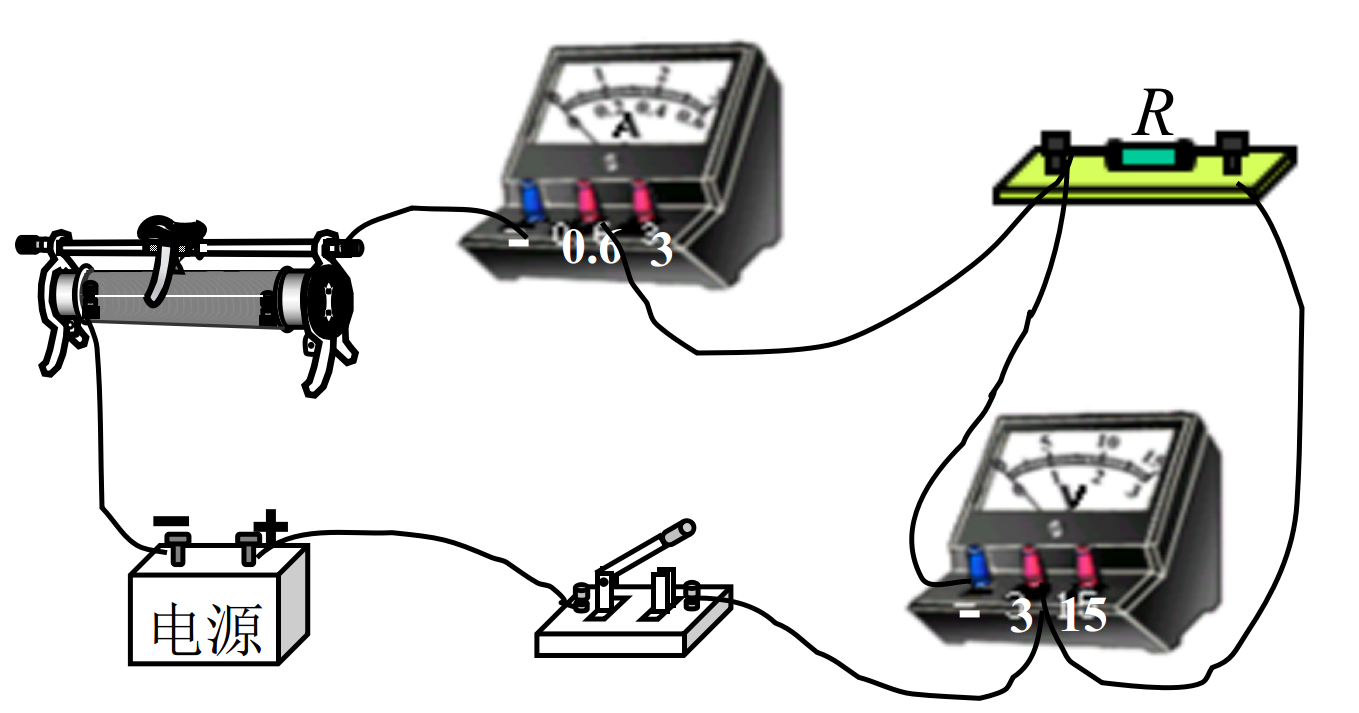
\includegraphics [width=0.7\linewidth ]{picture/screenshot007}
\item a
\item d
\item $ 4.4\sim 4.7 $ 均可,图见下
\item B
\item (2)作图如下: \\ \includesvg [width=0.23\linewidth ]{picture/svg/613}
\item 定值电阻在电路中消耗的功率会超过$ 1/8W $, $ R_{2} $的功率满足实验要求
\item $ 51.0 $ $ (2 $分。在$ 49.053.0 $范围内的均给分)
\item 忽略了电压表的分流(此答案对应于图$ (a) $) 或:忽略了电流表的分压(此答案对应于图$ (b) $ ) $ (2 $分,其他合理答案也给分)
\item ($ 1 $)电路原理图如图$ (a) $所示。$ (5 $分,给出图$ (b) $也给分。原理正确$ 2 $分,仪器选择正确$ 3 $分)\\ \includesvg [width=0.23\linewidth ]{picture/svg/619} \par \par 
\item AC
\item ②如右图示\\ \includesvg [width=0.23\linewidth ]{picture/svg/614}
\item B
\item C
\item F
\item 大于
\item 电压表的读数大于待测电阻两端实际电压(其他正确表述也可)
\item ②实验电路图如答图示\\ \includesvg [width=0.23\linewidth ]{picture/svg/615} \par 
\item $ R_{2} $
\item a
\item $ 2.30 $($ 2.29 $、$ 2.31 $均正确)
\item $ 94 $($ 93 $、$ 95 $均正确)
\item (2)如图所示\\ 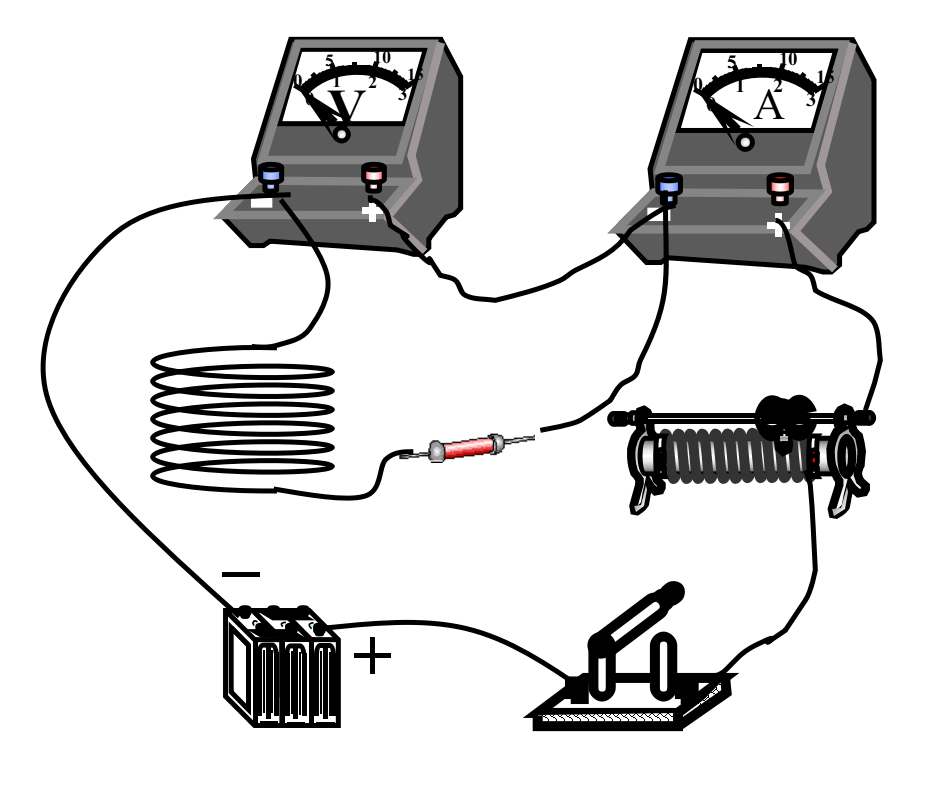
\includegraphics [width=0.5\linewidth ]{picture/screenshot009} \par \par 
\item $ \times $
\item 用“$ \times $”数据点连直线,$ R=(1.1 \sim 1.3) \ \Omega $;用“$ \circ $”数据点连直线,同理得$ R=(1.5 \sim 1.7) \ \Omega $
\item 答题图:\\ 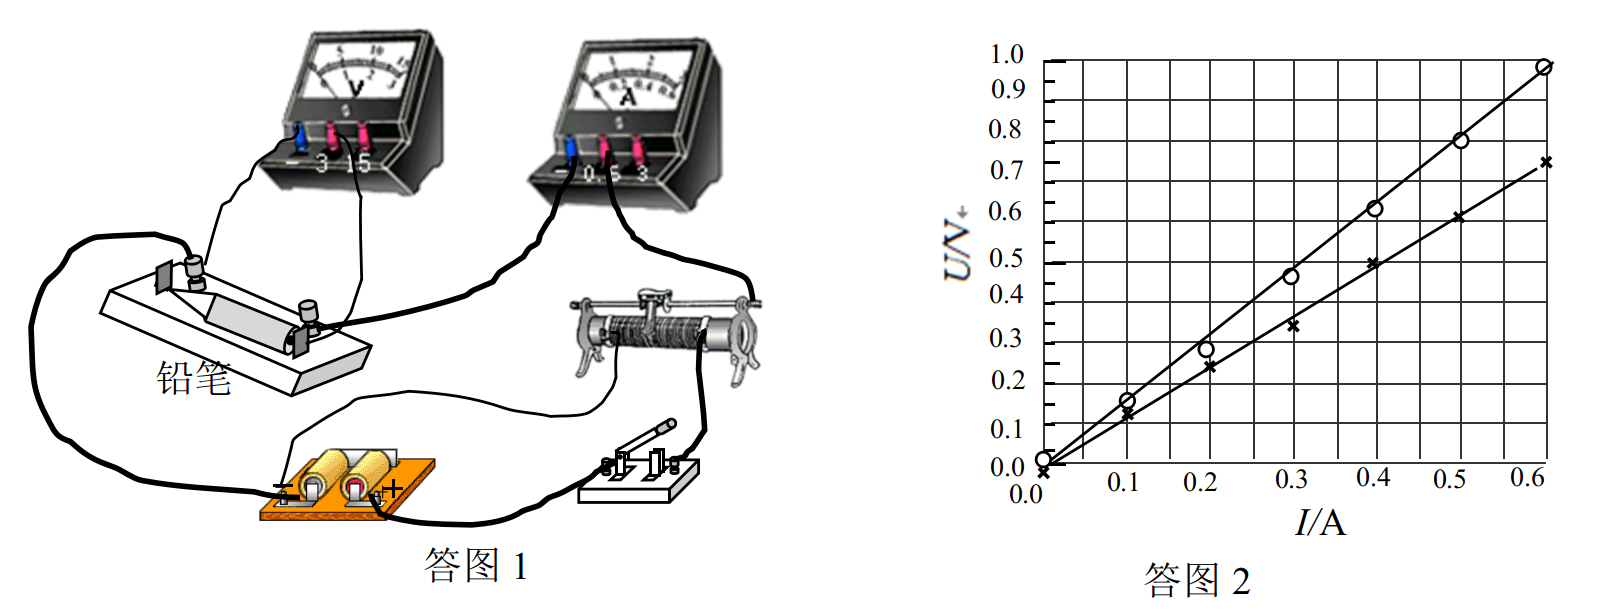
\includegraphics [width=0.8\linewidth ]{picture/screenshot011} \par \par 
\item B
\item C
\item B
\item C
\item 甲
\item 5.2
\item B
\item D
\item A
\item $ (2) $如答图$ 1 $所示:\\ \includesvg [width=0.23\linewidth ]{picture/svg/626} \par 
\item $ 0.58 $ ($ 0.57 $到$ 0.59 $均可)
\item $ 65 $($ 64 $到$ 66 $均可)
\item $ 1 ^{\prime } $ 和$ 2 ^{\prime } $
\item ①电路图如图示\\ \includesvg [width=0.23\linewidth ]{picture/svg/629} \par \par 
\item $ A_{2} $
\item $ R_{2} $
\item 25
\item $\frac { U _ { 0 } } { I _ { 0 } } - r$
\item 相同
\item 相同
\item \begin {enumerate} \item $ 1.773 $ ($ 1.771 \sim 1.775 $均正确) \item $ A_{1} $ \quad $ E_{1} $\\ 电路如图所示 \begin {center} \includesvg [width=0.23\linewidth ]{picture/svg/GZ-3-tiyou-0968} \end {center} \end {enumerate}
\item \begin {enumerate} \item $ 5.01 $ \quad $ 5.315 $ \item 大 \quad 大 \item $ 1280 $ \end {enumerate}
\item \begin {enumerate} \item $ 0.007 \quad 0.638 $ \item 如图所示 \begin {center} \includesvg [width=0.23\linewidth ]{picture/svg/GZ-3-tiyou-0969} \end {center} \end {enumerate}
\item \begin {enumerate} \item $ 0.397 \ mm $ \quad $ (0.395 \sim 0.399) $ \item 甲 \item 如图所示 \begin {center} \includesvg [width=0.23\linewidth ]{picture/svg/GZ-3-tiyou-0974} \end {center} \item $ R_{x}=4.5 \ \Omega $ \quad ($ 4.3 \sim 4.7 $),电路如图 \begin {center} \includesvg [width=0.23\linewidth ]{picture/svg/GZ-3-tiyou-0975} \end {center} \item C \item CD \end {enumerate}
\item \begin {enumerate} \item $ B \quad 0.410 $ \item $ 7 $、$ 9 $ \quad 断路 \item 电流表改为内接;测量多组电流和电压值,计算出电阻的平均值(或多测几组电流值和电压 值,用图象法求电阻值) \end {enumerate}
\item \begin {enumerate} \item C \item 不同 \item 如图所示 \begin {center} \includesvg [width=0.23\linewidth ]{picture/svg/GZ-3-tiyou-0983} \end {center} \item 如图所示 \begin {center} \includesvg [width=0.23\linewidth ]{picture/svg/GZ-3-tiyou-0984} \end {center} \item $ 23.5 $($ 23.0 \sim 24.0 $ 都算对) \end {enumerate}
\item \begin {enumerate} \item $ 0.200 $ \quad $(0.196 \sim 0.204$ 均可 $)$ \item \begin {center} \includesvg [width=0.23\linewidth ]{picture/svg/GZ-3-tiyou-0987} \end {center} \item $\frac {I_{1} R_{1}}{I_{2}-I_{1}}$ \quad 相等 \end {enumerate}
\item \begin {enumerate} \item 如图所示; \begin {center} \includesvg [width=0.23\linewidth ]{picture/svg/GZ-3-tiyou-0989} \end {center} \item 电阻率的允许范围:\\ $\rho _{a}: 0.96 \times 10^{-6} \Omega \cdot m \sim 1.10 \times 10^{-6} \Omega \cdot m$\\ $\rho _{b}: 8.5 \times 10^{-6} \Omega \cdot m \sim 1.10 \times 10^{-7} \Omega \cdot m$\\ $\rho _{c}: 0.96 \times 10^{-6} \Omega \cdot m \sim 1.10 \times 10^{-6} \Omega \cdot m$ \\ 通过计算可知,金属丝$ a $与$ c $电阻率相同,远大于金属丝$ b $的电阻率。 \end {enumerate}
\item $ R_{0} $
\item 标准电流表$ A_{0} $
\item $ R_N $
\item 标准电流表$ A_{0} $的示数仍为 I
\item 平均值
\item $R \frac { U _ { 1 } } { U _ { 2 } }$
\item 200
\item $\left ( \frac { U _ { 2 } } { U _ { 1 } } - 1 \right ) R _ { 0 }$
\item 48.2
\item 实物连线如图示:\\ \begin {figure}[h!] \includesvg [width=0.23\linewidth ]{picture/svg/636} \end {figure}
\item D
\item C
\item 变大
\item $ 31.3 $
\item ③ 关系图线如图:\\ \includesvg [width=0.23\linewidth ]{picture/svg/639} \par 
\item 5.2
\item 148.2
\item $\frac { R _ { 1 } } { E } + \frac { r + R _ { \mathrm { A } } } { E }$
\item 9.1
\item 1.0
\item c
\item d
\item $ > $
\item 小
\item $ R_{1} $
\item 2520
\item D
\item ($ 2 $)连线如下图 \begin {figure}[h!] \centering \includesvg [width=0.23\linewidth ]{picture/svg/645} \end {figure} \par 
\item $ > $
\item 断开$ S_{2} $,调节电阻箱使电压表成半偏状态,电压表所在支路总电阻增大,分得的电压也增大;此时$ R_{0} $两端的电压大于电压表的半偏电压,故$ R ^{\prime } _ V>R_v $
\item (1)实验电路如右图所示: \includesvg [width=0.23\linewidth ]{picture/svg/647} \par \par 
\item ③
\item ⑥
\item 将滑动触头移至最左端
\item 多次移动滑动触头,记录相应的$ G_{1} $、$ G_{2} $读数$ I_{1} $、$ I_{2} $
\item $ r_{1} =(k $-$ 1) R_{1} $
\item ($ 2 $)如图 \includesvg [width=0.23\linewidth ]{picture/svg/650} \par 
\item C
\item AC
\item $ \frac {99}{79} $
\item ($ 1 $)电表改装时,微安表应与定值电阻$ R $并联接入虚线框内,则实物电路连接如下图所示: \par \includesvg [width=0.23\linewidth ]{picture/svg/653} \par \par 
\item $\frac { 1 } { 99 } R _ { g }$
\item 49.5
\item 49.0
\item 黑
\item 10
\item 225
\item 25.0
\item $ 0.780(0.78 $同样给分)
\item $ (1) $如图: \includesvg [width=0.23\linewidth ]{picture/svg/661} \par 
\item 100
\item 910
\item 2000
\item 50
\item M
\item 大于
\item 电流
\item 电压
\item 黑
\item 1.00
\item 880
\item 根据图(a)连线:电流表与$ R_2 $串联、开关与$ R_1 $串联,然后两支路并联分别接表笔A、B。 \includesvg [width=0.23\linewidth ]{picture/svg/659} \par 
\item 100
\item 2910
\item ($ 1 $)如图所示 : \includesvg [width=0.23\linewidth ]{picture/svg/655} \par 
\item $ B $、$ E $、$ F $、$ A $、$ D $、$ C $
\item 相等
\item $\frac { I _ { 1 } } { I - I _ { 1 } } r$
\item 15
\item 35
\item 300
\item 3000
\item C
\item 闭合开关时,若电表指针偏转,则损坏的电阻是$ R_{1} $;若电表指针不动,则损坏的电阻是$ R_{2} $
\item $ 1 $点至$ 4 $点
\item $ 0,30 $
\item $ 0.75 $
\item C
\item 它靠近变阻器左端的接线柱
\item 增加小灯泡两端的电压,记录电流表和电压表的多组读数,直至电压达到额定电压
\item ($ 2 $)电路图如图所示: \includesvg [width=0.23\linewidth ]{picture/svg/667} \par 
\item B
\item B
\item $ 0.1 $
\item 1.40
\item 0.23
\item 非线性
\item ①电路连接如答图$ 1 $所示 : \includesvg [width=0.23\linewidth ]{picture/svg/672} \par $ I_x-U_x $图线 如答图$ 2 $所示 : \includesvg [width=0.23\linewidth ]{picture/svg/674}
\item D
\item 左
\item 1
\item 5
\item 增大
\item 0.10 A
\item 0.24 A
\item 2.00 V
\item 0.27 V
\item ($ 8.3\pm 0.1 $)$ \Omega $
\item ($ 2.7\pm 0.1 $)$ \Omega $
\item 答案如图$ 1 $所示: \includesvg [width=0.23\linewidth ]{picture/svg/679}
\item B
\item ①电路如图: \includesvg [width=0.23\linewidth ]{picture/svg/681}
\item A
\item $ \times 1 $
\item $ a $
\item $ b $
\item ab
\item ②电流表的电阻也就几欧,与电压表几千欧相比,小电珠算小电阻,所以电压表必须外接,伏安特性曲线要求电压从0开始逐渐变大,所以滑动变阻器必须与电压采用分压接法。
\item $U = E - I r$
\item 不变
\item 增大
\item 0.975
\item 480
\item 267
\item ②见题答图 \includesvg [width=0.23\linewidth ]{picture/svg/686}
\item 0.44
\item 4
\item $ 2.22 \sim 2.28 $
\item ①连线如图: 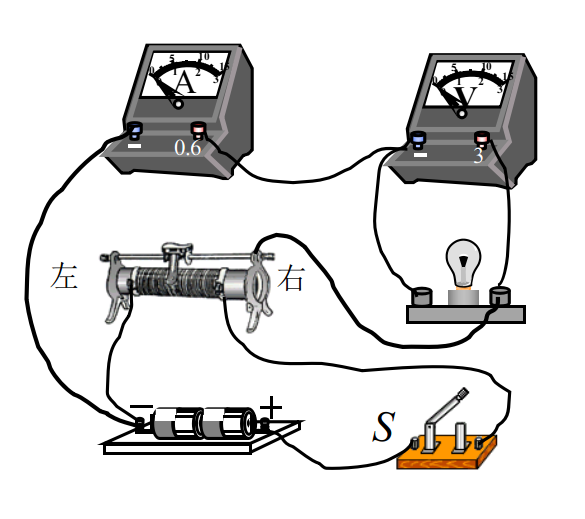
\includegraphics [width=0.7\linewidth ]{picture/screenshot014}
\item 增大
\item 增大
\item 0.39
\item 1.17
\item ($ 1 $)如答图$ 1 $示: \includesvg [width=0.23\linewidth ]{picture/svg/691}
\item 10
\item b
\item 增大
\item Y
\item 3.2
\item 0.50
\item D
\item A
\item $ (0.75\pm 0.10)\ \Omega $
\item 0.22 $\Omega $
\item A
\item C
\item C
\item $ ka $
\item $ k-R_{2} $
\item 80.0
\item 0.00444
\item 1.50
\item (2)如图示 : \includesvg [width=0.23\linewidth ]{picture/svg/695}
\item C
\item 6
\item 7.5
\item 10
\item ②实验原理电路图如图示。 \includesvg [width=0.23\linewidth ]{picture/svg/702}
\item 5
\item 4
\item ③由于电压表量程太小,所以需要改装,将它与$ R_{2} $串联即成为一个量程为$ 4.0V $的新的电压表;电流表$ A_{1} $量程太大,不可用,可以将$ A_{2} $改装:将它并联一个小电阻$ R_{1} $则成为一个量程为$ 0.72A $的新的电流表了。由于灯泡的电阻远小于电压表内阻而与电流表内阻相差不多,属于小电阻,故用电流表外接法比较合适。答案如答图$ 1 $较合适,若用答图$ 2 $则不太合适。 \par \includesvg [width=0.4\linewidth ]{picture/svg/700} \par 说明:画出答图$ 1 $给$ 4 $分,只画出答图$ 2 $给$ 2 $分。
\item 9.4
\item $ 9.5-11.1 $
\item (ⅰ)连接电路如图所示。 (ⅱ)所作图象如图所示 \includesvg [width=0.23\linewidth ]{picture/svg/705}
\item ①开关未断开 ②电阻箱阻值为零
\item $ 1.4 $($ 1.30 \sim 1.44 $都算对)
\item $ 1.2 $($ 1.0 \sim 1.4 $都算对)
\item $ 1.4 $(结果与($ 2 $)问第一个空格一致)
\item $ 1.0 $(结果比($ 2 $)问第二个空格小$ 0.2 $)
\item ($ 2 $)(见下图) : \includesvg [width=0.23\linewidth ]{picture/svg/708}
\item 0.110
\item 9.09
\item 1.0(在$ 0.961.04 $之间均给分)
\item 6.0(在$ 5.9\sim 6.1 $之间均给分)
\item 3.0 V (在$ 2.7\sim 3.3 $之间均给分)
\item $1.0 \ \Omega $(在$ 0.6\sim 1.4 $之间均给分)
\item (3)图线如答图 \includesvg [width=0.23\linewidth ]{picture/svg/712}
\item $ 2.90 $(在$ 2.89 \sim 2.91 $之间均给分)
\item $ 1.02 $(在$ 0.93 \sim 1.13 $之间均给分)
\item $ (1) $连接如答图$ 1 $所示.$ U $­ \lmd {1} 图线如答图$ 2 $所示. \par \includesvg [width=0.23\linewidth ]{picture/svg/715}
\item 甲
\item B
\item C
\item 1.50
\item 0.83
\item C
\item $ (3) $第$ 3 $个点为数据误差,连线时略过,如图: \includesvg [width=0.23\linewidth ]{picture/svg/719}
\item C
\item 2.8
\item 2
\item D
\item 3
\item 0.44
\item $ 1.60 $ $ (1 $. $ 58 $ $ \sim $ $ 1 $. $ 62 $ 都算对)
\item $ 1. 20 $ $ (1 $. $ 18 $ $ \sim $ $ 1 $. $ 26 $ 都算对)
\item 干电池长时间使用后,电动势和内阻会发生变化,导致实验误差增大。
\item (2) $ U-I $ 图线见右图 : \includesvg [width=0.23\linewidth ]{picture/svg/726}
\item 1.0
\item $ 1.66 $
\item 充分利用测得的数据
\item CD
\item ②如答图所示: \includesvg [width=0.23\linewidth ]{picture/svg/722}
\item A
\item D
\item F
\item a
\item d
\item C
\item g
\item f
\item h
\item $ \frac {1}{U} $、$ \dfrac {1}{R} $、$ U $
\item $ \frac {U}{R} $、$ \frac {R}{U} $、$ R $
\item ②为减小误差,电流表应采用内接法,同时注意电表的正、负接线柱,电路图如右图示,故可知导线应连接$ a $ $ d $ 、$ c $ $ g $、 $ f $ $ h $。 \includesvg [width=0.23\linewidth ]{picture/svg/724}
\item 并联
\item 5.0
\item 1.53
\item 2
\item ($ 2 $)①倾斜直线如下图示; \includesvg [width=0.23\linewidth ]{picture/svg/729}
\item $ aa ^{\prime } $
\item $ bb ^{\prime } $
\item $ 1.41 $($ 1.36 \sim 1.44 $均可)
\item ,$ 0.5 $($ 0.4 \sim 0.6 $均可)
\item \begin {enumerate} \item $ 900 $ \quad $ R_{1} $ 连线如图: \begin {center} \includesvg [width=0.23\linewidth ]{picture/svg/GZ-3-tiyou-0993} \end {center} \item $ 45 $ \quad $ 5 $ \item $ 0 $ \quad $ 35000.0 $ \end {enumerate}
\item $ \times 1 $ \quad 乙 \quad ③
\item \begin {enumerate} \item $11.5 \quad (11.2 \sim 11.8)$;蓄电池 \item 小灯 \end {enumerate}
\item \begin {enumerate} \item $ \times 10 $ \quad 欧姆调零 \quad $ 70 $ \item 电路如图;直流电压 $ 10 \ V $ 档 \begin {center} \includesvg [width=0.23\linewidth ]{picture/svg/GZ-3-tiyou-1001} \end {center} \end {enumerate}
\item \begin {enumerate} \item 短接 \item $ 15.0 $ \quad $ 3.60 $ \item $ 12.0 $ \item $ 9.00 $ \quad $ 15.0 $ \end {enumerate}
\item \begin {enumerate} \item $ A $ \item 短暂 \item $ 5.0 \ \Omega $,可能的电路有两种,如图: \begin {center} \includesvg [width=0.23\linewidth ]{picture/svg/GZ-3-tiyou-1010} \end {center} \begin {center} \includesvg [width=0.23\linewidth ]{picture/svg/GZ-3-tiyou-1011} \end {center} \end {enumerate}
\item \begin {enumerate} \item $ R_{1} $ \quad $ R_{1} $ 和 $ R_{2} $ 串联 \quad $ R_{2} $(或电源) \item D \end {enumerate}
\item \begin {enumerate} \item 小 \quad $ 290 $ \item 准确 \end {enumerate}
\item \begin {enumerate} \item ①断开待测电阻,将选择开关旋到“$ \times 10^{0} $”档;\\ ②将两表笔短接,调整“欧姆调零旋钮”,使指针指向“$ 0 \ \Omega $”; \\ ③再接入待测电阻,将指针示数$ \times 100 $,即为待测电阻阻值。 \item 如图所示 \begin {center} \includesvg [width=0.23\linewidth ]{picture/svg/GZ-3-tiyou-1024} \end {center} \item 电阻 \qquad 1、2 \qquad 1 \end {enumerate}
\item \begin {enumerate} \item 黑 \item $ 14.0 \quad 53.0 \quad 4.6 $ \item $ 102 $ \item $ 1.54 $ \end {enumerate}
\item \begin {enumerate} \item $ 5.4 $ \item 小于 \end {enumerate}
\item \begin {enumerate} \item EDBCA \item $ 2.8 \sim 3.0 $ \item B \quad $ 250 \ mA $ \end {enumerate}
\item \begin {enumerate} \item 黑 \item B \item $ 160 \ \Omega \quad 880 \ \Omega $ \item $ 1.49 \ mA $;$ 11.0 \times 10^{0} \ \Omega $;$ 2.95 \ V $ \end {enumerate}
\item \begin {enumerate} \item 左偏 \quad 右偏 \item 不停振动 \item 短接 $ G $ 表前后各摇动 $ G $ 表一次,比较指针偏转,有明显变化,则线圈断了;没有明显偏转则未断。 \end {enumerate}
\item 有 \quad 无 \quad 无
\item \begin {enumerate} \item 顺时针 \item 逆时针 \end {enumerate}
\item \begin {enumerate} \item AD \item 如图 \begin {center} \includesvg [width=0.23\linewidth ]{picture/svg/GZ-3-tiyou-1038} \end {center} \end {enumerate}
\item \begin {enumerate} \item $ 5.00 $ \quad 变小 \quad 增大 \quad $ B $ \item $ 2.8 $ \end {enumerate}
\item \begin {enumerate} \item 前 \item D \end {enumerate}
\item \begin {enumerate} \item 减小 \item $ 1 $ \item $ 5 $ \end {enumerate}
\item 减小 \quad 增大 \quad 控制变量法
\item \begin {enumerate} \item 如下图 \begin {center} \includesvg [width=0.23\linewidth ]{picture/svg/GZ-3-tiyou-1045} \end {center} \item $ 0.6 $ \end {enumerate}
\item \begin {enumerate} \item 如图 \begin {center} 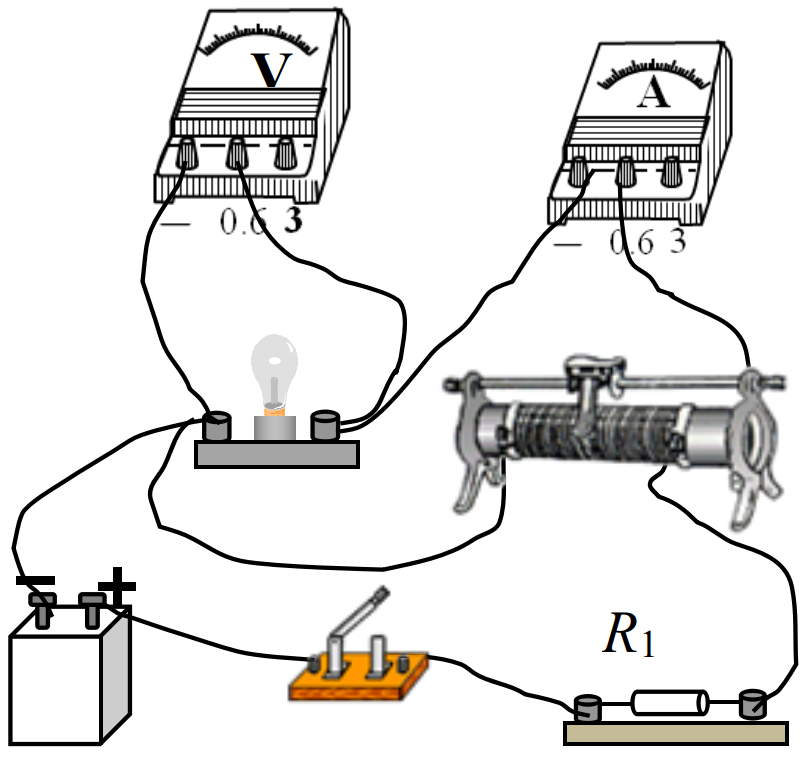
\includegraphics [width=0.7\linewidth ]{picture/screenshot067} \end {center} \item $ 10 $ \item 电池 \item 图线不应画为直线;横坐标的标度不恰当. \end {enumerate}
\item \begin {enumerate} \item $ b $ \item 如图 \begin {center} \includesvg [width=0.23\linewidth ]{picture/svg/GZ-3-tiyou-1051} \end {center} \item $ 450 $ \item $ 620.0 $ \quad $ 33.0 $ \end {enumerate}
\item \begin {enumerate} \item $ M $ \item 如图所示 \quad $ 1.5 $($ 1.4 $ 或 $ 1.6 $) \begin {center} \includesvg [width=0.23\linewidth ]{picture/svg/GZ-3-tiyou-1055} \end {center} \item $ b $ \quad $ c $ \quad $ S_{1} $,$ E $(或 $ S_{2} $,$ E $) \end {enumerate}
\item \begin {enumerate} \item 如图所示 \begin {center} \includesvg [width=0.23\linewidth ]{picture/svg/GZ-3-tiyou-1060} \end {center} \item $ 0.10 $ \item $R_{x}=\frac {L u}{I}$ \quad $R_{x}=k u=6.0 \ \Omega $ \end {enumerate}
\item \begin {enumerate} \item 连线如图示 \begin {center} \includesvg [width=0.23\linewidth ]{picture/svg/GZ-3-tiyou-1062} \end {center} \item \begin {enumerate} \item none \item none \item 重新处于平衡状态\\ 电流表的示数 $ I $\\ 此时细沙的质量 $ m_{2} $ \item $ D $ 的底边长 $ L $ \end {enumerate} \item $B=\frac {\left |m_{1}-m_{2}\right | g}{I L}$ \item $m_{2}>m_{1}$ \end {enumerate}
\item \begin {enumerate} \item 如图所示 \begin {center} \includesvg [width=0.23\linewidth ]{picture/svg/GZ-3-tiyou-1069} \end {center} \item $ 0.37 $(或 $ 0.36 $) \item BC \end {enumerate}
\item \begin {enumerate} \item 如图 \begin {center} \includesvg [width=0.23\linewidth ]{picture/svg/GZ-3-tiyou-1072} \end {center} \item $ 20 $($ 19 \sim 21 $ 都算对) \item 偏小\\ 改变滑动变阻器阻值,使电压表示数为$ 1.50 \ V $ \end {enumerate}
\item \begin {enumerate} \item $ 1.30 $ \item A \item B \item 短路 \end {enumerate}
\item \begin {enumerate} \item $ c $ \item $ 4.1 $ ($ 4.0 \sim 4.2 $) \item 减小 \quad $ M $ \item $ b $ \quad $ d $ \end {enumerate}
\item \begin {enumerate} \item 如答图示 \begin {center} \heiti \includesvg [width=0.23\linewidth ]{picture/svg/GZ-3-tiyou-1084} \end {center} \item $ 3.6 \ V $ \item $ U-I $图像如图 \quad $ 40 \ s $ \begin {center} \includesvg [width=0.23\linewidth ]{picture/svg/GZ-3-tiyou-1083} \end {center} \item 使实验前电容器两极板上的电荷相中和 \end {enumerate}
\item \begin {enumerate} \item 如下图 \begin {center} \includesvg [width=0.23\linewidth ]{picture/svg/GZ-3-tiyou-1086} \end {center} \item $ R_{2} $ \item \begin {enumerate} \item $ 650.0 $ \item $ b $\\ 接通电源后,流过报警器的电流会超过 $ 20 \ mA $,报警器可能损坏坏 \item $ c $ \quad 报警器开始报警 \end {enumerate} \end {enumerate}
\item \begin {enumerate} \item 如图所示 \begin {center} \includesvg [width=0.23\linewidth ]{picture/svg/GZ-3-tiyou-1088} \end {center} \item AC \end {enumerate}
\item \begin {enumerate} \item A \item ①②③(或①③②) \item 如图 \quad $ 0.04t+8.8 (0.04t+8.6 \sim 0.04t+9.0 $ 都算对) \begin {center} \includesvg [width=0.23\linewidth ]{picture/svg/GZ-3-tiyou-1091} \end {center} \end {enumerate}
\item \begin {enumerate} \item 连线见答图所示 \begin {center} \includesvg [width=0.23\linewidth ]{picture/svg/GZ-3-tiyou-1094} \end {center} \item \begin {enumerate} \item $ 20 $ \item 左 \item 相等 \item $ 2250 $ \end {enumerate} \item 调节 $ R_{1} $ 上的分压,尽可能使微安表接近满量程 \end {enumerate}
\item \begin {enumerate} \item $ E_{2} $ \quad $ R_{2} $ \item $ C $ \item 不偏转 \quad 偏转 \item ⑤④②③① \end {enumerate}
\item \begin {enumerate} \item ACE \quad $ n_{b} $ \item $ b $ 到 $ a $ \quad A \end {enumerate}
\item C
\item BD
\item D
\item D
\item C
\item B
\item C
\item C
\item C
\item ABC
\item C
\item CD
\item 引力
\item C
\item A
\item C
\item B
\item \begin {enumerate} \renewcommand {\labelenumi }{\arabic {enumi}.} \item 插入后压强$p = p _ { 0 } L _ { 0 } / L ^ { \prime } = 62.5 \mathrm { cm } \mathrm { Hg }$. \item 管口距槽内水银面距离距离$H = L - L ^ { \prime } - h ^ { \prime } = 27.5 \mathrm { cm }$. \par \par \par \end {enumerate}
\item A
\item B
\item $ W=1500\ J $
\item A
\item A
\item $P _ { 3 } = \frac { H _ { 1 } } { H _ { 3 } } P _ { 0 }$ \qquad $T _ { 0 } = \frac { H _ { 3 } } { H _ { 2 } - H _ { 3 } } \Delta T$.
\item BD
\item $V _ { A } = \frac { 7 } { 6 } V _ { 0 }$, \qquad $T _ { A } = 1.4 T _ { 0 }$.
\item a
\item C
\item \begin {enumerate} \renewcommand {\labelenumi }{\arabic {enumi}.} \item $T _ { 2 } = \frac { p _ { 2 } V _ { 2 } } { p _ { 1 } V } T _ { 1 } = \frac { 66 \times 25 } { 60 \times 22 } \times 280 \mathrm { K } = 350 \mathrm { K }$ \item $l = 10\ \mathrm { cm }$ \par \par \par \end {enumerate}
\item \begin {enumerate} \renewcommand {\labelenumi }{\arabic {enumi}.} \item 2 \item $ \dfrac {V_{1} ^{\prime } }{V_{2} ^{\prime } } = \dfrac { 5 }{ 4 } $ \par \par \par \end {enumerate}
\item 0.1
\item 360
\item 减小
\item 偏低
\item \begin {enumerate} \renewcommand {\labelenumi }{\arabic {enumi}.} \item 不正确, 水银柱向上移动 \item $\Delta p _ { A } = \Delta p _ { B }$ \par \par \par \end {enumerate}
\item B
\item AC
\item A
\item B
\item A
\item C
\item AB
\item AD
\item A
\item B
\item AC
\item C
\item AD
\item AB
\item \begin {enumerate} \item ②在量筒中滴入$ N $滴溶液,\\ ③在水面先撒上痱子粉。 \item $ 1.2 \times 10^{-9} $ \end {enumerate}
\item \begin {enumerate} \item ④①②⑤③ \item $ 5 \times 10^{-10} \ m $ \end {enumerate}
\item \begin {enumerate} \item $p_{0}\left (V_{0}+\Delta V\right )=\left (p_{0}+\Delta p_{1}\right ) V_{0}$\\ $p_{0} V_{0}=\left (p_{0}-\Delta p_{2}\right )\left (V_{0}+\Delta V\right )$ \item $ 560 $ \quad $ 9.58 \times 10^{4} $ \item A \end {enumerate}
\item \begin {enumerate} \item 向下 \\ $ B $、$ C $ 两管内水银面等高 \item A \end {enumerate}
\item \begin {enumerate} \item A \item BC \item 偏大;调整两管液面高度差,使右管液面比左管液面高 $ 1 \ cm $,然后读数 \end {enumerate}
\item B
\item $n=5 \times 10^{16}$
\item C
\item C
\item AD
\item BC
\item B
\item AC
\item BD
\item A
\item CD
\item B
\item B
\item B
\item D
\item B
\item BD
\item A
\item C
\item B
\item A
\item C
\item D
\item BC
\item A
\item BC
\item A
\item B
\item B
\item A
\item B
\item C
\item D
\item D
\item D
\item C
\item C
\item B
\item B
\item A
\item D
\item \ce {_{27}^{60}Co \rightarrow { }_{28}^{60}Ni + _{-1}^{60}e} \quad $h\left (\nu _{1}+\nu _{2}\right )$
\item D
\item D
\item B
\item \begin {enumerate} \item \ce {_{Z}^{A}X \rightarrow ^{A-4}_{Z-2}Y + _{2}^{4}He} \item $I=\frac {q^{2} B}{2 \pi m} \quad T=\frac {2 \pi m}{q B}$ \item $\Delta m=\frac {(M+m) q^{2} B^{2} R^{2}}{2 m M c^{2}}$ \end {enumerate}
\item D
\item D
\item B
\item D
\item B
\item AC
\item C
\item AD
\item D
\item ${ }_{84}^{210} \mathrm {Po} \rightarrow { }_{82}^{206} \mathrm {~Pb}+{ }_{2}^{4} \mathrm {He}$\\ ${ }_{2}^{4} \mathrm {He}+{ }_{9}^{19} \mathrm {~F} \rightarrow { }_{10}^{22} \mathrm {Ne}+{ }_{1}^{1} \mathrm {H}$
\item AC
\item C
\item C
\item AD
\item B
\item A
\item B
\item B
\item BD
\item 中子 \quad 核裂变
\item B
\item D
\item AC
\item C
\item A
\item B
\item B
\item C
\item B
\item D
\item C
\item BD
\item AC
\item 
\item ABC
\item \begin {enumerate} \item $L+\frac {m g \sin \alpha }{k}$ \item $F_{\text {合 }}=-k x,$ 可知物块作简谐振动。 \item $\frac {L}{4}+\frac {2 m g \sin \alpha }{k}$ \item $\mu \geq \frac {(k L+4 m g \sin \alpha ) \cos \alpha }{4 M g+4 m g \cos ^{2} \alpha -k L \sin \alpha }$ \end {enumerate}
\item $ 0.785 $ \quad $ 0.08 $
\item B
\item C
\item $d=R-k^{2} R$
\item A
\item A
\item D
\item A
\item B
\item C
\item AD
\item D
\item A
\item B
\item C
\item D
\item D
\item B
\item ABD
\item C
\item B
\item C
\item ABD
\item C
\item D
\item D
\item CD
\item BCD
\item C
\item AB
\item C
\item C
\item CD
\item D
\item C
\item D
\item A
\item BD
\item AD
\item C
\item A
\item D
\item D
\item B
\item AC
\item D
\item $ 5 $ \quad $ 7/9 $
\item D
\item 衍射 \quad 接近
\item B
\item BD
\item B
\item AD
\item $ 2 $ \quad $ 0 $
\item B
\item C
\item CD
\item BC
\item B
\item A
\item B
\item C
\item C
\item B
\item B
\item A
\item A
\item C
\item D
\item D
\item D
\item B
\item B
\item A
\item D
\item B
\item C
\item C
\item B
\item D
\item A
\item B
\item C
\item A
\item $ \theta =60 \degree $
\item D
\item A
\item C
\item AD
\item C
\item 衍射 \quad 波动说
\item 减小;光的波长比障碍物小得多
\item D
\item B
\item AC
\item C
\item B
\item BD
\item D
\item D
\item AB
\item \begin {enumerate} \item $ 0.996 \sim 1.000 $ \quad $ a $ \item $ \frac {D \lambda }{2h} $ \quad 不能 \end {enumerate}
\item A
\item B
\item $n=5 \times 10^{16}$
\item C
\item C
\item AD
\item BC
\item B
\item AC
\item BD
\item A
\item CD
\item B
\item B
\item B
\item D
\item B
\item C
\item ABD
\item AB
\item CD
\item C
\item ACD
\item C
\item \begin {enumerate} \item $U_{m}=\frac {E_{K m}}{e}$ \quad $I_{\text {短 }}=N e$ \item $E=U_{m}=\frac {E_{K m}}{e}$ \quad $r=\frac {E_{K m}}{N e^{2}}$ \item 设单位时间内到达 $B$ 板的电子数为 $N^{\prime },$ 则电路中的电流 \begin {equation}\label {key} I=\frac {Q^{\prime }}{t}=\frac {N^{\prime } t e}{t}=N^{\prime } e \end {equation} 则外电阻消耗的功率 \begin {equation}\label {key} P=U I=U N^{\prime } e \end {equation} 光电子在两极板中运动时,两极板间电压为 $U,$ 每个电子损失的动能 \begin {equation}\label {key} \Delta E_{K \text { 每个 }}=e U \end {equation} 则单位时间内到达 $B$ 板的电子损失的总动能 \begin {equation}\label {key} \Delta E=N^{\prime } \Delta E_{K \text { 每个 }}=N^{\prime } e U \end {equation} 因此 $P=\Delta E_{K}$。 \end {enumerate}
\item D
\item B
\item C
\item 玻璃砖直角边绕$ O $点旋转过的角度$ \theta $ \quad $ \frac {1}{\sin \theta } $
\item \begin {enumerate} \item 解析如图 \begin {center} \includesvg [width=0.83\linewidth ]{picture/svg/GZ-3-tiyou-1470} \end {center} \item $ n=1.51 $ \item $ A $ \end {enumerate}
\item 光学 \quad $ d $ \quad $ e $
\item \begin {enumerate} \item AD \item D \item $ \frac {AC}{BD} $ \end {enumerate}
\item C
\item \begin {enumerate} \item A \item $ 1.970 \ mm $ \end {enumerate}
\item D
\item B
\item C
\item D
\item $ J \cdot s $ \quad $ kg \cdot m^{2}/s $
\item B
\item A
\item A
\item B
\item AC
\item ABD
\item ABD
\item BCD
\item AD
\item ACD
\item AB
\item A
\item C
\item B
\item B
\item C
\item D
\item B
\item 使油酸在浅盘的水面上容易形成一块单分子层油膜
\item 把油酸酒精溶液一滴一滴地滴入小量筒中,测出$ 1mL $油酸酒精溶液的滴数,得到一滴溶液中纯油酸的体积
\item 油膜稳定后的表面积$ S $
\item \begin {enumerate} \renewcommand {\labelenumi }{\arabic {enumi}.} \item $ 41 \ cm $; \item $ 312K $ \par \par \par \end {enumerate} \par \par 
\item 低于
\item 大于
\item \begin {enumerate} \renewcommand {\labelenumi }{\arabic {enumi}.} \item $3.2 \times 10 ^ { 7 } \mathrm { Pa }$ \item $1.6 \times 10 ^ { 8 } \mathrm { Pa }$ \par \par \par \end {enumerate} \par \par 
\item 大于
\item 等于
\item 大于
\item \begin {enumerate} \renewcommand {\labelenumi }{\arabic {enumi}.} \item $\frac { 1 } { 2 } \left ( p _ { 0 } + p \right )$ \item $\frac { 1 } { 2 } p _ { 0 } + \frac { 1 } { 4 } p ; \quad \frac { 4 \left ( p _ { 0 } + p \right ) V _ { 0 } } { 2 p _ { 0 } + p }$ \par \par \par \end {enumerate} \par \par 
\item A
\item 大于
\item 等于
\item $ 138.6\ J $
\item BD
\item $p = 3.2 \times 10 ^ { 4 } \mathrm { Pa }$
\item BDE
\item $m = \frac { 15 p _ { 0 } S } { 26 g }$
\item BDE
\item \par $T_{2}=\left (1+\frac {h}{H}\right )\left (1+\frac {m g}{p_{0} S}\right ) T_{0}$\\ $W = \left ( p _ { 0 } S + m g \right ) h$
\item BCD
\item 两边气柱长度的变化量大小相等$l _ { 1 } ^ { \prime } - l _ { 1 } = l _ { 2 } - l _ { 2 } ^ { \prime }$,$l _ { 1 } ^ { \prime } = 22.5 \mathrm { cm } \quad l _ { 2 } ^ { \prime } = 7.5 \mathrm { cm }$
\item ABC
\item \begin {enumerate} \renewcommand {\labelenumi }{\arabic {enumi}.} \item $V_{1}=\frac {V}{2}$ \qquad $p_{1}=2 p_{0}$ \item 活塞上升直到B的顶部 \item $p_{3}=1.6 p_{0}$ \par \par \end {enumerate} \par \par 
\item ABD
\item \begin {enumerate} \renewcommand {\labelenumi }{\arabic {enumi}.} \item $\frac { \rho _ { 0 } g V T _ { 0 } } { T _ { b } }$ \item $\frac { \rho _ { 0 } g V T _ { 0 } } { T _ { a } }$ \item $\frac { \rho _ { 0 } V T _ { 0 } } { T _ { b } } - \frac { \rho _ { 0 } V T _ { 0 } } { T _ { a } } - m _ { 0 }$ \par \par \par \end {enumerate} \par \par 
\item ABD
\item \begin {enumerate} \renewcommand {\labelenumi }{\arabic {enumi}.} \item $p _ { x } = \frac { \pi \rho g d ^ { 2 } h ^ { 2 } } { 4 V _ { 0 } + \pi d ^ { 2 } ( l - h ) }$ \item $p _ { m } = \frac { \pi \rho g d ^ { 2 } l ^ { 2 } } { 4 V _ { 0 } }$ \par \par \par \end {enumerate} \par \par 
\item BC
\item 甲
\item 乙
\item 摩尔体积$V = \frac { 4 } { 3 } \pi r ^ { 3 } N _ { A }$(或$V = ( 2 r ) ^ { 3 } N _ { A }$),得 $\rho = \frac { 3 M } { 4 \pi r ^ { 3 } N _ { A } }$(或$\rho = \frac { M } { 8 r ^ { 3 } N _ { A } }$),$\rho = 1 \times 10 ^ { 3 } \mathrm { kg } / \mathrm { m } ^ { 3 }$(或$\rho = 0.5 \times 10 ^ { 3 } \mathrm { kg } / \mathrm { m } ^ { 3 }$)
\item ABE
\item $ 1\ cm $
\item BDE
\item \begin {enumerate} \renewcommand {\labelenumi }{\arabic {enumi}.} \item $\Delta p = \frac { 2 \times 0.070 } { 5 \times 10 ^ { - 3 } } \mathrm { Pa } = 28 \mathrm { Pa }$ \item $\frac { r _ { 2 } } { r _ { 1 } } = \sqrt [ 3 ] { 2 } \approx 1.3$ \par \par \par \end {enumerate} \par \par 
\item ABE
\item $ N=4 $(天)
\item CDE
\item $ h=9.42\ m $
\item AC
\item 不变
\item ①
\item $ 8\ J $
\item ABE
\item $V _ { 1 }: V _ { 2 } = 1: 1$
\item BCD
\item \begin {enumerate} \renewcommand {\labelenumi }{\arabic {enumi}.} \item $T _ { 2 } = 330 \mathrm { K }$ \item $p _ { 2 } = 1.01 \times 10 ^ { 5 } \mathrm { pa }$ \par \par \end {enumerate} \par \par 
\item ACD
\item \begin {enumerate} \renewcommand {\labelenumi }{\arabic {enumi}.} \item $ l_{A}=12.0 \ cm $ \item $ \Delta h =13.2\ cm $ \par \par \end {enumerate} \par \par 
\item B
\item C
\item D
\item $\frac { T _ { 2 } } { T _ { 1 } } P _ { 1 } - P _ { 0 }$
\item AD
\item 增大
\item 不变
\item 包装袋漏气。
\item BC
\item \begin {enumerate} \renewcommand {\labelenumi }{\arabic {enumi}.} \item $p _ { 1 } = \frac { T _ { 1 } } { T _ { 0 } } p _ { 0 } = 1.01 p _ { 0 }$ \item $F _ { \min } + p _ { 2 } S = m g + p _ { 0 } S$,$F _ { \min } \approx 0.02 p _ { 0 } S$. \par \par \par \end {enumerate} \par \par 
\item $n = \frac { 4 \pi R ^ { 2 } P _ { 0 } N _ { A } } { M g }$
\item $a = \sqrt [ 3 ] { \frac { M g h } { P _ { 0 } N _ { A } } }$
\item $\Delta h = \frac { 2 P _ { 0 } S + 3 m g } { \left ( P _ { 0 } S + m g \right ) S } - \frac { 2 V } { S }$
\item ADE
\item $\frac {9 m g h T}{4 p T_{0}}$
\item BCE
\item \begin {enumerate} \item $ 320 \ K $ \item $ \frac { 4 }{ 3 } P_{0} $ \end {enumerate}
\item B
\item $\frac {V_{0}}{V} P_{0} S$
\item \begin {enumerate} \item AD \item 增大 \quad 等于 \item $ 5 \times 10^{24} $(或 $ 6 \times 10^{24} $) \end {enumerate}
\item AB
\item \begin {enumerate} \item $ V_{1}=2.5 \ m^{3} \quad h_{2}=10 \ m $ \end {enumerate}
\item CE
\item $m=\frac {4 p_{10} S}{5 g}$
\item D
\item C
\item BCE
\item \begin {enumerate} \item $T=\frac {7}{5} T_{0}$ \item \begin {equation}\label {key} 6 V_{x}^{2}-V_{0} V_{x}-V_{0}^{2}=0 \end {equation} 其解为 $V_{x}=\frac {1}{2} V_{0}, \quad $ 另一个解 $V_{x}=-\frac {1}{3} V_{0},$ 不符合题意,舍去。 \end {enumerate}
\item ABE
\item $ \Delta l =15.0 \ cm $
\item B
\item $\Delta V=\frac {-\Delta p V_{0}}{p_{0}+\Delta p}$
\item \begin {enumerate} \item C \item $ B \rightarrow C $ \item $ n=4 \times 10^{25} \ m^{3} $ \end {enumerate}
\item C
\item \begin {enumerate} \item $ 2.8 \times 10^{-2} \ m^{3} $ \item 放热 \quad 大于 \end {enumerate}
\item ACD
\item $p=\frac {15}{8} l$
\item C
\item ACE
\item \begin {enumerate} \item $ 180 \ mm Hg $ \item $ 364 \ K $ \end {enumerate}
\item AB
\item \begin {enumerate} \item $ 50 \ cm Hg $ \item 作正功 \quad 吸热 \end {enumerate}
\item AB
\item 平均动能 \quad 小于
\item 等压变化 $\frac {V_{A}}{T_{A}}=\frac {V_{B}}{T_{B}},$ 对外做的功 $W=p\left (V_{B}-V_{A}\right )$,根据热力学第一定律 $\Delta U=Q-W$,解得 $\Delta U=5.0 \times 10^{2} \ J$
\item D
\item A
\item ACE
\item $a=\frac {p_{0} S d}{m(L-d)}$
\item ADE
\item 向下时,$ l=12 \ cm $;转回原来位置时,$ l=9.2 \ cm $
\item B
\item D
\item BC
\item $p_{1}=\frac {\rho g h\left (V_{1}+V_{2}\right )+p_{0} V_{1}}{V_{1}}$
\item AD
\item \begin {enumerate} \item $ 364 \ K $ \item 增大 \quad 吸热 \end {enumerate}
\item D
\item 增大; $ Q- p_{0} ( V_{2} - V_{1} ) $
\item BDE
\item \begin {enumerate} \item $ \sqrt {3} $ \item $\sin i^{\prime }=\frac {\sqrt {3}-\sqrt {2}}{2}$ \end {enumerate}
\item CDE
\item \begin {enumerate} \item $ 7 \ m $ \item $ 5.5 \ m $ \end {enumerate}
\item A
\item \begin {enumerate} \item B \item $\frac {\Delta x \cdot d}{(n-1) l}$ \item $ 630 $ \end {enumerate}
\item AD
\item A \quad A
\item $ v=2 \ m/s $ \quad $ \lambda =0.8 \ m $
\item AB
\item $r=\frac {\sqrt {3}+1}{2} R$
\item $ \sqrt {3} $ \quad 大于
\item \begin {enumerate} \item $ v=18 \ cm /s $ ;波沿 $ x $ 轴负方向传播 \item $ x=9 \ cm $ \end {enumerate}
\item $ 365 \quad \frac {245}{17} $
\item \begin {enumerate} \item $\delta =60^{\circ }$ \item $\frac {2 \sqrt {3}}{3} \leq n<2$ \end {enumerate}
\item ACE
\item $ n=\sqrt {3} $
\item $ 2 \ m $ \quad 减弱 \quad 加强
\item $n=\sqrt {2.05} \approx 1.43$
\item ACD
\item $ n=1.55 $
\item BCE
\item \begin {enumerate} \item $d_{M}=\frac {2}{3} R$ \item $d=\frac {3(2 \sqrt {2}+\sqrt {3})}{5} R$ \end {enumerate}
\item AC
\item 频率 \quad 不变
\item $\alpha =30^{\circ }$
\item ACD
\item \begin {enumerate} \item $ 0.05 \ s $ \item 极大的 $ x $ 坐标 $ x=2 \ m $、$ 3 \ m $、$ 4 \ m $; \\ 极小的 $ x $ 坐标 $ x=1.5 \ m $、$ 2.5 \ m $、$ 3.5 \ m $、$ 4.5 \ m $ \end {enumerate}
\item ACE
\item \begin {enumerate} \item $ \sqrt {7} $ \item 示意图 \begin {center} \includesvg [width=0.23\linewidth ]{picture/svg/GZ-3-tiyou-1548} \end {center} 设 $|B E|=x \ m,$ 得 \begin {equation}\label {key} \tan \alpha =\frac {|A Q|}{|Q E|}=\frac {3-x}{\sqrt {7}} \end {equation} 代入数据得: $x=3-\frac {3}{23} \sqrt {161}$ , 由几何关系得,救生员到池边水平距离为 $(2-x) \ m \approx 0.7 \ m$ \end {enumerate}
\item ABC
\item \begin {enumerate} \item $ T=4 \ s \quad v= 7.5 \ cm/s \quad \lambda = 30 \ cm $ \item $y=0.08 \cos \left (\frac {\pi t}{2}+\frac {\pi }{3}\right )$ \end {enumerate}
\item BDE
\item $ 150 \degree $
\item B
\item 频率 \quad $ C $
\item $1.178 \times 10^{-2} \ m$
\item ABD
\item $O E=\frac {\sqrt {2}}{2} R$
\item $ > \quad 0.300 $
\item \begin {enumerate} \item $x=(50+300 n) \ cm \quad (n=0,\pm 1,\pm 2, \pm 3 \ldots \ldots )$ \item $ 0.1 \ s $ \end {enumerate}
\item ABD
\item \begin {enumerate} \item $ PQ=133 \ cm $ \item $ s=125 \ cm $ \end {enumerate}
\item A
\item $ v=2.5 \ m/s $ \quad ;$ P $ 点沿 $ y $ 轴正向振动
\item BC
\item $ 1.5 $ \quad 不容易
\item $n=\frac {\sqrt {449}}{14} \quad $ (或 $\left .n \approx 1.5\right )$
\item AB
\item $\Delta x=R\left (\frac {1}{\sqrt {n^{2}-1}}-\frac {\sqrt {n^{2}-\sin ^{2} i_{0}}}{\sin i_{0}}\right )$
\item BDE
\item $ OE=R \sin r $
\item ACE
\item \begin {enumerate} \item $d=\sqrt {2} R$ \item 右侧与 $O$ 相距 $\frac {\sqrt {3}}{2} R$ \end {enumerate}
\item BCE
\item $\left .n=\sqrt {1+\left (\frac {h}{R-r}\right .}\right )^{2}$
\item D
\item $T=\frac {2 x_{0}}{v} \quad A=\frac {y_{1}-y_{2}}{2}$
\item B
\item ①应从单摆运动到最低点开始计时时,此位置容易判断,计时误差较小 \\ ②为了减小偶然 误差,可以多次测量多次全振动的时间,然后取平均值求周期。
\item 在鳞片中传播的时间$t_{1}=\frac {2 n^{2} d}{c \sqrt {n^{2}-\sin ^{2} i}}$\\ 在空气中传播的时间 $t_{2}=\frac {2 h}{c \cos i}$\\ $t=t_{1}+t_{2}=\frac {2 n^{2} d}{c \sqrt {n^{2}-\sin ^{2} i}}+\frac {2 h}{c \cos i}$
\item AB
\item \begin {enumerate} \item $ i=45 \degree $ \item $t=\frac {\sqrt {6}+\sqrt {2}}{2 c} L$ \end {enumerate}
\item BC
\item $H=\sqrt {\frac {l_{2}^{2}-l_{1}^{2}}{l_{1}^{2}+h^{2}}} l_{3}$
\item ACD
\item \begin {enumerate} \item $\sin i \leq \sqrt {n^{2}-1}$ \item $t_{\max }=\frac {L n^{2}}{c}$ \end {enumerate}
\item $ < $ \quad $ < $
\item \begin {enumerate} \item $ n=\sqrt {3} $ \item $ AC $ 边没有光线透出,分析略 \end {enumerate}
\item C
\item $n=\frac {\sin i}{\sin (i-\alpha )}$
\item A
\item 大于 \quad $ c $(或光速)
\item $n=\frac {1}{\sin 22.5^{\circ }}$
\item \begin {enumerate} \item $ 1 \ m $ \item 加强 \end {enumerate}
\item \begin {enumerate} \item $ 45 \degree $ \item $\frac {4}{3} \sqrt {3} $ \end {enumerate}
\item BDE
\item 光路图见图: \begin {center} \includesvg [width=0.23\linewidth ]{picture/svg/GZ-3-tiyou-1586} \end {center} $d_{2}-d_{1}=L\left (\frac {n_{2}}{\sqrt {4-n_{2}^{2}}}-\frac {n_{1}}{\sqrt {4-n_{1}^{2}}}\right )$
\item 正向 \quad $ 0.8 \ m $
\item $\frac {S^{\prime }}{S}=\frac {\pi }{4}$
\item \begin {enumerate} \item $ v=1 \ m/s $ \item $y=0.2 \sin (0.5 \pi t) \ m$ \end {enumerate}
\item \begin {enumerate} \item $ n=\sqrt {3} $ \item $d=\frac {\sqrt {3}}{3} R$ \end {enumerate}
\item C
\item 挡住 $ C $ 及 $ A $、$ B $ 的像;$ 1.8 $($ 1.6 \sim 1.9 $ 都算对)
\item $ x=1260 \ km $ \quad $ \lambda =4.2 \ km $
\item \begin {enumerate} \item $ 20 $ \item $ -6 $ \end {enumerate}
\item $0<\theta <45^{0}$
\item ABE
\item \begin {enumerate} \item $ 15 \degree $ \item $n=\frac {\sqrt {6}+\sqrt {2}}{2}$ \end {enumerate}
\item CD
\item \begin {enumerate} \item $ \frac { 4 }{ 3 } $ \item $ 3.3 \ m $ \end {enumerate}
\item \begin {enumerate} \item 正 \item $ 100 \ m/s $ \end {enumerate}
\item \begin {enumerate} \item $ \sqrt {3} $ \item 不能 \end {enumerate}
\item C
\item $ 60 \degree $ \quad $ \frac {\sqrt {3}}{3}c $
\item $T=2 \pi \sqrt {\frac {m}{k}}$
\item B
\item $ \frac {hc}{\lambda _{0}} $ \quad $ 1:2 $
\item $I_{F}=\bar {F} t=2 m v+m g t$
\item BC
\item 小于 \quad $ 2:1 $
\item $\frac {m_{1}}{m_{2}}=\frac {3}{2_{1}}$
\item ACE
\item \begin {enumerate} \item 喷泉单位时间内喷出的水的质量为$\frac {\Delta m}{\Delta t}=\rho \cdot v_{0} \cdot S$ \item $h=\frac {v_{0}^{2}}{2 g}-\frac {M^{2} g}{2 \rho ^{2} v_{0}^{2} S^{2}}$ \end {enumerate}
\item $ C \quad AB \quad E \quad F $
\item \begin {enumerate} \item $ 20 \ kg $ \item 不能 \end {enumerate}
\item ABE
\item $\frac {v_{0}^{2}}{2 g l} \geq \mu \geq \frac {32 v_{0}^{2}}{113 g l}$
\item A
\item $ \frac {h\nu }{c} $ \quad $ 2\frac {h\nu }{c} $
\item 钠、钾、铷能发生光电效应
\item ACD
\item \begin {enumerate} \item $k_{0}=2.04 \times 10^{-3} \ s^{2} / m$ \item $\delta =6 \%$ \end {enumerate}
\item $ ek $ \quad $ -eb $
\item $(\sqrt {5}-2) M \leq m<M$
\item ACD
\item \begin {enumerate} \item $\frac {m_{1}}{m_{2}}=\frac {1}{8}$ \item $\frac {W}{\Delta E}=\frac {1}{2}$ \end {enumerate}
\item B
\item D
\item AB
\item $ 3 $ \quad 大于
\item AC
\item $v_{ \text {共} }=\frac {\sqrt {21}}{16} v_{0}$
\item $ 10 \ eV $ \quad $ 10 $
\item $\Delta E_{k}=\left (M-m_{1}-m_{2}\right ) c^{2}, \quad \frac {M}{M-m_{2}}\left (M-m_{1}-m_{2}\right ) c^{2}$
\item BCD
\item \begin {enumerate} \item $ v_{1}=4 \ m/s $ \item $ h ^{\prime } =0.75 \ m $ \end {enumerate}
\item ACE
\item $\delta _{1}=1.7 \%<5 \%$,本实验在允许的误差范围内验证了动量守恒定律。
\item A
\item $ ^{4}_{2}He $ ($ \alpha $ ) \qquad $ 15.2 $
\item $\frac {17}{48} v_{0}, \quad \frac {31}{24} v_{0}$
\item CD
\item \begin {enumerate} \item $ m/2 $ \item $ \frac { 1 }{ 6 } mv_{0}^{2} $ \end {enumerate}
\item ACD
\item $M_{0}=(M+m)\left [1+\frac {(q B R)^{2}}{2 M m c^{2}}\right ]$
\item C
\item D
\item $ 14 $ \quad $ 13 $
\item $v_{0}=\sqrt {\frac {28}{5} \mu g d}$
\item ABC
\item \begin {enumerate} \item $\Delta E=\frac {1}{16} m v_{0}^{2}$ \item $E_{P}=\frac {13}{48} m v_{0}^{2}$ \end {enumerate}
\item C
\item $n=\frac {\sin i}{\sin (i-\alpha )}$
\item C
\item 近 \quad 6
\item $ v_{B}=0.02 \ m/s $;离开空间站方向
\item \begin {enumerate} \item $ ^{4}_{2}He $或$ \alpha $ \item $ \frac { 1 }{ 8 } $或$ 12.5 \% $ \end {enumerate}
\item ACD
\item $\frac {\Delta E_{1}}{\Delta E_{2}}=3$
\item $ 2 \ m/s $
\item C
\item D
\item $ ^{1}_{0}n $ (或中子) \quad $ 17.6 $
\item \begin {enumerate} \item $\frac {M}{m}=\sqrt {2}-1$ \item $\frac {\Delta E}{E_{k b}}=\frac {2-\sqrt {2}}{2}$ \end {enumerate}
\item $ \frac { 1 }{ 4 } $
\item $v_{B}=\frac {6}{5} v_{0}$
\item C
\item ${ }_{0}^{1} n+{ }_{1}^{1} H \rightarrow { }_{1}^{2} H ; \quad \frac {Q}{2}$
\item $p_{A}: \quad p_{B}=2: 1$ \quad $W_{0}=E_{A}-2 E_{B}$
\item D
\item A
\item ADE
\item $\frac {1}{2} m_{T h} v_{T h}^{2}=0.07 \ MeV$
\item $W_{\text {逸 }}=h \frac {c}{\lambda _{0}}$ \quad $U_{\text {截止 }}=\frac {h c}{e} \frac {\lambda _{0}-\lambda }{\lambda _{0} \lambda }$
\item $E_{p}=\frac {1}{3} m v_{0}^{2}$
\item D
\item A
\item B、C;78、82
\item \begin {enumerate} \item $f=\frac {m\left (v_{0}^{2}-3 g h\right )}{3 L}$ \item $s=\frac {v_{0}^{2}-6 g h}{v_{0}^{2}-3 g h} L$ \end {enumerate}
\item \begin {enumerate} \item ${ }_{54}^{131} X+{ }_{-1}^{0} e$ \item $ 16 $ \end {enumerate}
\item $ v_{min} = 4 v_{0} $
\item A
\item 越大 \quad $v=\sqrt {\frac {2\left (h v+E_{1}\right )}{m}}$
\item $ X $为$ ^{4}_{2}He $;不能实现,因为不能同时满足能量守恒和动量守恒的要求

